\documentclass[fleqn,10pt]{wlscirep}
\usepackage[utf8]{inputenc}
\usepackage[T1]{fontenc}
\usepackage{wrapfig}
\usepackage{subcaption}
\usepackage{multirow}
\usepackage{multicol}
\usepackage{tikz}
\usepackage{graphicx}
\usepackage{standalone}

\newcommand{\eg}{\emph{e.g.,~}}
\newcommand{\ie}{\emph{i.e.,~}}
\newcommand{\bx}{\mathbf{x}}
\newcommand{\by}{\mathbf{y}}
\newcommand{\bp}{\mathbf{p}}
\newcommand{\hx}{\hat{x}}
\newcommand{\hp}{\hat{p}}
\newcommand{\ket}[1]{\vert#1\rangle}
\newcommand{\bra}[1]{\langle #1\vert}
\newcommand{\expect}[1]{\langle #1\rangle}
\newcommand{\dg}{^\dagger}
\newcommand{\nn}{\nonumber}
\newcommand{\pr}{{\rm Pr}}

\newcommand{\normf}[1]{\left\lVert #1 \right\rVert_F}
\newcommand{\normo}[1]{\left\lVert #1 \right\rVert}
\newcommand{\normt}[1]{\left\lVert #1 \right\rVert_1}
\newcommand{\normd}[1]{\left\lVert #1 \right\rVert_\diamond}
\newcommand{\E}[1]{\mathbb{E}\left\{ #1 \right\}}

\newcommand{\tr}{{\rm tr}}
\renewcommand{\k}{{(k)}}
\newcommand{\p}{{\bf\sf p}}
\newcommand{\braket}[2]{\langle #1 \vert #2 \rangle}

\newcommand*{\QED}{\null\nobreak\hfill\ensuremath{\blacksquare}}%

\makeatletter
\renewcommand{\@maketitle}{%
{%
\thispagestyle{empty}%
\vskip-36pt%
{\raggedright\sffamily\bfseries\fontsize{20}{25}\selectfont \@title\par}%
\vskip10pt
{\raggedright\sffamily\fontsize{12}{16}\selectfont  \@author\par}
\vskip25pt%
}%
}%
\makeatother

\newcommand{\red}[1]{{\color{red}#1}} 
\newcommand{\needcite}{{\color{red}[XX]~}}
\long\def\comment#1{}
\long\def\note#1{{\em #1 }}
\def\parah#1{\vspace*{0.0in} \noindent{\bf #1:}}

\title{Supplementary Information for: Application Scale Quantum Circuit Compilation with Controlled Error}

\author[1,2,*]{Justin Kalloor}
\author[3]{Lucas Kovalsky}
\author[1,2]{Mathias Weiden}
\author[2]{John Kubiatowicz}
\author[1]{Ed Younis}
\author[1]{Costin Iancu}
\author[3,+]{Mohan Sarovar}
\affil[1]{Computational Research Division, Lawrence Berkeley National Laboratory, Berkeley, CA, 94702, USA}
\affil[2]{Department of Electrical Engineering and Computer Science, University of California, Berkeley, CA, 94702, USA}
\affil[3]{Quantum Algorithms and Applications Collaboratory, Sandia National Laboratories, Livermore, CA, 94550, USA}

\affil[*]{jkalloor3@berkeley.edu}
\affil[+]{mnsarov@sandia.gov}



\begin{document}

\flushbottom
\maketitle

\section{Description of benchmark applications and circuits}
For our benchmarks, we use a variety of quantum algorithms across different domains of interest.

\subsection*{Hamiltonian Simulation Algorithms}
\begin{enumerate}
    \item \textbf{SU(2) Lattice Gague Simulation} - We follow the construction outlined in the paper by Rahman et. al \cite{rahman_2022} to simulate the motion of an excitation on a spatial lattice.
    \item \textbf{Li-H Molecule} - We simulate the electronic energy of a Lithium Hydride molecule. The circuit was generated using the Qiskit Nature and PySCF\cite{qiskit} libraries. The fermionic operator was mapped to qubits using a Jordan Wigner mapper\cite{jordan_wigner}. When calculating the observable, we use the Hartree Fock \cite{hartree_fock} state as the initial state.
    \item \textbf{Fermi-Hubbard Model} We run the Fermi-Hubbard model on a square lattice with periodic boundary conditions. The lattice has uniform interaction energies as well as a uniform onsite potential and was mapped to a quantum circuit with a Jordan Wigner mapper. For the observable calculations, we pass in the ground state of the non-interacting model as the initial state.
    \item \textbf{Heisenberg Model} - We simulate the nearest neighbor Heisenberg model with the Hamiltonian defined as:
    \[H = J \cdot \sum{X_iX_{i+1} + Y_iY_{i+1} + Z_iZ_{i+1}}\] and use the all zero state as the initial ground state.
\end{enumerate}

\subsection*{Arithmetic Sub-Modules}

\begin{enumerate}
    \item \textbf{Multiplier} - A quantum sub-circuit to multiply two registers and store into an output register\cite{qiskit}.
    \item \textbf{Adder} - A simple implementation of a Ripple-Carry Adder to add together two quantum registers \cite{qiskit}.
    \item \textbf{QFT Adder} - An implementation of the Draper QFT Adder \cite{draper}.
\end{enumerate}

\subsection*{Quantum Sub-Routines}

\begin{enumerate}
    \item \textbf{Quantum Amplitude Estimation (QAE)} - An implementation of the quantum amplitude estimation circuit on a Bernoulli Operator with a probability of 0.5 \cite{qiskit, brassard}.
    \item \textbf{Quantum Phase Estimation (QPE)} - We estimate the phase of a randomly generated circuit. In our 14 qubit example, we generate a 7-qubit random circuit, and use 7 qubits for precision.
\end{enumerate}

\subsection*{Quantum Optimization}

\begin{enumerate}
    \item Quantum Approximate Optimization Algorithm - An implementation of the optimization circuit given in QASMBench\cite{qasm_bench}.
\end{enumerate}

\section{``Rigid" Circuit Blocks}
\label{sec:rigid_blocks}
As ensemble generation time grows exponentially with the number of qubits, circuit partitioning allows us to scale our workflow to application-width circuits. We first split our circuit into blocks of width $w$, and then generate a block-level ensemble for each partition \emph{in parallel}. Importantly, we are able to accept/reject each ensemble based on the ReWEE condition, which gives us additional flexibility on which circuits benefit from our methodology. We do not need a perfect ensemble for the circuit as a whole; we can pick and choose which parts of the circuit benefit from approximation.

Despite this additional freedom provided by the partitioner, there are benchmarks that are unable to see any reduction in the NISQ compilation workflow. This happens when the input circuit is partitioned into ``rigid" blocks. Rigid blocks are circuits (along with their underlying unitaries) that either 1) Cannot be reduced (e.g no CNOTs can be removed without significant approximation error or 2) Only have a few approximate solutions, which are not diverse enough to form a convex hull around the original unitary.

\begin{figure}[htbp]
\centering
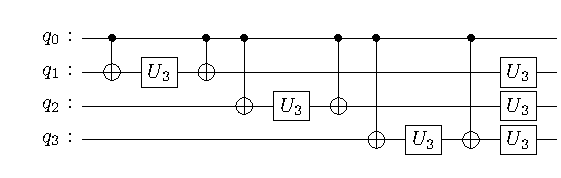
\includegraphics[width=0.55\textwidth]{figures/supplementary/rigid_block_one.pdf} \\
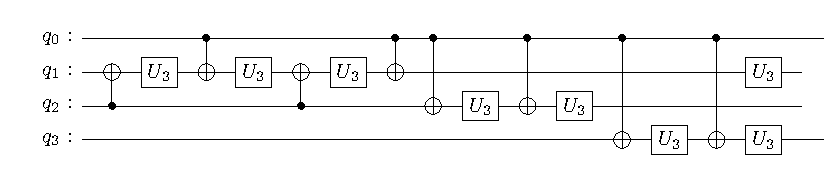
\includegraphics[width=0.8\textwidth]{figures/supplementary/rigid_block_two.pdf}
\caption{Two examples of ``rigid" circuit blocks from the QFT Adder circuit and QPE circuit.}
\label{fig:rigid_blocks}
\end{figure}

Figure \ref{fig:rigid_blocks} illustrates two examples of these rigid structures. The first block is from the QFT Adder circuit while the second block is from a QPE circuit. The first circuit contains 3 consecutive controlled rotations with the same control qubit (q0), while the second circuit contains a multi-controlled rotation and two controlled rotations. Consecutive rotations with a only a few control qubits prove difficult to reduce in the NISQ setting, since the removal of any single CNOT adds significant error to the underlying unitary. On top of that, since the control qubit is being constantly reused, it is hard to find approximate ``shortcuts" by leveraging CNOTs on surrounding qubits.

For the demonstration of our workflow shown in this work, we use a block size of $4$, while the standard BQSKit compile width is $3$. We found that by increasing the block size, both the reduction quality and probability of finding a convex hull improved, as the partitions were more likely to have many control and target qubits and be less rigid. We predict that increasing the block size to larger and larger sizes would continue to improve our results, albeit at the cost of compilation time.




\section{Statistics of ensemble error reduction}
\label{sec:error_scaling}

The benefits of using an ensemble channel are guaranteed only if the ReWEE condition is satisfied, \ie the weighted ensemble error is quadratically reduced, 
\begin{align}
    \normf{\sum_{i=1}^{M^\k} p^\k_i U^\k_i - V^\k} \leq O(\epsilon^2), 
\label{eq:wee_cond}
\end{align}
when each compilation, $U^\k_i$, is performed to error $\epsilon$.  
In practice, it is challenging to construct an ensemble of approximate circuits that both:  
\begin{enumerate}
    \item Uses fewer resource-intensive gates (e.g., CNOT or $T$ gates) on average than the original circuit, and  
    \item Satisfies Eq. \eqref{eq:wee_cond}.  
\end{enumerate}  
While explicit algorithms exist for guaranteeing Eq. \eqref{eq:wee_cond} \cite{PhysRevA.95.042306}, they are difficult to scale to multi-qubit circuits and do not provide resource efficiency guarantees.

In the main text we have shown that both criteria can be met for several of the benchmarks we studied.   
Here, we present statistics that explain how this is achieved through quadratic reduction in the weighted ensemble error and selective filtering of circuit blocks.



\begin{figure*}[t]
    \centering
    \begin{subfigure}{0.7\textwidth}
        \centering
        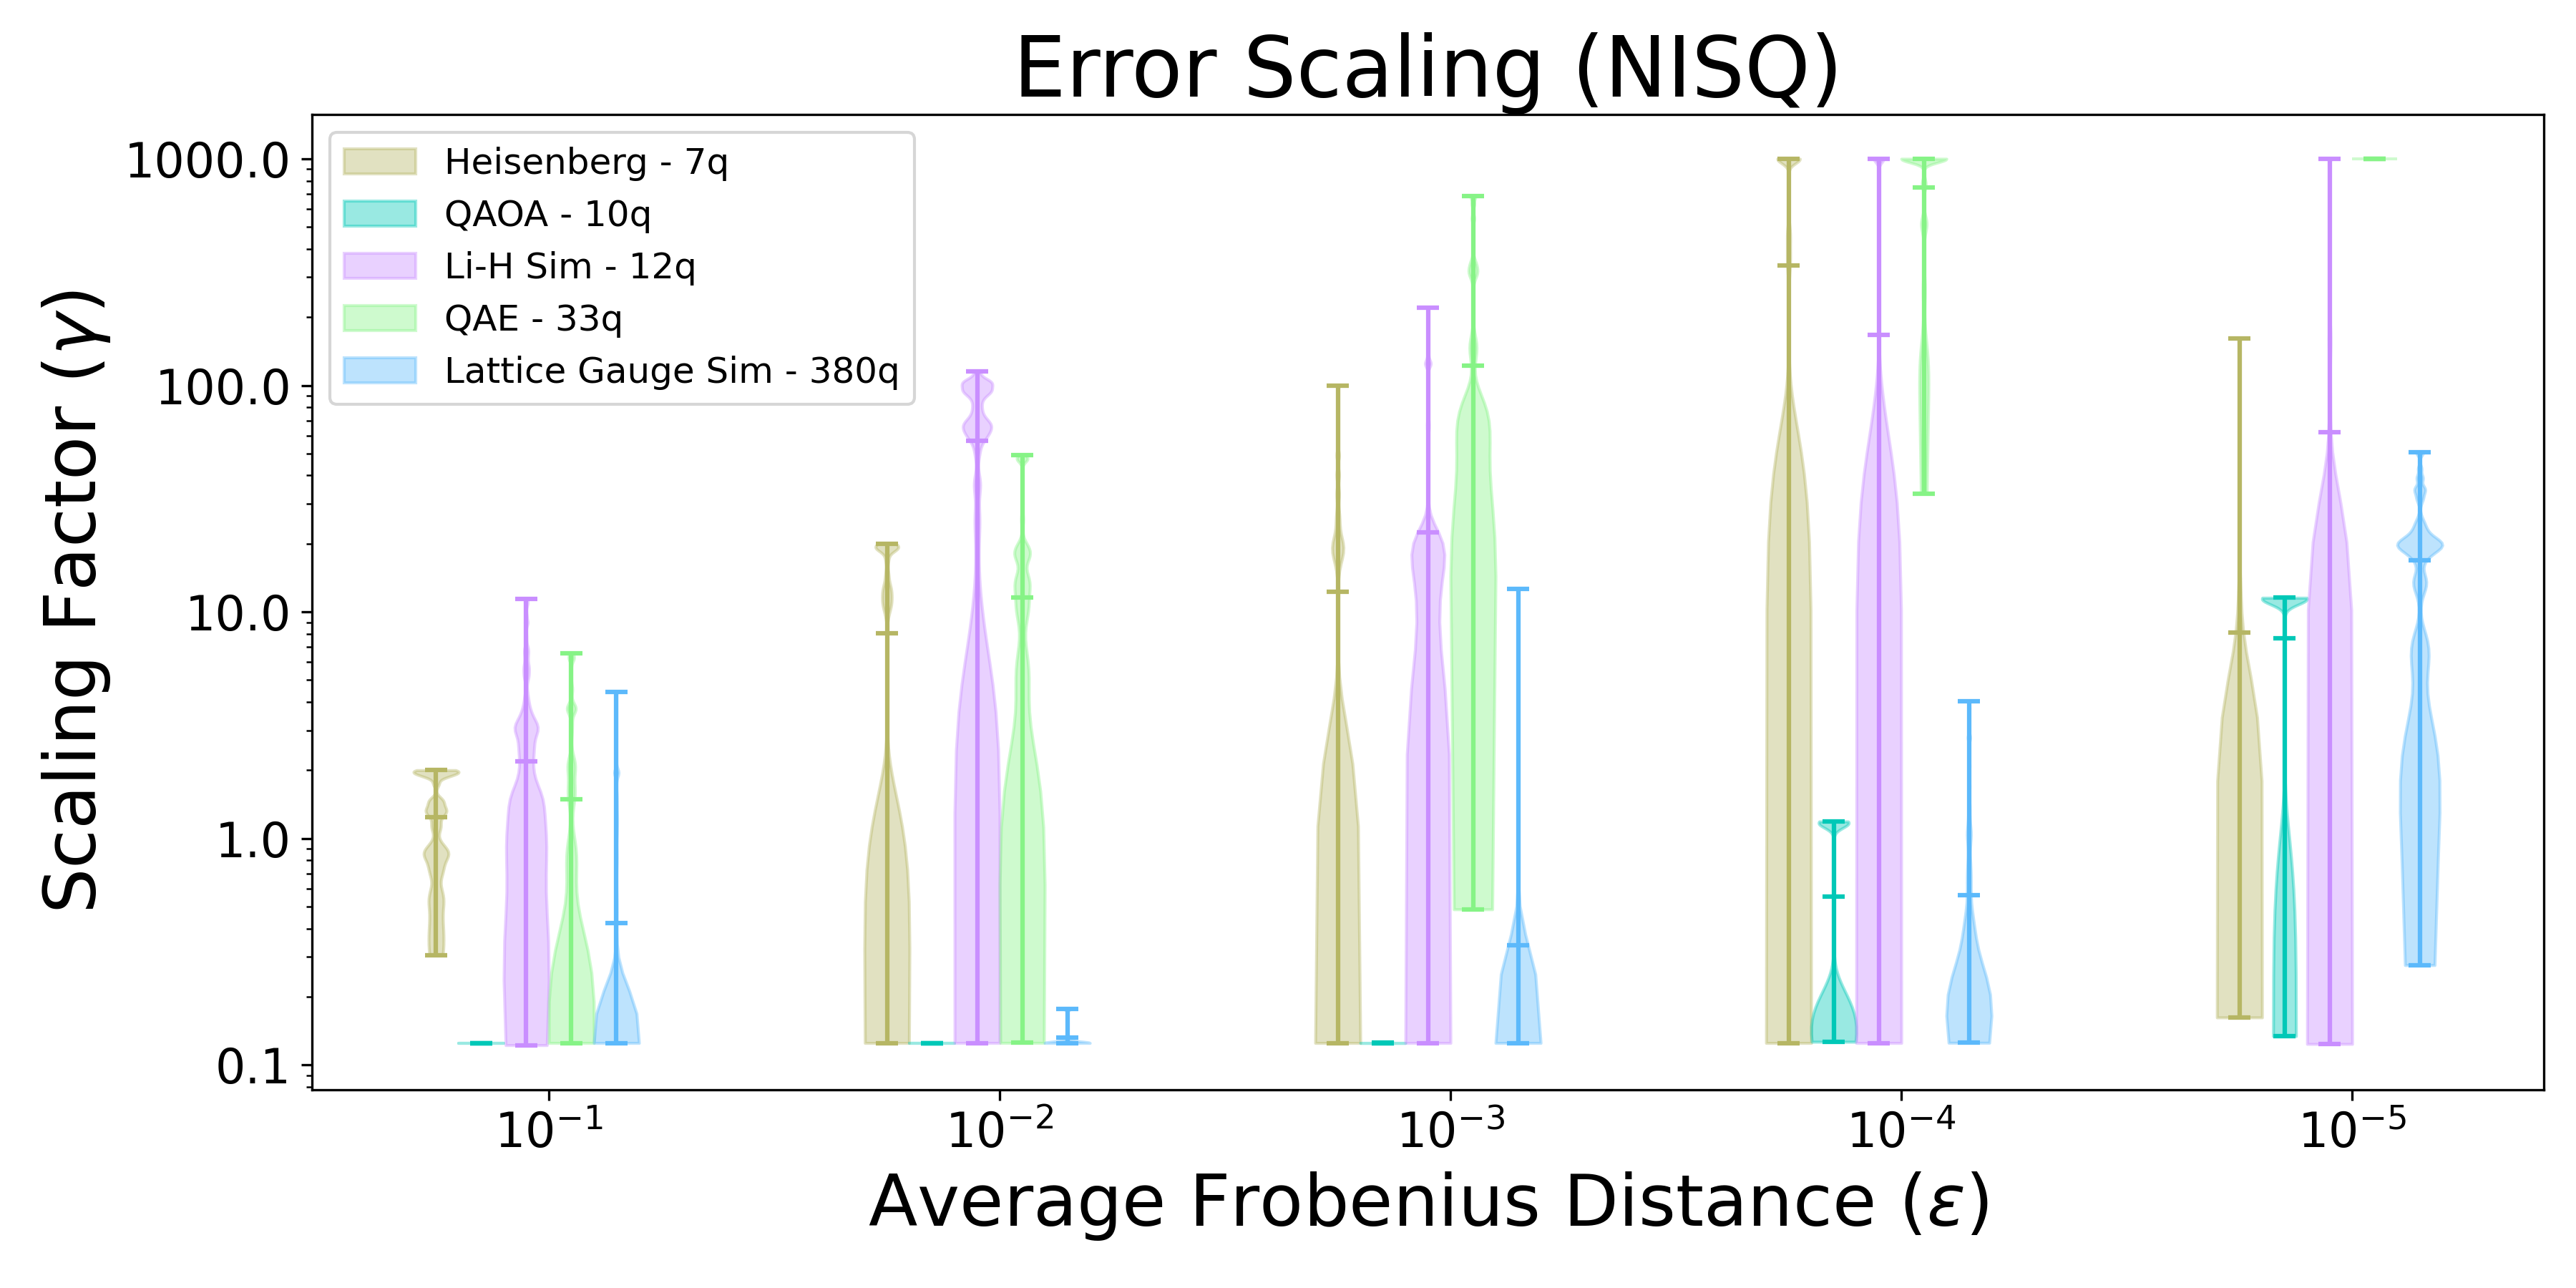
\includegraphics[width=\linewidth]{figures/supplementary/Error_scaling_final_nisq_20.png}
    \end{subfigure} \\
    \begin{subfigure}{0.7\textwidth}
        \centering
        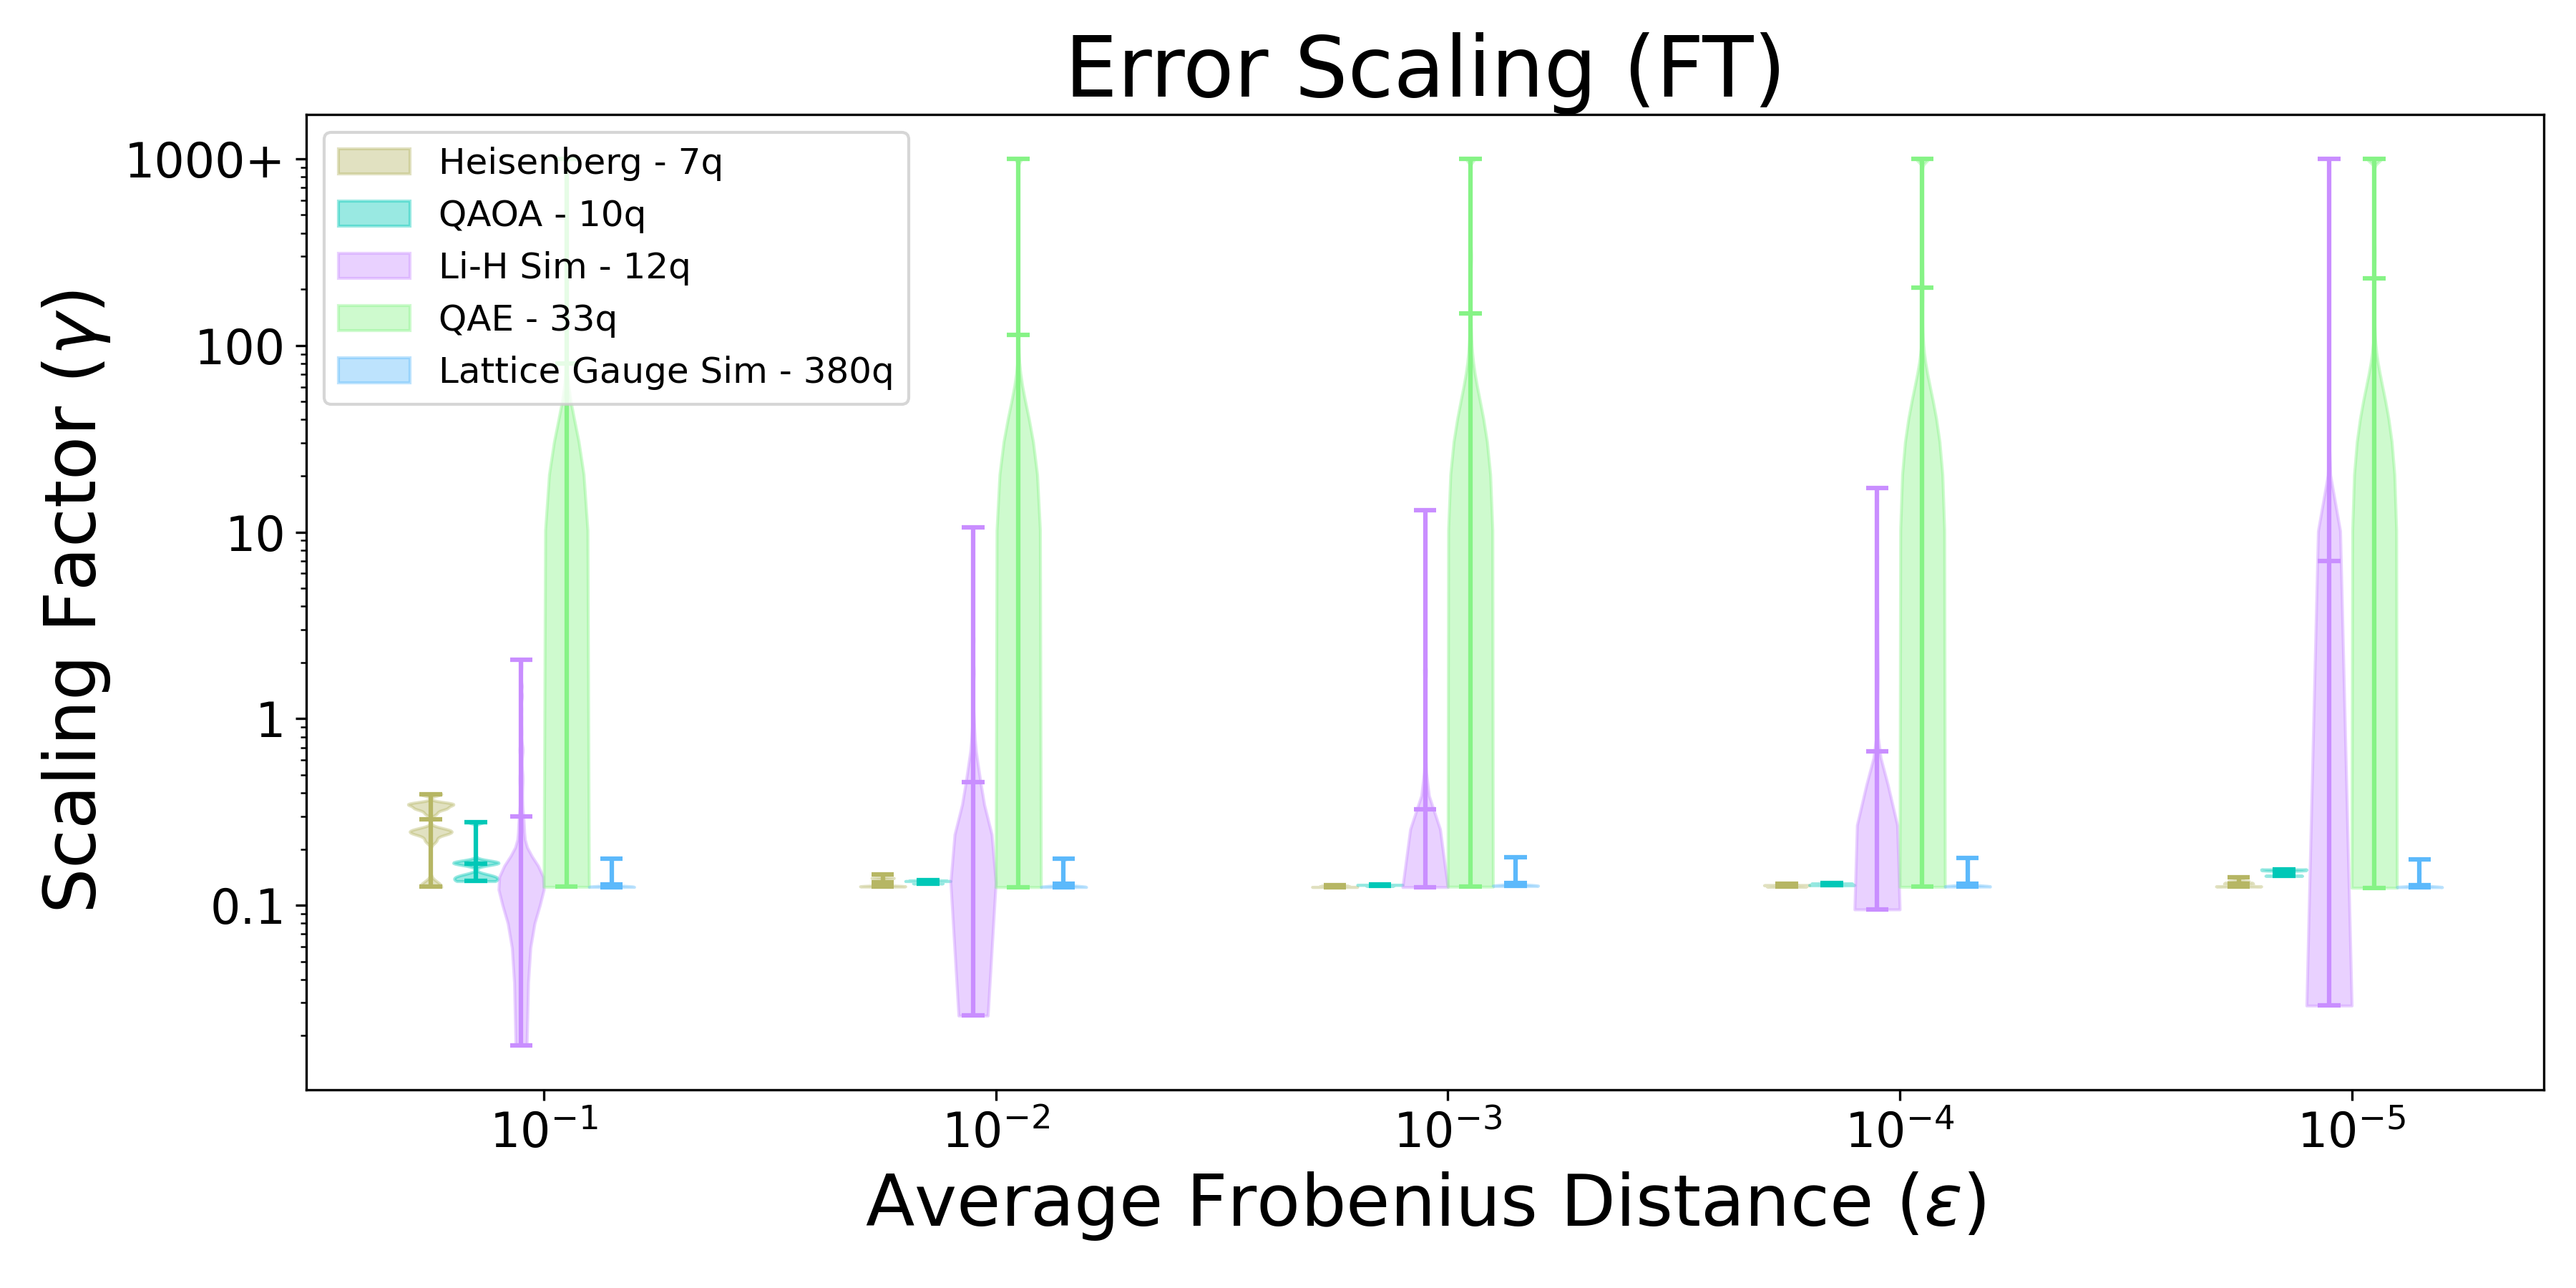
\includegraphics[width=\linewidth]{figures/supplementary/Error_scaling_final_cliff_20.png}
    \end{subfigure}
    \caption{Quadratic scaling factor $\gamma$ as a function of $\epsilon$, for some of the benchmarks.  
    Top: NISQ workflow (minimizing CNOT count).  
    Bottom: FT workflow (minimizing $T$-count).}
    \label{fig:error_scaling}
\end{figure*}


\begin{figure*}[t]
    \centering
    \begin{subfigure}{0.7\textwidth}
        \centering
        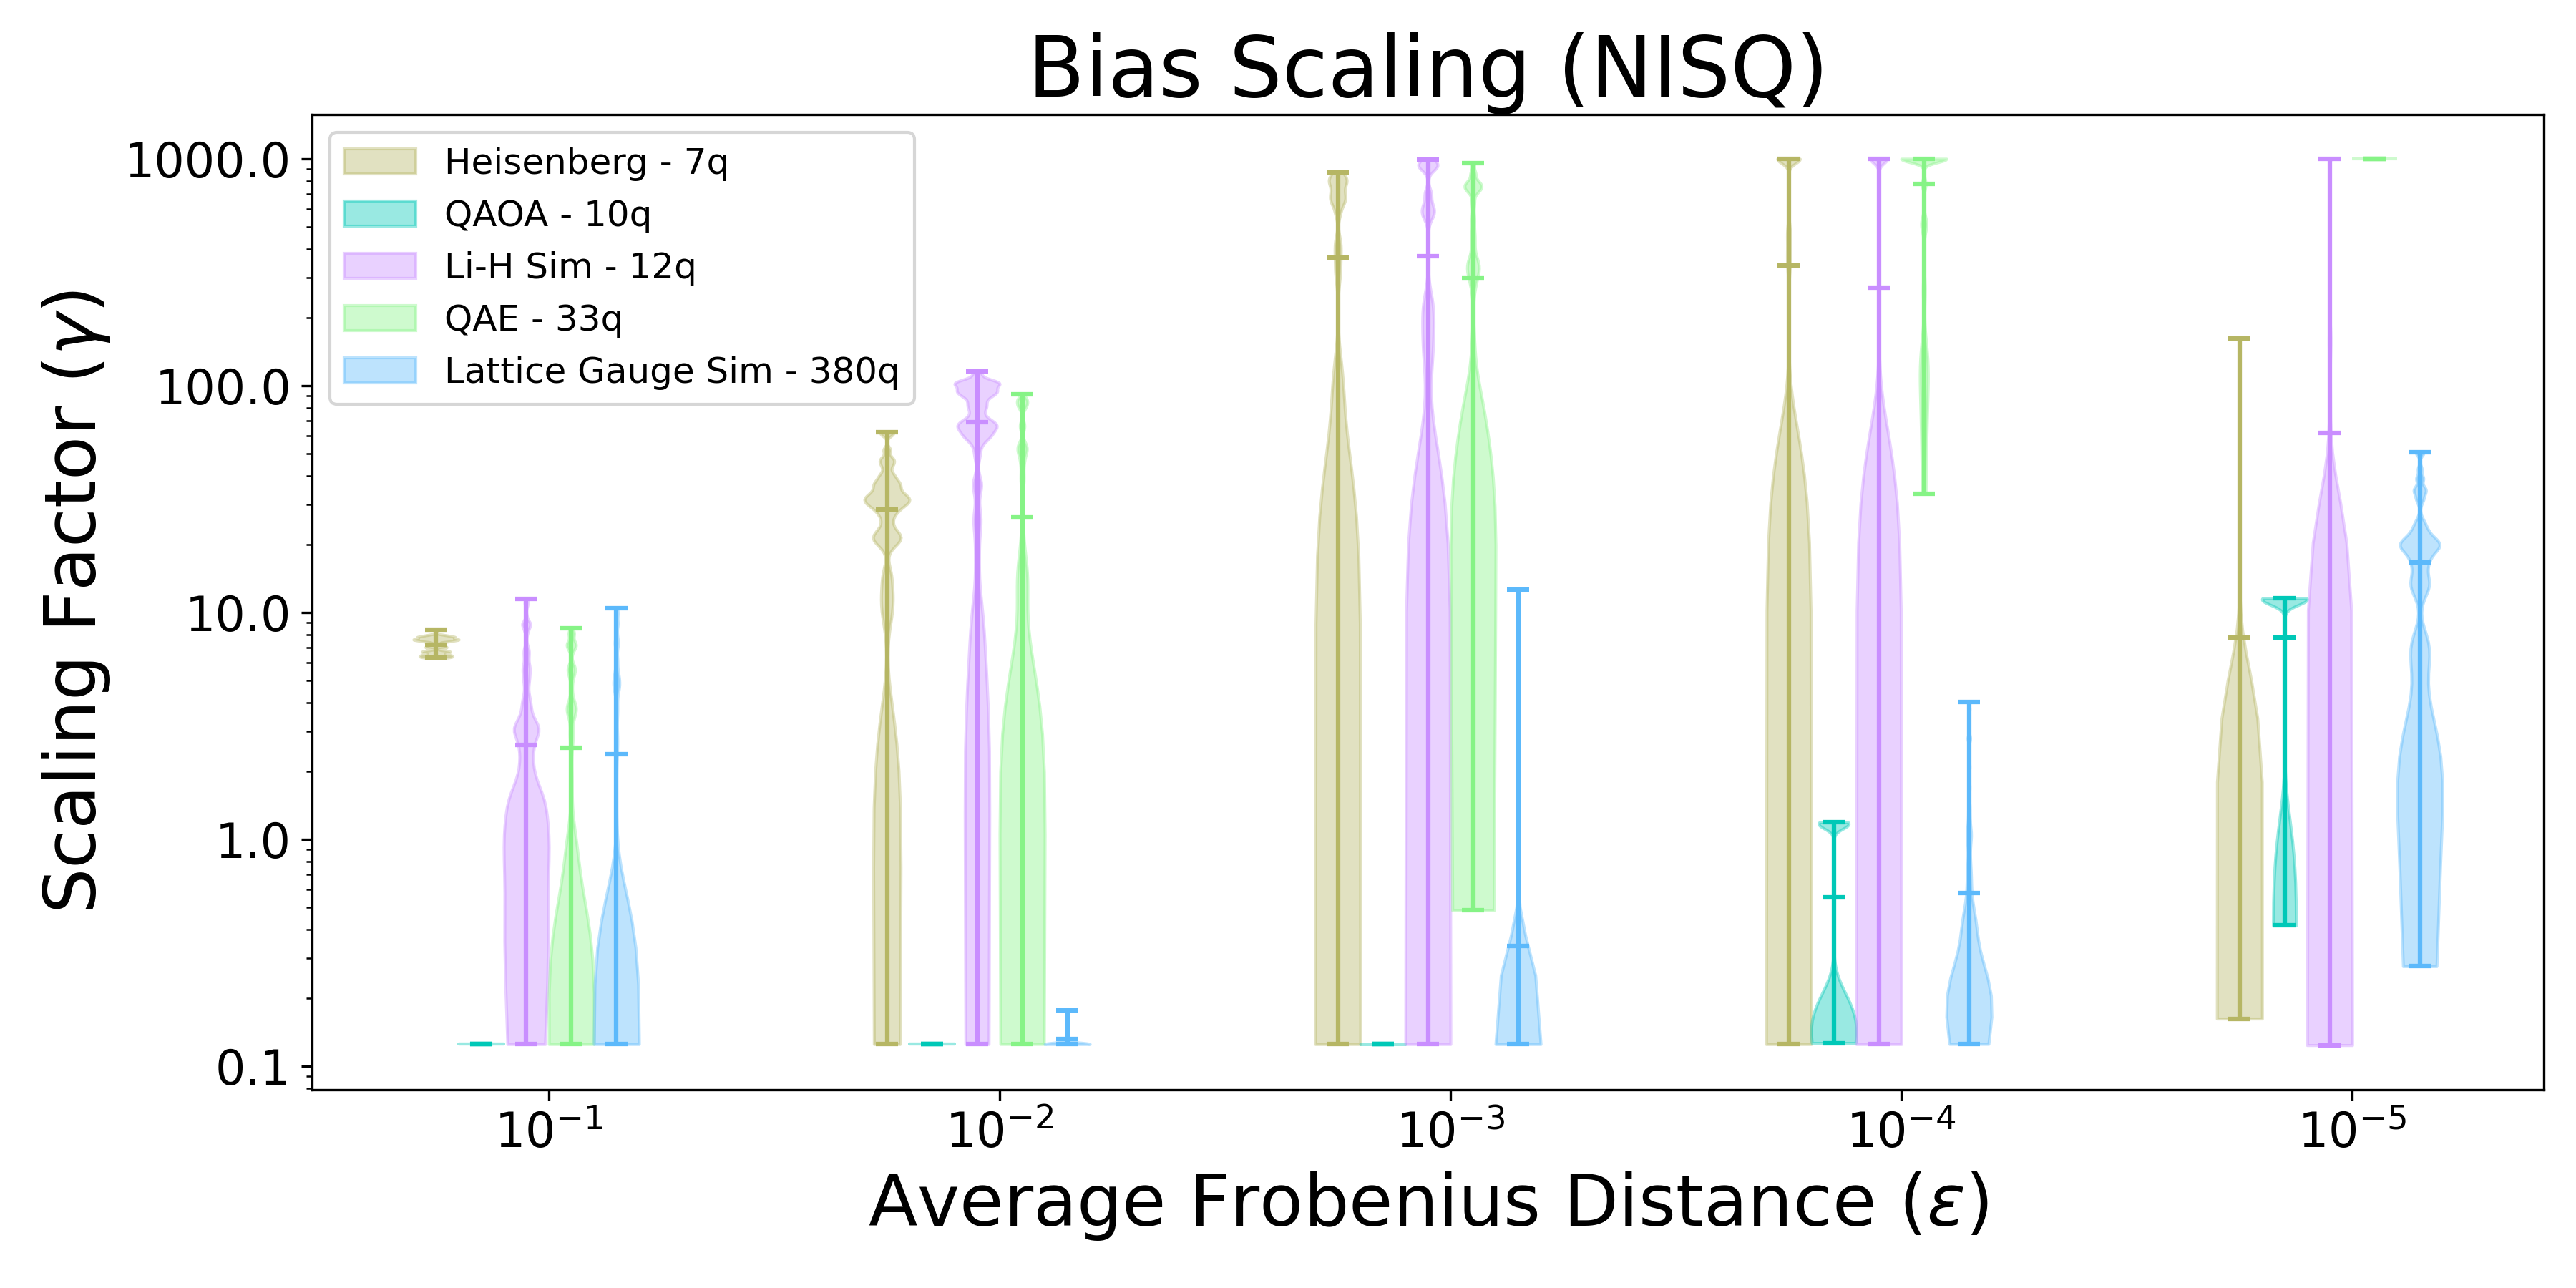
\includegraphics[width=\linewidth]{figures/supplementary/Bias_scaling_final_nisq_20.png}
    \end{subfigure} \\
    \begin{subfigure}{0.7\textwidth}
        \centering
        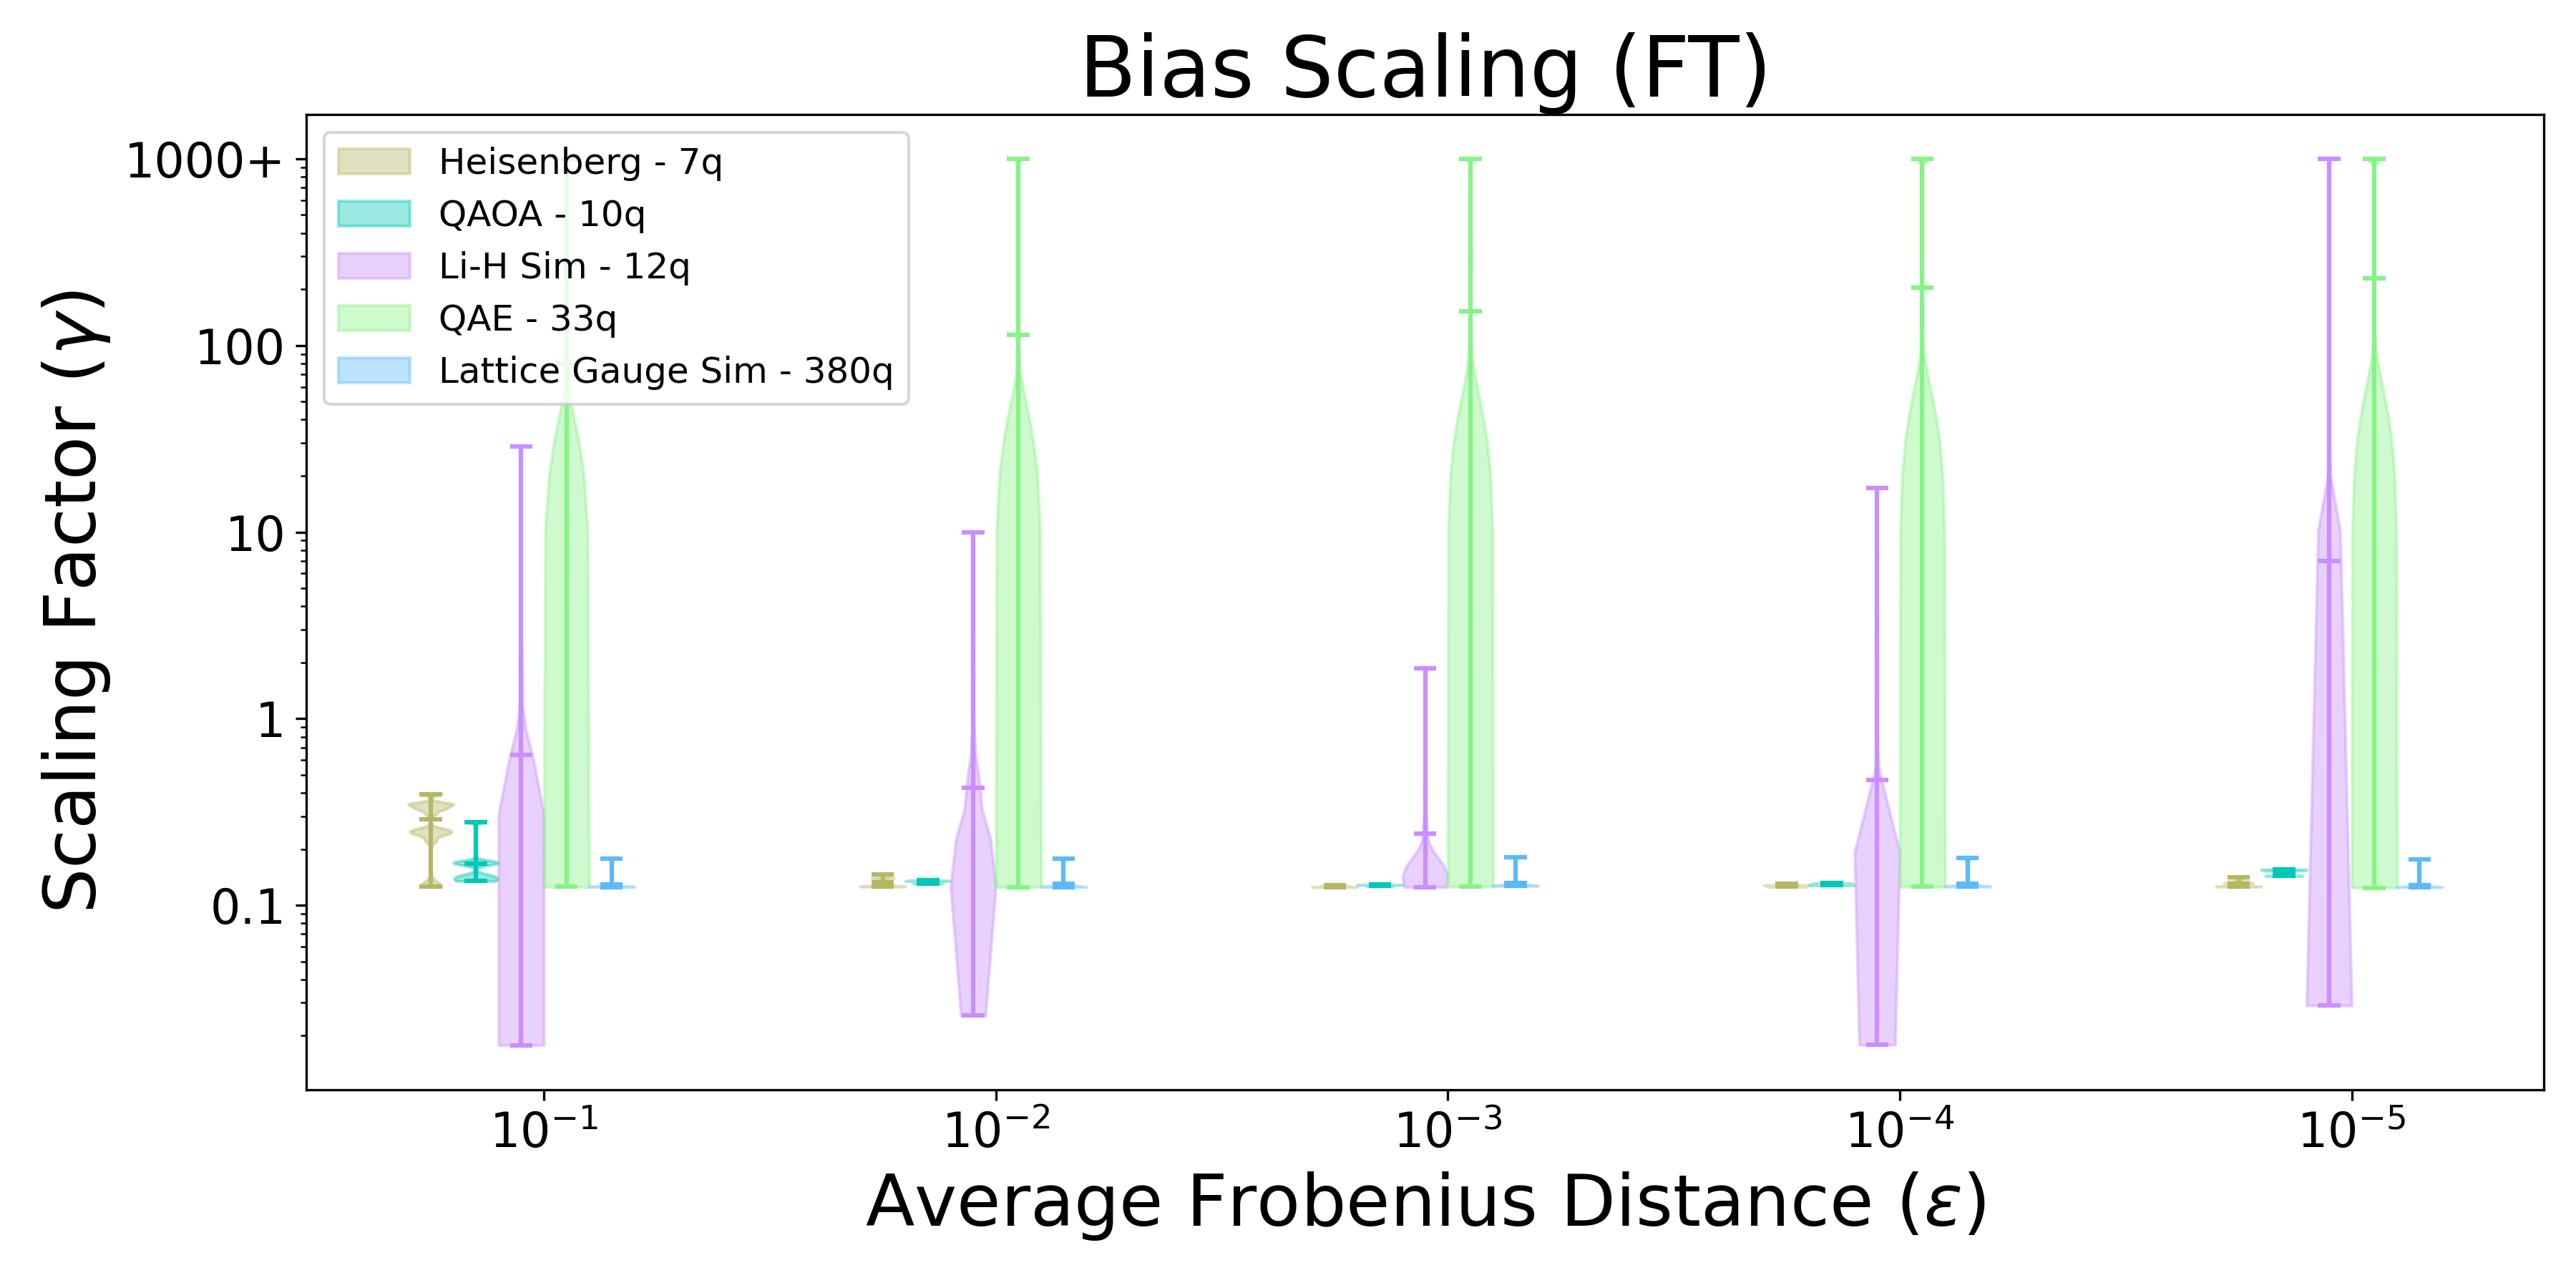
\includegraphics[width=\linewidth]{figures/supplementary/Bias_scaling_final_cliff_20.png}
    \end{subfigure}
    \caption{Quadratic scaling factor for the bias $\gamma_B$ as a function of $\epsilon$, for some of the benchmarks.  
    Top: NISQ workflow (minimizing CNOT count).  
    Bottom: FT workflow (minimizing $T$-count).}
    \label{fig:bias_scaling}
\end{figure*}

Figure \ref{fig:error_scaling} shows violin plots of the \emph{quadratic scaling factor} (QCF),  
\[
\gamma \equiv \frac{\normf{\sum_{i=1}^{M^\k} p^\k_i U^\k_i - V^\k}}{\epsilon^2},
\]  
for all blocks across many of our benchmarks.  
We expect $\gamma = O(1)$ when quadratic reduction of error is achieved.  
The plots indicate that, for most $\epsilon$ values, a significant subset of blocks in both NISQ and FT workflows achieve $O(\epsilon^2)$ scaling. In particular, almost all of the blocks in the FT workflow achieve $O(\epsilon^2)$ scaling. This is because we include a secondary compilation workflow, which trades off numerical synthesis resource reduction for improved scaling.

Our workflow does not require all blocks to satisfy Eq. \eqref{eq:wee_cond}. Blocks that fail to meet the condition are left unmodified, preserving the original circuit for those segments.  
This selective replacement explains why some benchmarks exhibit no gate count reduction (Tables 1 and 2 in the main text, particularly in the NISQ setting at small $\epsilon$). 

We also derived a sufficient condition for satisfying the ReWEE condition in terms of the bias of the compiler output,
\begin{align}
    \normf{\E{U} - V} < O(\epsilon^2).
\end{align}
We can define a quadratic scaling factor for the bias also, $\gamma_B \equiv \normf{\E{U}-V}/\epsilon^2$, and this quantity is displayed in Figure \ref{fig:bias_scaling} for all blocks of many of our benchmarks.


\section{Theoretical proofs}
In this section we provide proofs of Lemma 2 and Lemma 3 in the Methods section of the main text. Before restating the Lemmas and providing proofs, we recall several definitions from the main text.

$V$ is a target unitary on $n$ qubits, and $U_i$ are a set of approximate compilations of $V$ provided by a compiler. The compilation workflow can have probabilistic elements, and therefore we think of $U_i$ as independent, identically distributed (\emph{i.i.d.}) samples from some distribution of approximate compilations. The statistical properties we will demand of the compilation workflow are:
\begin{enumerate}
\item The compilations should all be close to the ideal, in the sense,
    \begin{align}
	\normf{U_i-V} \leq \epsilon, \quad \forall i		
		\label{eq:ass1}
	\end{align}
	\item The compilations have bounded variance, in the sense, $\E{U_i} \equiv \E{U}$ is independent of $i$, and
	\begin{align}
		\E{\normf{U_i - \E{U}}^2} \leq \epsilon', \quad \forall i
		\label{eq:ass2}
	\end{align}
\end{enumerate}
The expectations in these expressions and in the rest of this note are over the distribution of compilations generated by the compiler that satisfy Condition 1, \ie
$ \E{f(U)} = \int {\rm d}\mu_V(U) f(U), $
where ${\rm d}\mu_V(U)$ is the measure over $SU(2^n)$ defined by the compiler output that satisfies Condition 1 when the target is $V$ (the expectation symbol $\E{}$ should have a subscript $V$ but we omit this for ease). In addition,
\begin{enumerate}
    \item Define the channels $\mathcal{V}[\rho] = V \rho V\dg$, $\mathcal{U}_i[\rho] = U_i \rho U_i\dg$, and $\mathcal{U}[\rho] = \sum_i p_i U_i \rho U_i\dg$, for some probabilities $\{p_i\}$.
    \item $J_{\mathcal{E}} \equiv \sum_{i,j=1}^d \mathcal{E}(\ket{i}\bra{j})\otimes \ket{i}\bra{j}$ is the Choi matrix representation of the channel $\mathcal{E}$, which we assume to be acting acting on $d\times d$ density matrices and outputting density matrices of the same size.
\end{enumerate}

\noindent \emph{\bf Lemma 2:} \emph{Let $V$ and $U_i$ be defined as above. Given probabilities $\{p_i\}_{i=1}^M$, ($\sum_{i=1}^M p_i=1$), a sufficient condition for achieving $\E{\normf{\sum_{i=1}^M p_i U_i - V}} \leq O(\epsilon^2)$ is the \emph{reduced bias condition}: $\normf{\E{U}-V} \leq O(\epsilon^2)$.}

\noindent \textit{Proof:} First, note that $\E{\normf{\sum_{i=1}^M p_i U_i - V}} \leq O(\epsilon^2)$ follows directly from $\E{\normf{\sum_{i=1}^M p_i U_i - V}^2} \leq O(\epsilon^4)$ through an application of Jensen's inequality, and so we prove the latter statement.
\begin{align}
    \E{\normf{\sum_{i=1}^M p_i U_i - V}^2} & \leq \E{\normf{\frac{1}{M}\sum_{i=1}^M U_i - V}^2} 
	   = \normf{\overline{bias}}^2 + \frac{1}{M}\overline{var} + \left(1-\frac{1}{M}\right)\overline{covar}, 
       \label{eq:b-v-c} 
\end{align}
where,
\begin{align}
	\overline{bias} &= (\E{U} - V) \label{eq:bias} \\
	\overline{var} &= \frac{1}{M}\sum_{i=1}^{M} \E{\normf{U_i - \E{U}}^2} \label{eq:var} \\
	\overline{covar} &= \frac{1}{M(M-1)}\sum_{i=1}^M \sum_{j \neq i}^M \mathbb{E} \left\{ \tr[(U_i-\E{U})\dg \cdot (U_j - \E{U})] \right\} 
    \label{eq:covar}
\end{align}
The first inequality follows from the fact that the weights $p_i$ are optimized to reduce the ensemble error. The equality on the second line follows from using the definition of the Frobenius norm to decompose the quantity of interest in a \emph{bias-variance-covariance} decomposition, a well-known decomposition of generalization error of ensembles of estimators in machine learning \cite{Ueda_1996, Brown_20005}. Here, $\overline{bias}$ is the bias of the (uniform) ensemble, $\overline{var}$ is the (sample) average of the variance of the members of the ensemble, and $\overline{covar}$ is the covariance of the ensemble members. Since the ensemble members are sampled \emph{i.i.d.} from the compiler output distribution, the covariance term is zero. In addition, using the fact that the samples have bounded variance, Eq. \eqref{eq:ass2}, we get
$\E{\normf{\sum_{i=1}^M p_i U_i - V}^2} \leq \normf{\E{U}-V}^2 + \frac{\epsilon'}{M}$.
This quantity can be bounded as $O(\epsilon^4)$ by satisfying the reduced bias condition and choosing $M \geq \epsilon'/\epsilon^4$. \QED
\\

\noindent \emph{\bf Lemma 3:} \emph{Let $V$ and $U_i$ be defined as above, and let these unitaries act on a register of $n$ qubits; \ie ${\rm dim}~ V = {\rm dim}~ U_i = 2^n \equiv d$. Define $\mathcal{V}[\rho] = V \rho V^{\dagger}$ as a target channel, and $\mathcal{U}[\rho] = \sum_{i=1}^M p_i U_i \rho U_i\dg$ as an optimized ensemble channel, such that $d_\diamond(\mathcal{V}, \mathcal{U})\leq O(\epsilon^2)$. Further, let $\hat{\mathcal{U}}[\rho] = \frac{1}{T}\sum_{i=1}^T U_{\sigma(i)} \rho U_{\sigma(i)}\dg$ be the empirical channel defined by sampling and averaging over $U_i$ according to the distribution $\{p_i\}$ -- \ie $\sigma(i) \in \{1,...,M\}$. For $\epsilon, \delta \in (0,1)$, $\pr\left\{ d_\diamond(\mathcal{V}, \hat{\mathcal{U}}_T) \leq O(\epsilon^2) \right\} > 1-\delta$, given
\begin{align}
    T \geq \frac{2v + \frac{2}{3}R \left(\epsilon^2/(2d^2)\right) }{\left(\epsilon^2/(2d^2)\right)^2}\log \frac{2d^2}{\delta}
    \label{eq:T_bound}
\end{align}
Here, $v \equiv \normo{\sum_{i=1}^M p_i (J_i - J_{\mathcal{U}})^2}, R \equiv \max_i \normo{J_i - J_{\mathcal{U}}}$, and $J_i (and J_{\mathcal{U}}$) are the $d^2$-dimensional Choi matrices associated to the channel $\mathcal{U}_i[\rho] = U_i \rho U_i^{\dagger}$ (and $\mathcal{U}$).}

\noindent \textit{Proof:} We begin by an application of the triangle inequality:
\begin{align}
    d_\diamond(\mathcal{V}, \hat{\mathcal{U}}) &\leq  d_\diamond(\mathcal{V}, \mathcal{U}) +  d_\diamond(\mathcal{U}, \hat{\mathcal{U}}) \nn \\  
    & = O(\epsilon^2) + d_\diamond(\mathcal{U}, \hat{\mathcal{U}}),
    \label{eq:lemma3_1}
\end{align}
and hence we are left with the task of determining the sample size $T$ necessary to satisfy $d_\diamond(\mathcal{U}, \hat{\mathcal{U}}) \leq \epsilon^2$. Therefore, 
\begin{align}
    d_\diamond(\mathcal{U}, \hat{\mathcal{U}}) &\equiv \normd{\mathcal{U}- \hat{\mathcal{U}}} \nn \\
    & \leq \normt{J_\mathcal{U} - J_{\hat{\mathcal{U}}}} \nn \\
    & \leq 2d^2 \normo{J_\mathcal{U} - J_{\hat{\mathcal{U}}}},
\end{align}
where the first inequality follows from an identity established by Watrous \cite[Exercise 3.6]{watrous_2018}, the second is the application of a standard norm inequality ($\normt{A}\leq {\rm rank}(A)\normo{A}$), and an overestimate of the relevant rank: ${\rm rank}(J_\mathcal{U} - J_{\hat{\mathcal{U}}}) \leq {\rm rank}(J_\mathcal{U} ) + {\rm rank}(J_{\hat{\mathcal{U}}}) \leq 2d^2$. In the above, the Choi matrices are explicitly, $J_\mathcal{U} = \sum_{i=1}^M p_i J_i$ and $J_{\hat{\mathcal{U}}} = \frac{1}{T} \sum_{i=1}^T J_i$, with $J_i \equiv J_{\mathcal{U}_i}$. 

Now that the error is expressed in terms of an operator norm, we can apply standard Bernstein matrix concentration inequality \cite{tropp_2015} to get, 
\begin{align}
    \pr\left\{ d_\diamond(\mathcal{U}, \hat{\mathcal{U}}) \geq \epsilon^2 \right\} \leq \pr\left\{ \normo{J_\mathcal{U} - J_{\hat{\mathcal{U}}}} \geq \frac{\epsilon^2}{2d^2} \right\} \leq 2d^2 \exp\left(-\frac{T(\frac{\epsilon^2}{2d^2})^2}{2v + \frac{2}{3}R \frac{\epsilon^2}{2d^2}}\right),
\end{align} 
where $v$ and $R$ are the variance and maximum deviation as defined in the Lemma statement. In order for the right-hand side to be at most $\delta$, the sample size given in Eq. \eqref{eq:T_bound} is sufficient. Finally, combining this with the statement in Eq. \eqref{eq:lemma3_1} yields the Lemma statement. 
\QED

\subsection{Statistics of factors entering sample complexity}
While the formal sample complexity bound in Lemma 3 scales with $\epsilon$ as $O(1/\epsilon^4)$, in the main text we claimed that in practice, $v=O(\epsilon^2)$, and therefore, the number of samples needed is $O(1/\epsilon^2)$. Figure 5 in the main text provided evidence for this gentler scaling for one of the benchmarks in our study. While Lemma 3 is stated in terms of diamond distance between the empirical channel and the ensemble channel, this error is infeasible to evaluate numerically because of the difficulty of calculating the diamond distance for channels acting on many qubits. Therefore, in Figure 5 of the main text, we showed the trace distance error in the output, $\normt{\rho_{T} - \rho_i}$,
where $\rho = \sum_{i=1}^M p_i U_i \rho_{0} U_i\dg$ is the output of the ensemble channel for random input state $\rho_{0}$, and $\rho_{T} = \frac{1}{T}\sum_{i=1}^T U_i \rho_{0} U_i\dg$ is the output of the empirical channel for the same input (the $U_i$ in the empirical channel are sampled according to the distribution $\{p_i\}$ set by the ensemble channel). 

The equivalent sample complexity bound for this error metric is $\pr\{\normt{\rho_{T} - \rho} \geq \epsilon^2\} \leq 1-\delta$, if
\begin{align}
    T \geq \frac{2v + \frac{2}{3}R \left(\epsilon^2/(2d)\right) }{\left(\epsilon^2/(2d)\right)^2}\log \frac{2d}{\delta},
    \label{eq:T_bound_state} 
\end{align}
where $v \equiv \normo{\sum_{i=1}^M p_i (\rho_i - \rho)^2}, R \equiv \max_i \normo{\rho_i - \rho}$, and $\rho_i = U_i\rho_0 U_i\dg$. Calculating the values $v$ and $R$ is difficult for most of the benchmarks we studied, even in this case, because $M$ can be very large for full circuits, and thus computing the ideal ensemble output $\rho$ is numerically intensive. Instead, we compute these variance and maximum deviation values, $v$ and $R$, for all blocks in two of our benchmark circuit ensembles. As shown in Fig. \ref{fig:vR}, $v \ll \epsilon^2$ in practice, which explains the gentler scaling of $T$ required to approximate the ensemble channel with the empirical channel.

\begin{figure*}[ht]
    \centering
        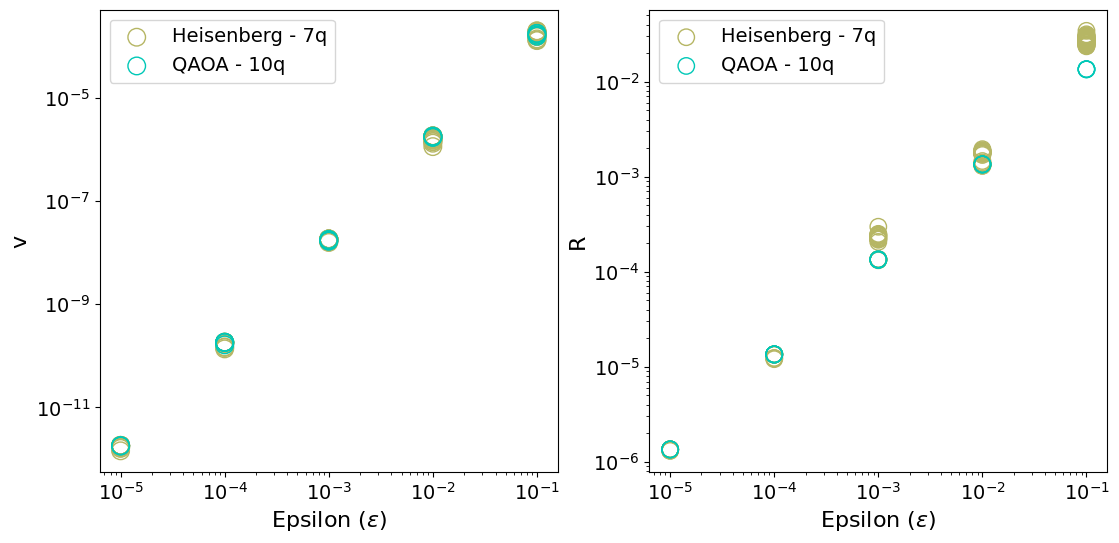
\includegraphics[width=0.7\linewidth]{figures/supplementary/v_R_all_circs_1_final.png}
    \caption{Values of variance and maximum deviation factors, $v$ and $R$, entering the sample complexity bound Eq. \eqref{eq:T_bound_state} for each block of two benchmark circuits.}
    \label{fig:vR}
\end{figure*}

\newpage

\documentclass[fleqn,10pt]{wlscirep}
\usepackage[utf8]{inputenc}
\usepackage[T1]{fontenc}
\usepackage{wrapfig}
\usepackage{subcaption}
\usepackage{multirow}
\usepackage{multicol}
\usepackage{tikz}
\usepackage{graphicx}
\usepackage{standalone}

\newcommand{\eg}{\emph{e.g.,~}}
\newcommand{\ie}{\emph{i.e.,~}}
\newcommand{\bx}{\mathbf{x}}
\newcommand{\by}{\mathbf{y}}
\newcommand{\bp}{\mathbf{p}}
\newcommand{\hx}{\hat{x}}
\newcommand{\hp}{\hat{p}}
\newcommand{\ket}[1]{\vert#1\rangle}
\newcommand{\bra}[1]{\langle #1\vert}
\newcommand{\expect}[1]{\langle #1\rangle}
\newcommand{\dg}{^\dagger}
\newcommand{\nn}{\nonumber}
\newcommand{\pr}{{\rm Pr}}

\newcommand{\normf}[1]{\left\lVert #1 \right\rVert_F}
\newcommand{\normo}[1]{\left\lVert #1 \right\rVert}
\newcommand{\normt}[1]{\left\lVert #1 \right\rVert_1}
\newcommand{\normd}[1]{\left\lVert #1 \right\rVert_\diamond}
\newcommand{\E}[1]{\mathbb{E}\left\{ #1 \right\}}

\newcommand{\tr}{{\rm tr}}
\renewcommand{\k}{{(k)}}
\newcommand{\p}{{\bf\sf p}}
\newcommand{\braket}[2]{\langle #1 \vert #2 \rangle}

\newcommand*{\QED}{\null\nobreak\hfill\ensuremath{\blacksquare}}%

\makeatletter
\renewcommand{\@maketitle}{%
{%
\thispagestyle{empty}%
\vskip-36pt%
{\raggedright\sffamily\bfseries\fontsize{20}{25}\selectfont \@title\par}%
\vskip10pt
{\raggedright\sffamily\fontsize{12}{16}\selectfont  \@author\par}
\vskip25pt%
}%
}%
\makeatother

\newcommand{\red}[1]{{\color{red}#1}} 
\newcommand{\needcite}{{\color{red}[XX]~}}
\long\def\comment#1{}
\long\def\note#1{{\em #1 }}
\def\parah#1{\vspace*{0.0in} \noindent{\bf #1:}}

\title{Supplementary Information for: Application Scale Quantum Circuit Compilation with Controlled Error}

\author[1,2,*]{Justin Kalloor}
\author[3]{Lucas Kovalsky}
\author[1,2]{Mathias Weiden}
\author[2]{John Kubiatowicz}
\author[1]{Ed Younis}
\author[1]{Costin Iancu}
\author[3,+]{Mohan Sarovar}
\affil[1]{Computational Research Division, Lawrence Berkeley National Laboratory, Berkeley, CA, 94702, USA}
\affil[2]{Department of Electrical Engineering and Computer Science, University of California, Berkeley, CA, 94702, USA}
\affil[3]{Quantum Algorithms and Applications Collaboratory, Sandia National Laboratories, Livermore, CA, 94550, USA}

\affil[*]{jkalloor3@berkeley.edu}
\affil[+]{mnsarov@sandia.gov}



\begin{document}

\flushbottom
\maketitle

\section{Description of benchmark applications and circuits}
For our benchmarks, we use a variety of quantum algorithms across different domains of interest.

\subsection*{Hamiltonian Simulation Algorithms}
\begin{enumerate}
    \item \textbf{SU(2) Lattice Gague Simulation} - We follow the construction outlined in the paper by Rahman et. al \cite{rahman_2022} to simulate the motion of an excitation on a spatial lattice.
    \item \textbf{Li-H Molecule} - We simulate the electronic energy of a Lithium Hydride molecule. The circuit was generated using the Qiskit Nature and PySCF\cite{qiskit} libraries. The fermionic operator was mapped to qubits using a Jordan Wigner mapper\cite{jordan_wigner}. When calculating the observable, we use the Hartree Fock \cite{hartree_fock} state as the initial state.
    \item \textbf{Fermi-Hubbard Model} We run the Fermi-Hubbard model on a square lattice with periodic boundary conditions. The lattice has uniform interaction energies as well as a uniform onsite potential and was mapped to a quantum circuit with a Jordan Wigner mapper. For the observable calculations, we pass in the ground state of the non-interacting model as the initial state.
    \item \textbf{Heisenberg Model} - We simulate the nearest neighbor Heisenberg model with the Hamiltonian defined as:
    \[H = J \cdot \sum{X_iX_{i+1} + Y_iY_{i+1} + Z_iZ_{i+1}}\] and use the all zero state as the initial ground state.
\end{enumerate}

\subsection*{Arithmetic Sub-Modules}

\begin{enumerate}
    \item \textbf{Multiplier} - A quantum sub-circuit to multiply two registers and store into an output register\cite{qiskit}.
    \item \textbf{Adder} - A simple implementation of a Ripple-Carry Adder to add together two quantum registers \cite{qiskit}.
    \item \textbf{QFT Adder} - An implementation of the Draper QFT Adder \cite{draper}.
\end{enumerate}

\subsection*{Quantum Sub-Routines}

\begin{enumerate}
    \item \textbf{Quantum Amplitude Estimation (QAE)} - An implementation of the quantum amplitude estimation circuit on a Bernoulli Operator with a probability of 0.5 \cite{qiskit, brassard}.
    \item \textbf{Quantum Phase Estimation (QPE)} - We estimate the phase of a randomly generated circuit. In our 14 qubit example, we generate a 7-qubit random circuit, and use 7 qubits for precision.
\end{enumerate}

\subsection*{Quantum Optimization}

\begin{enumerate}
    \item Quantum Approximate Optimization Algorithm - An implementation of the optimization circuit given in QASMBench\cite{qasm_bench}.
\end{enumerate}

\section{``Rigid" Circuit Blocks}
\label{sec:rigid_blocks}
As ensemble generation time grows exponentially with the number of qubits, circuit partitioning allows us to scale our workflow to application-width circuits. We first split our circuit into blocks of width $w$, and then generate a block-level ensemble for each partition \emph{in parallel}. Importantly, we are able to accept/reject each ensemble based on the ReWEE condition, which gives us additional flexibility on which circuits benefit from our methodology. We do not need a perfect ensemble for the circuit as a whole; we can pick and choose which parts of the circuit benefit from approximation.

Despite this additional freedom provided by the partitioner, there are benchmarks that are unable to see any reduction in the NISQ compilation workflow. This happens when the input circuit is partitioned into ``rigid" blocks. Rigid blocks are circuits (along with their underlying unitaries) that either 1) Cannot be reduced (e.g no CNOTs can be removed without significant approximation error or 2) Only have a few approximate solutions, which are not diverse enough to form a convex hull around the original unitary.

\begin{figure}[htbp]
\centering
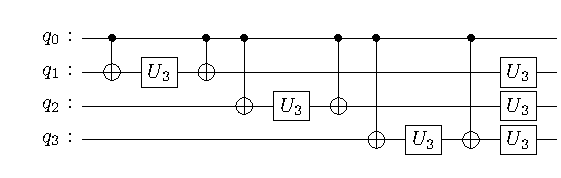
\includegraphics[width=0.55\textwidth]{figures/supplementary/rigid_block_one.pdf} \\
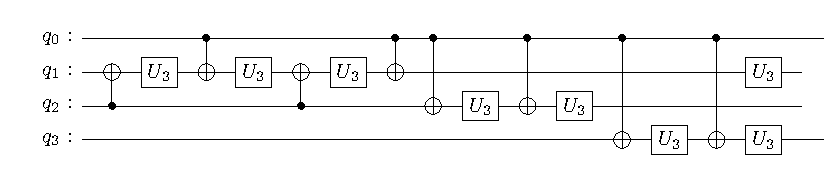
\includegraphics[width=0.8\textwidth]{figures/supplementary/rigid_block_two.pdf}
\caption{Two examples of ``rigid" circuit blocks from the QFT Adder circuit and QPE circuit.}
\label{fig:rigid_blocks}
\end{figure}

Figure \ref{fig:rigid_blocks} illustrates two examples of these rigid structures. The first block is from the QFT Adder circuit while the second block is from a QPE circuit. The first circuit contains 3 consecutive controlled rotations with the same control qubit (q0), while the second circuit contains a multi-controlled rotation and two controlled rotations. Consecutive rotations with a only a few control qubits prove difficult to reduce in the NISQ setting, since the removal of any single CNOT adds significant error to the underlying unitary. On top of that, since the control qubit is being constantly reused, it is hard to find approximate ``shortcuts" by leveraging CNOTs on surrounding qubits.

For the demonstration of our workflow shown in this work, we use a block size of $4$, while the standard BQSKit compile width is $3$. We found that by increasing the block size, both the reduction quality and probability of finding a convex hull improved, as the partitions were more likely to have many control and target qubits and be less rigid. We predict that increasing the block size to larger and larger sizes would continue to improve our results, albeit at the cost of compilation time.




\section{Statistics of ensemble error reduction}
\label{sec:error_scaling}

The benefits of using an ensemble channel are guaranteed only if the ReWEE condition is satisfied, \ie the weighted ensemble error is quadratically reduced, 
\begin{align}
    \normf{\sum_{i=1}^{M^\k} p^\k_i U^\k_i - V^\k} \leq O(\epsilon^2), 
\label{eq:wee_cond}
\end{align}
when each compilation, $U^\k_i$, is performed to error $\epsilon$.  
In practice, it is challenging to construct an ensemble of approximate circuits that both:  
\begin{enumerate}
    \item Uses fewer resource-intensive gates (e.g., CNOT or $T$ gates) on average than the original circuit, and  
    \item Satisfies Eq. \eqref{eq:wee_cond}.  
\end{enumerate}  
While explicit algorithms exist for guaranteeing Eq. \eqref{eq:wee_cond} \cite{PhysRevA.95.042306}, they are difficult to scale to multi-qubit circuits and do not provide resource efficiency guarantees.

In the main text we have shown that both criteria can be met for several of the benchmarks we studied.   
Here, we present statistics that explain how this is achieved through quadratic reduction in the weighted ensemble error and selective filtering of circuit blocks.



\begin{figure*}[t]
    \centering
    \begin{subfigure}{0.7\textwidth}
        \centering
        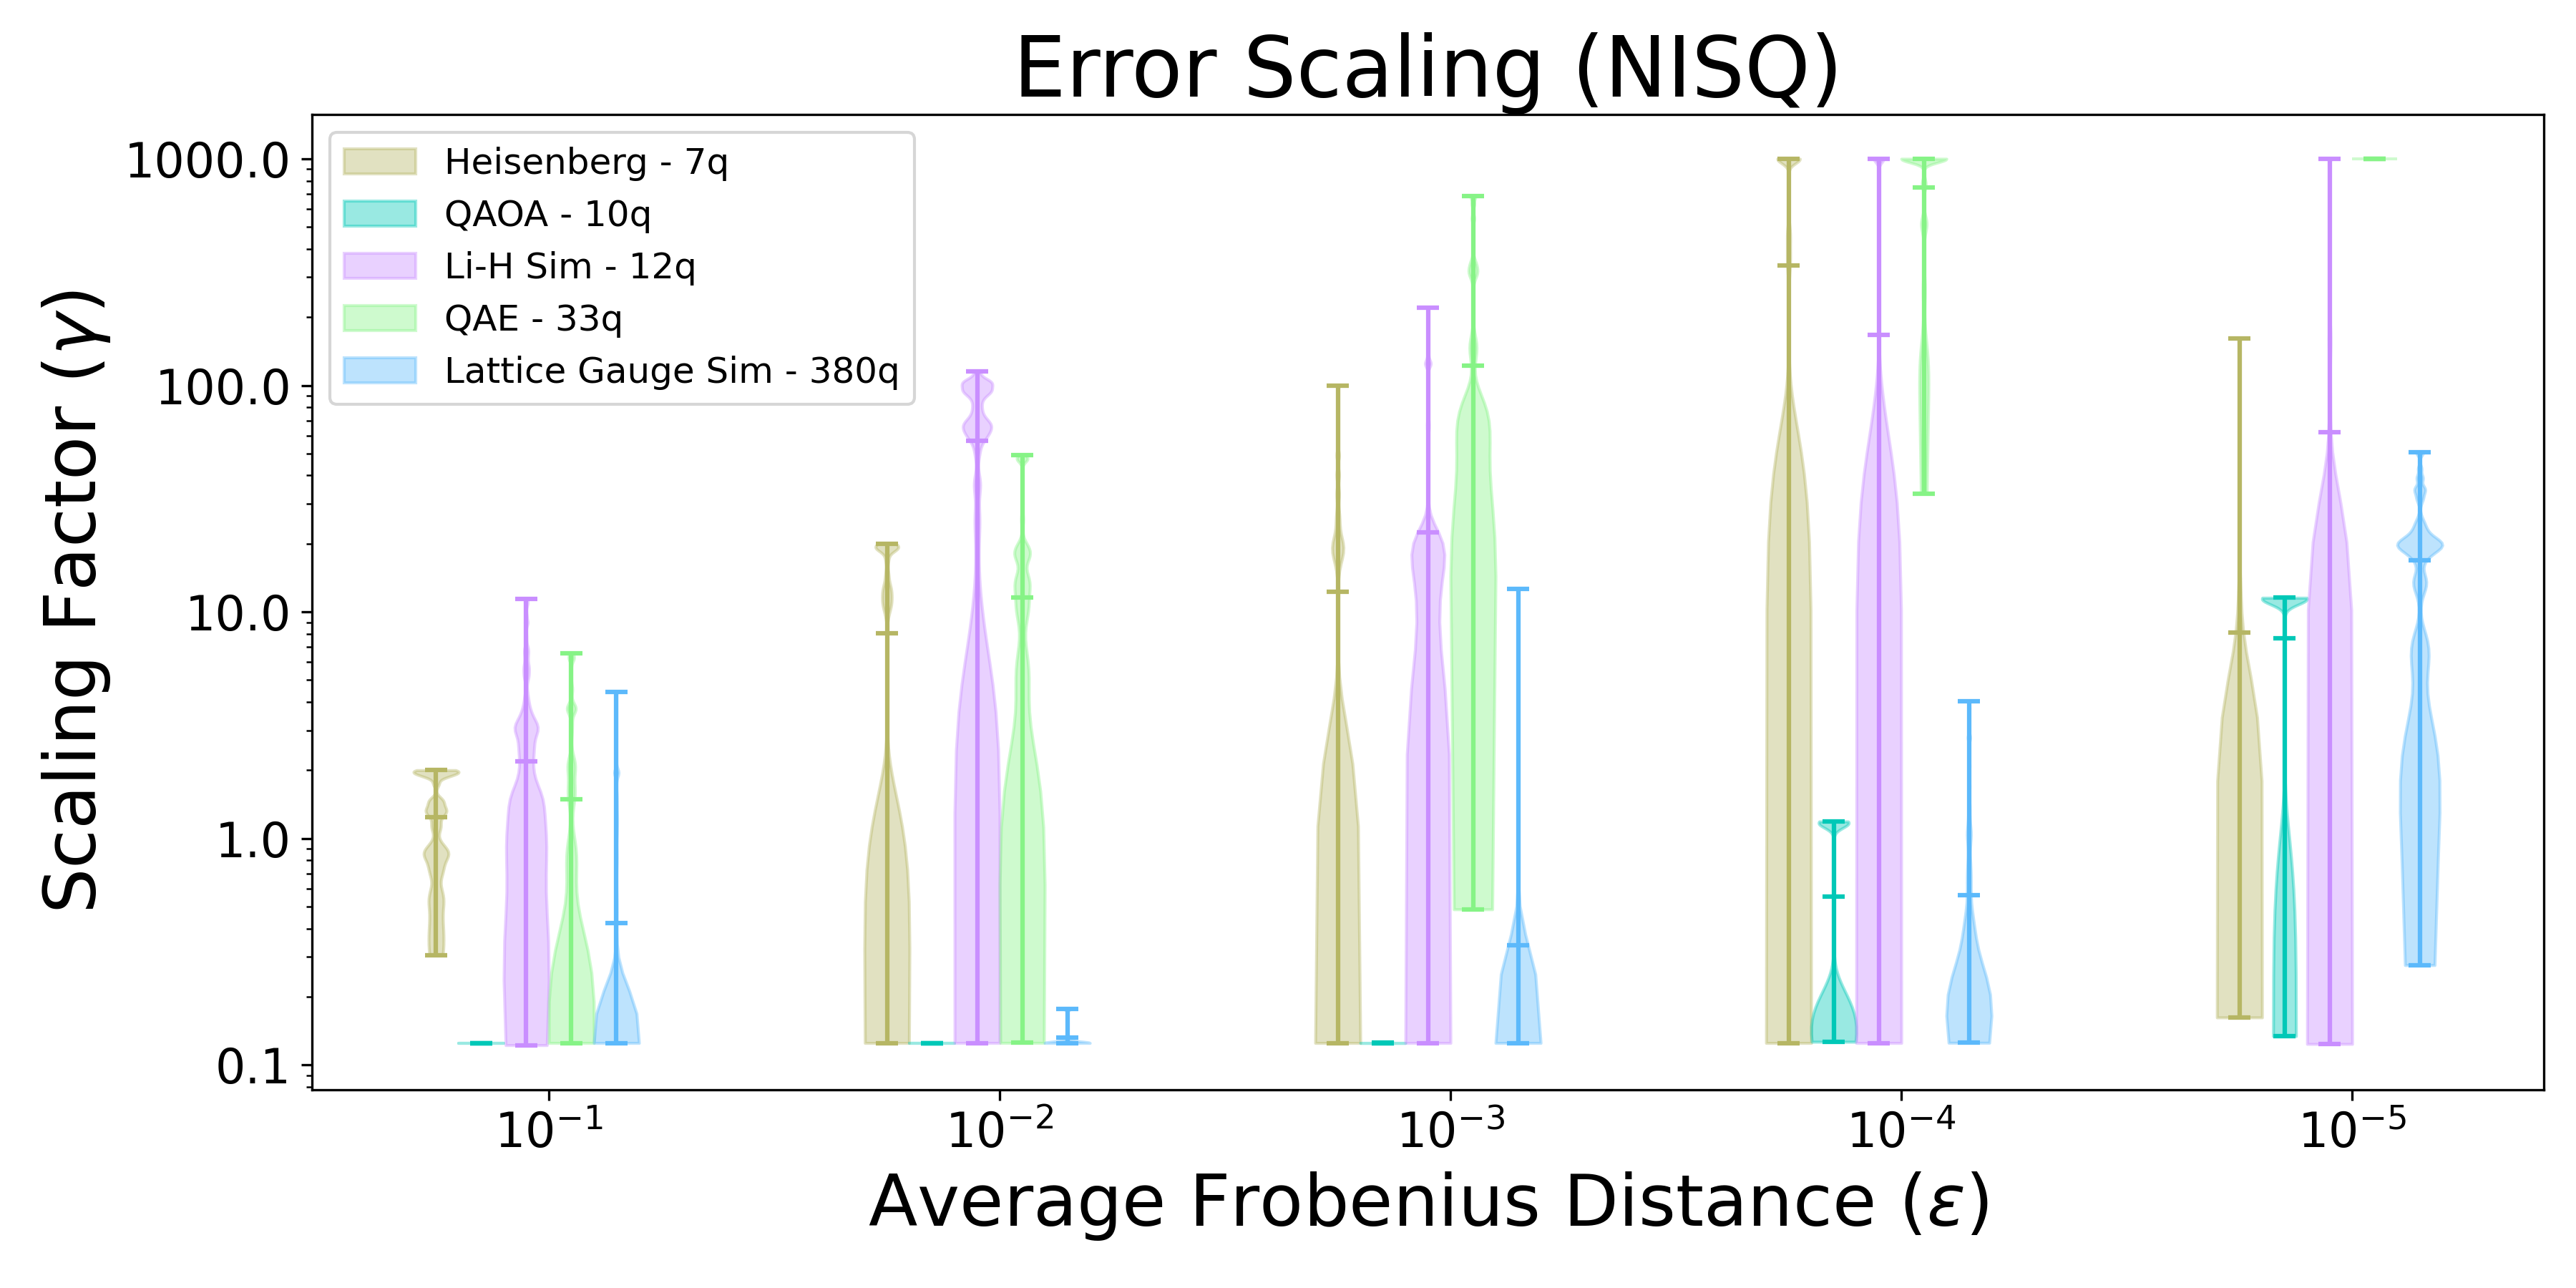
\includegraphics[width=\linewidth]{figures/supplementary/Error_scaling_final_nisq_20.png}
    \end{subfigure} \\
    \begin{subfigure}{0.7\textwidth}
        \centering
        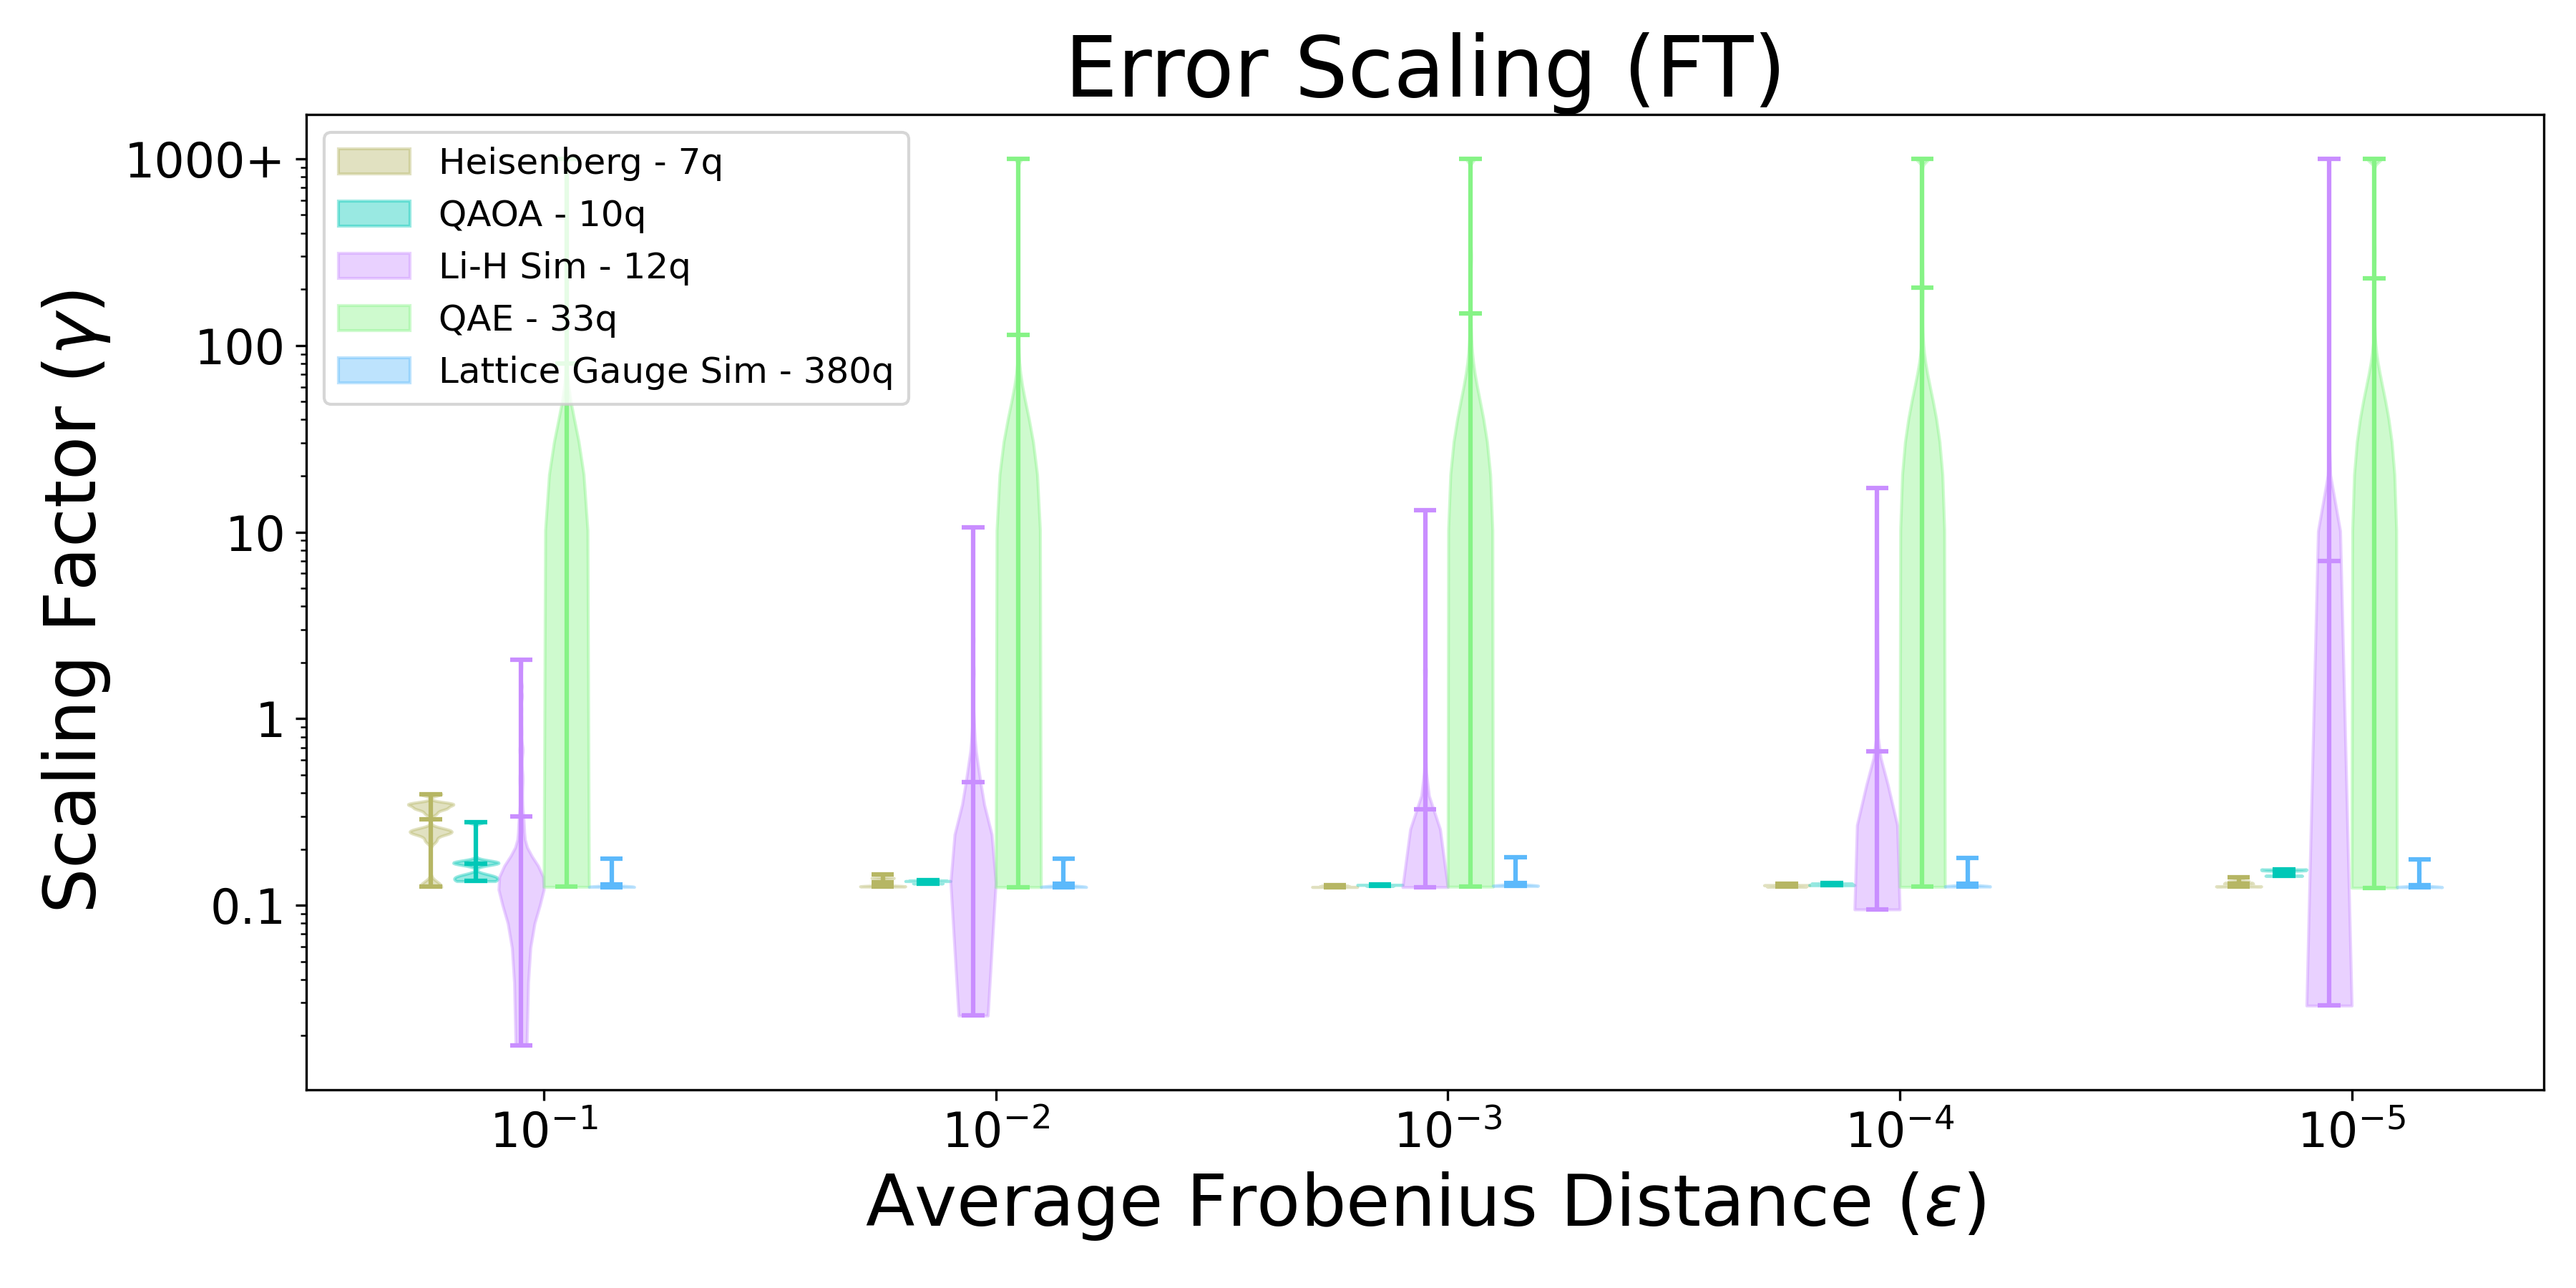
\includegraphics[width=\linewidth]{figures/supplementary/Error_scaling_final_cliff_20.png}
    \end{subfigure}
    \caption{Quadratic scaling factor $\gamma$ as a function of $\epsilon$, for some of the benchmarks.  
    Top: NISQ workflow (minimizing CNOT count).  
    Bottom: FT workflow (minimizing $T$-count).}
    \label{fig:error_scaling}
\end{figure*}


\begin{figure*}[t]
    \centering
    \begin{subfigure}{0.7\textwidth}
        \centering
        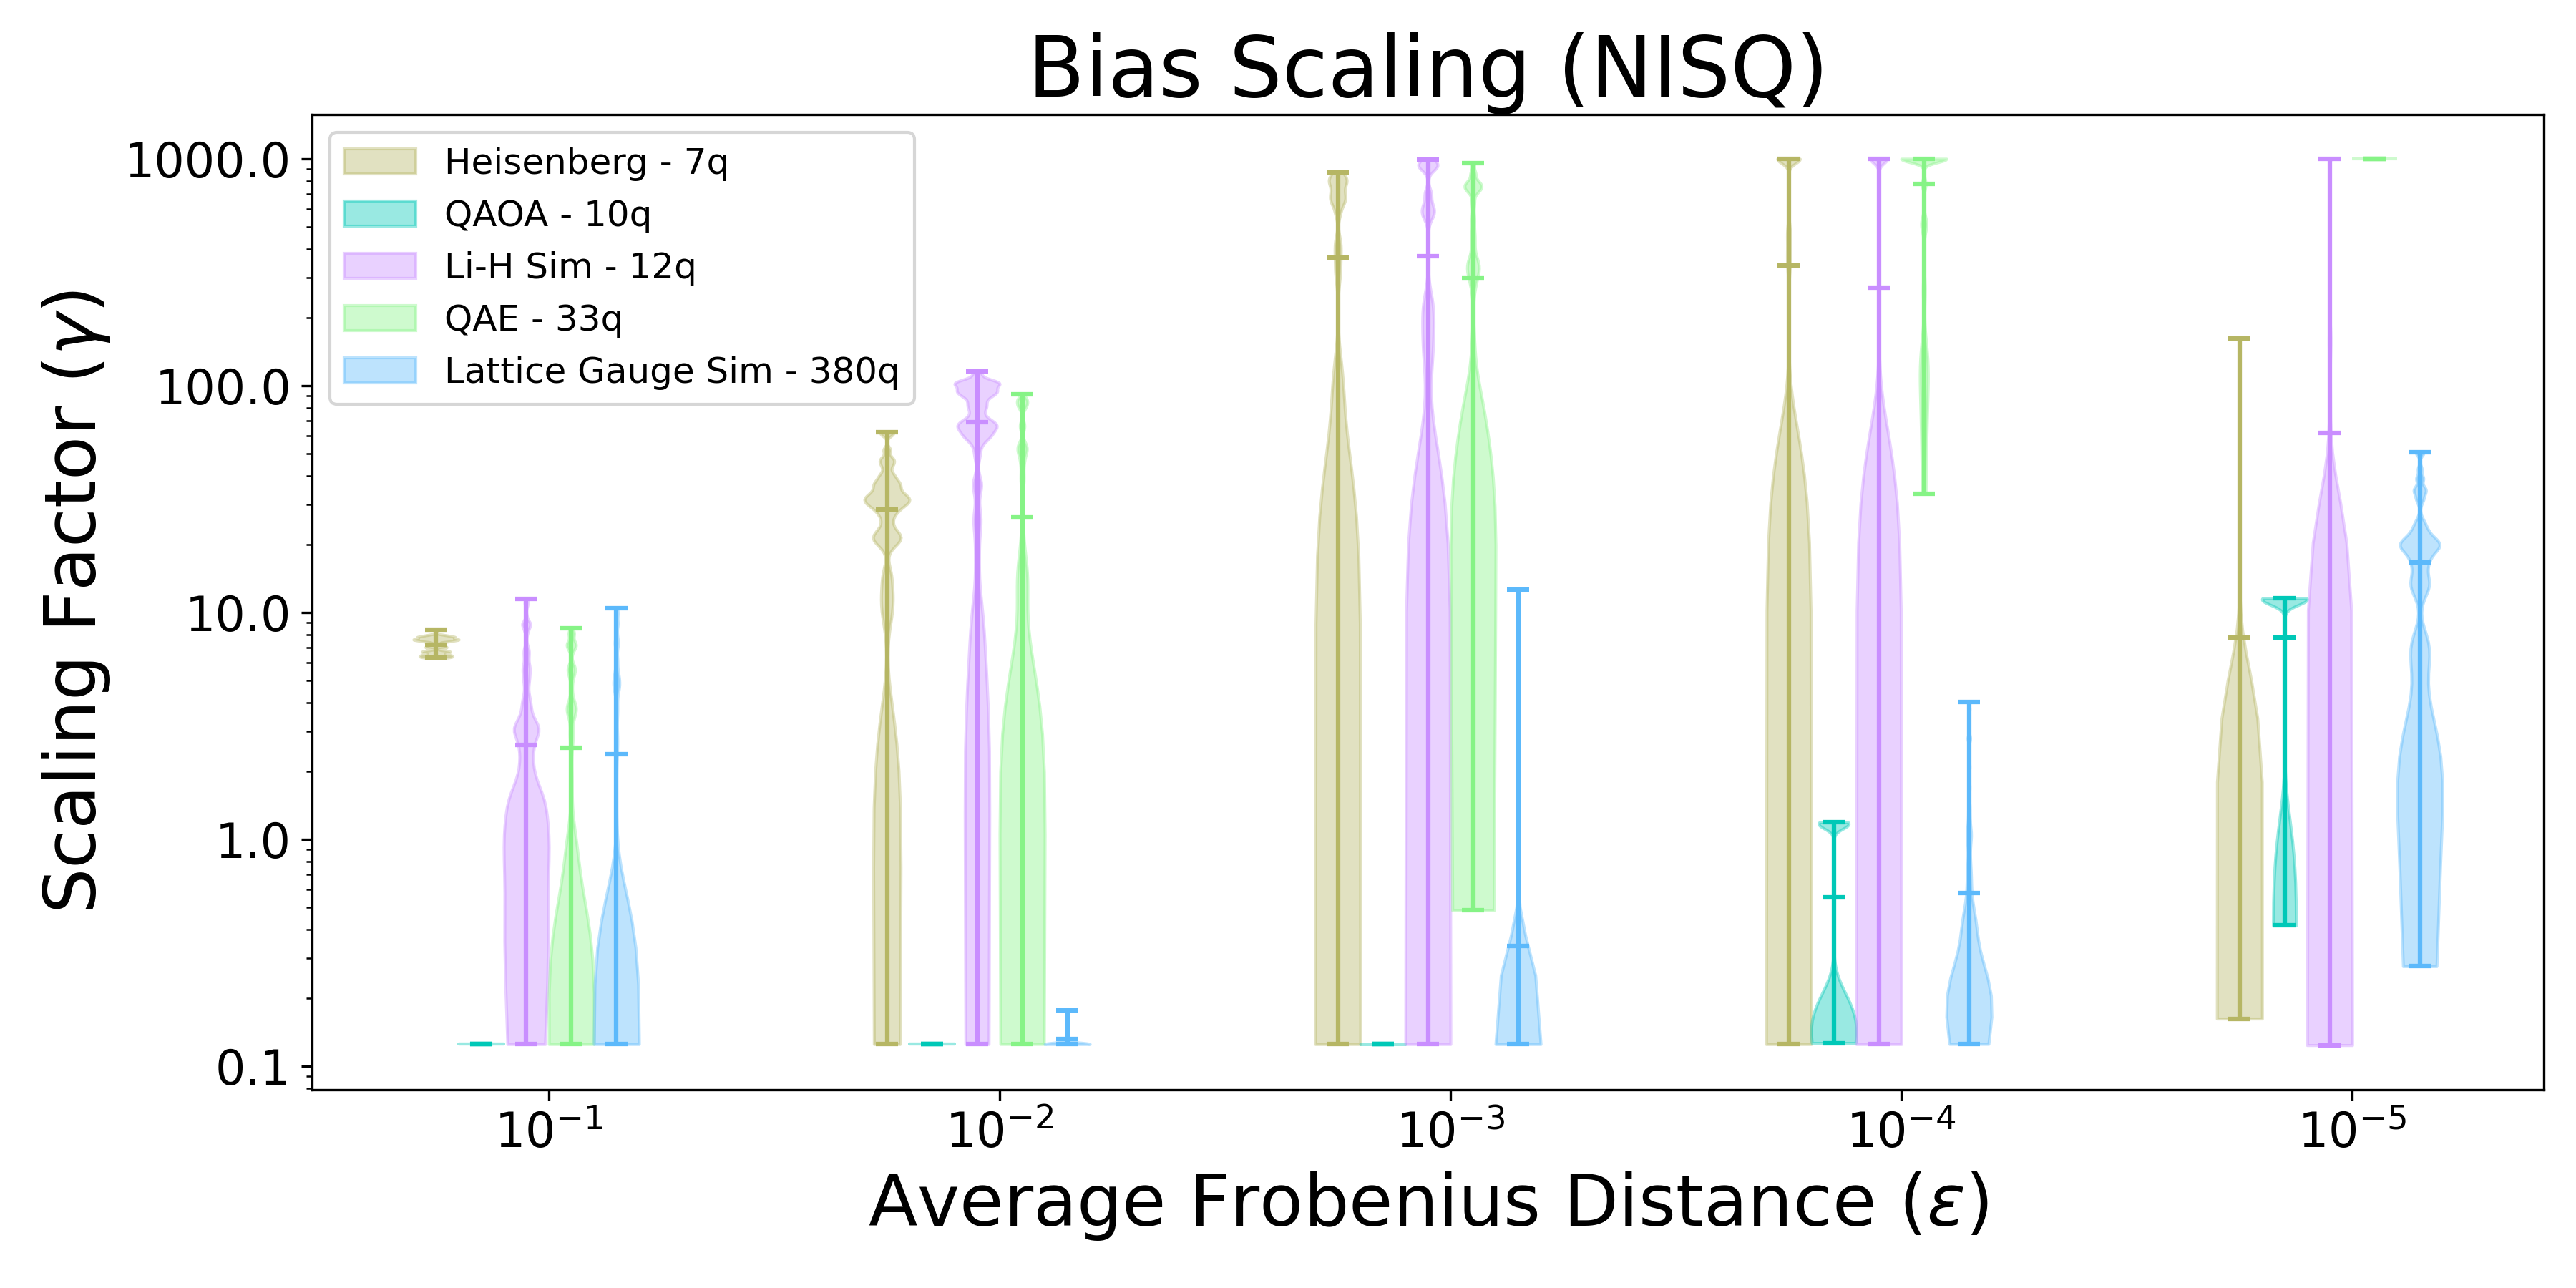
\includegraphics[width=\linewidth]{figures/supplementary/Bias_scaling_final_nisq_20.png}
    \end{subfigure} \\
    \begin{subfigure}{0.7\textwidth}
        \centering
        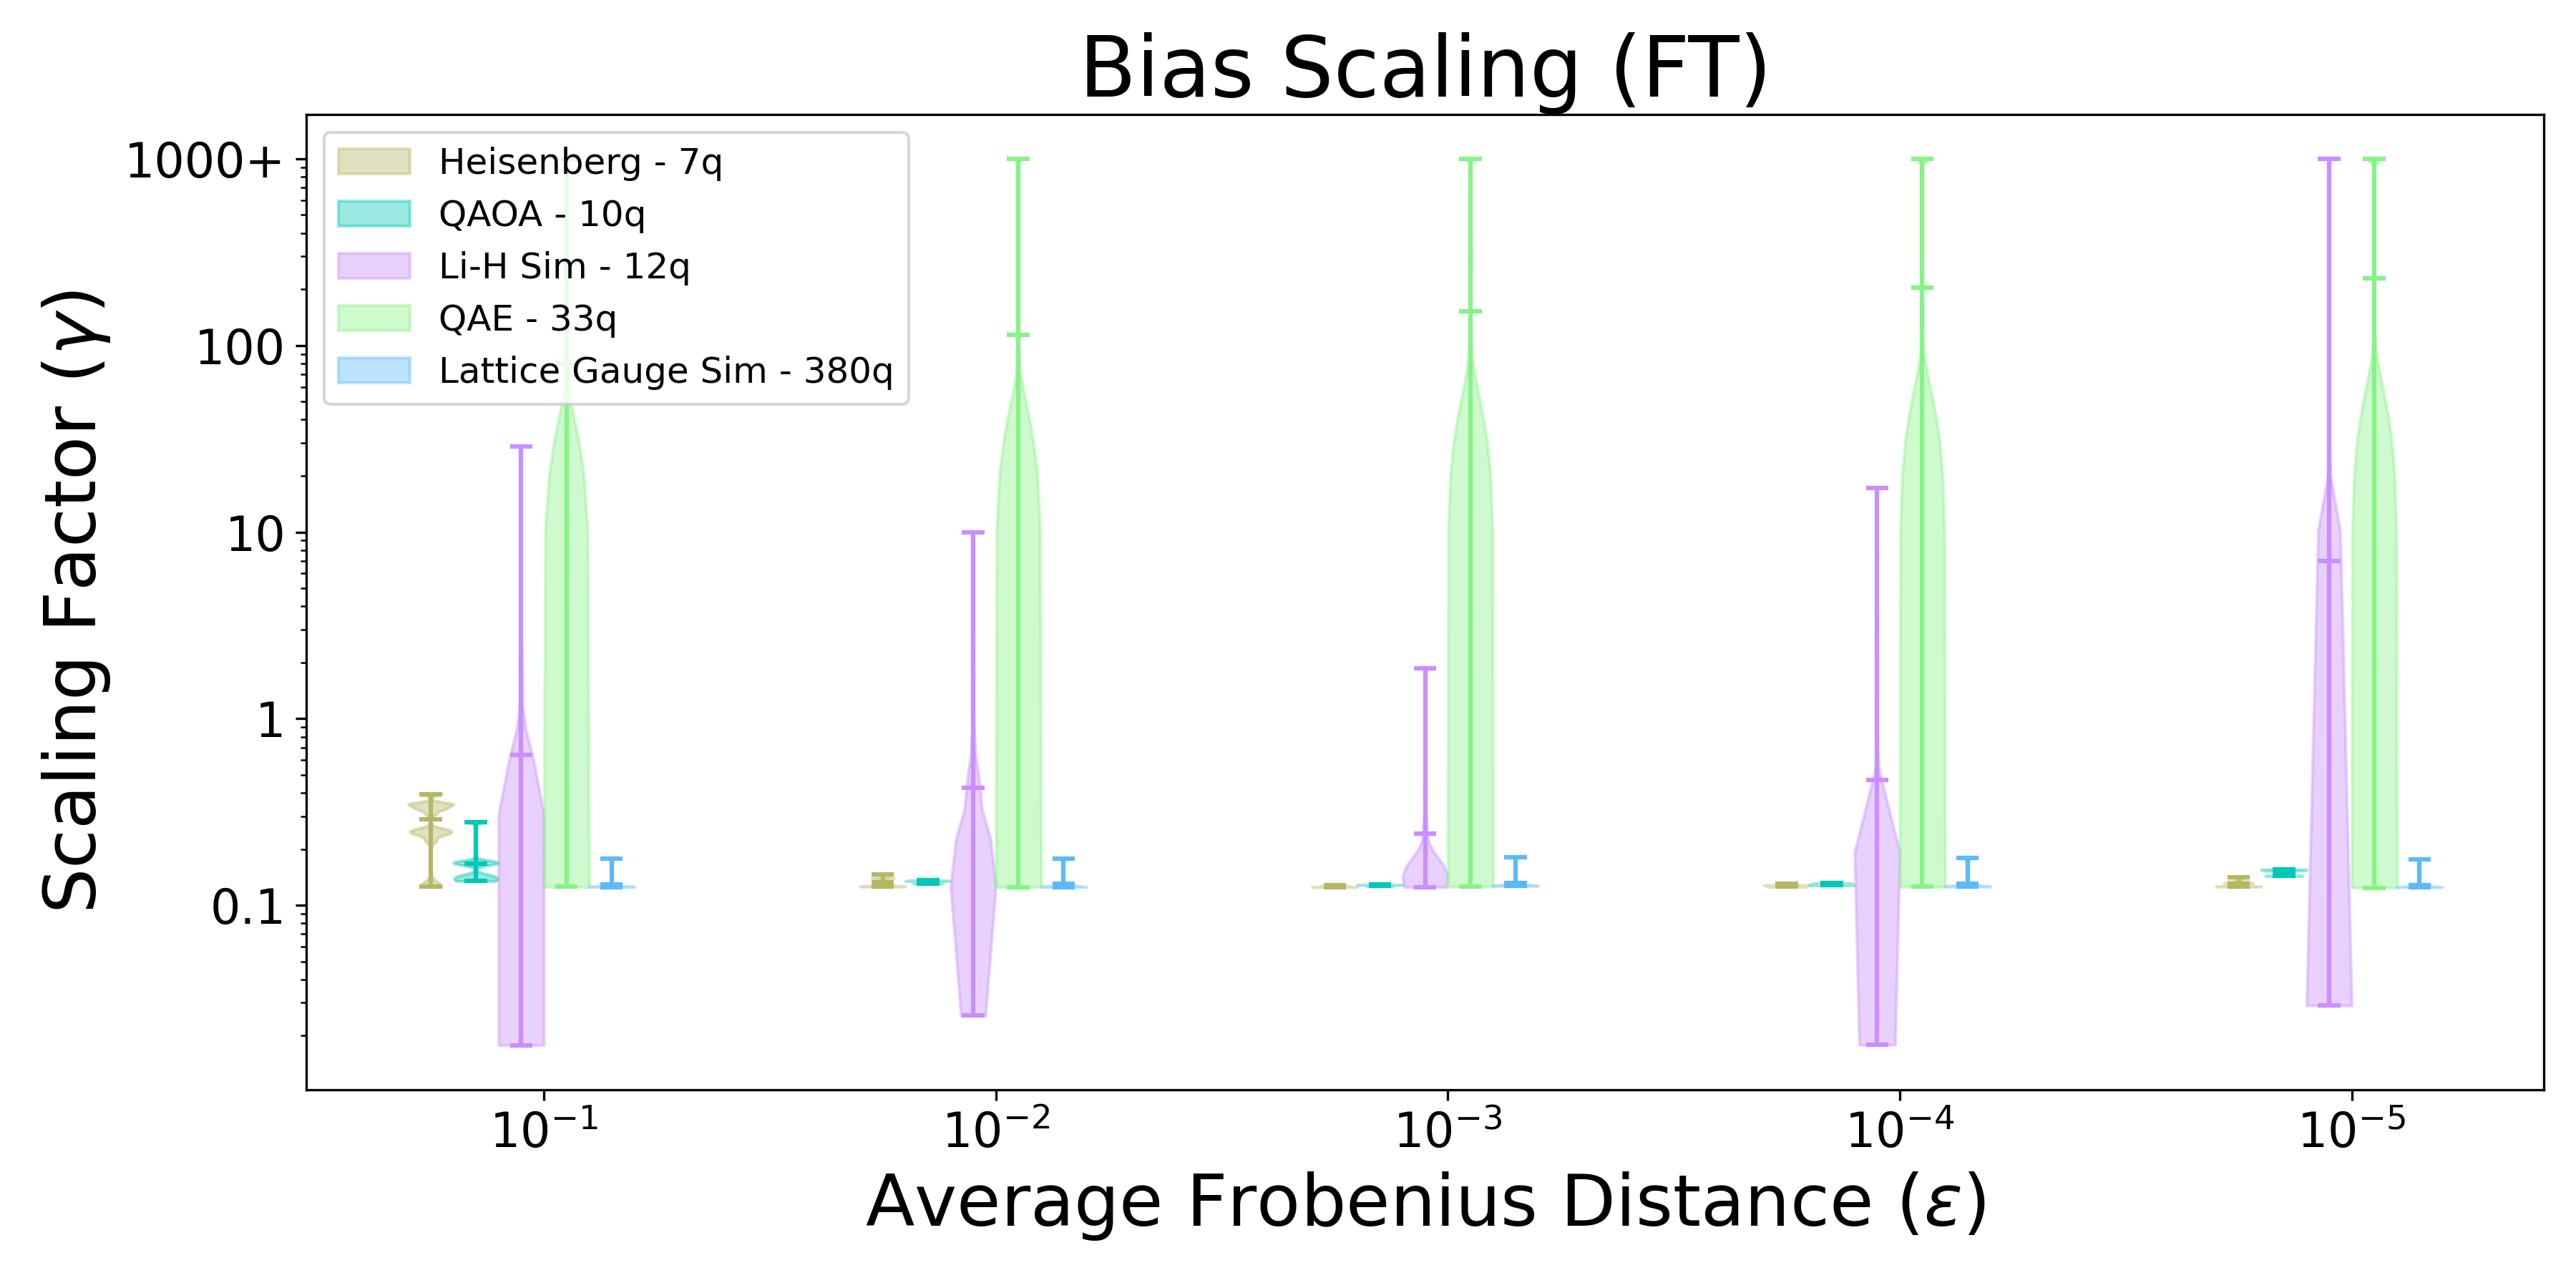
\includegraphics[width=\linewidth]{figures/supplementary/Bias_scaling_final_cliff_20.png}
    \end{subfigure}
    \caption{Quadratic scaling factor for the bias $\gamma_B$ as a function of $\epsilon$, for some of the benchmarks.  
    Top: NISQ workflow (minimizing CNOT count).  
    Bottom: FT workflow (minimizing $T$-count).}
    \label{fig:bias_scaling}
\end{figure*}

Figure \ref{fig:error_scaling} shows violin plots of the \emph{quadratic scaling factor} (QCF),  
\[
\gamma \equiv \frac{\normf{\sum_{i=1}^{M^\k} p^\k_i U^\k_i - V^\k}}{\epsilon^2},
\]  
for all blocks across many of our benchmarks.  
We expect $\gamma = O(1)$ when quadratic reduction of error is achieved.  
The plots indicate that, for most $\epsilon$ values, a significant subset of blocks in both NISQ and FT workflows achieve $O(\epsilon^2)$ scaling. In particular, almost all of the blocks in the FT workflow achieve $O(\epsilon^2)$ scaling. This is because we include a secondary compilation workflow, which trades off numerical synthesis resource reduction for improved scaling.

Our workflow does not require all blocks to satisfy Eq. \eqref{eq:wee_cond}. Blocks that fail to meet the condition are left unmodified, preserving the original circuit for those segments.  
This selective replacement explains why some benchmarks exhibit no gate count reduction (Tables 1 and 2 in the main text, particularly in the NISQ setting at small $\epsilon$). 

We also derived a sufficient condition for satisfying the ReWEE condition in terms of the bias of the compiler output,
\begin{align}
    \normf{\E{U} - V} < O(\epsilon^2).
\end{align}
We can define a quadratic scaling factor for the bias also, $\gamma_B \equiv \normf{\E{U}-V}/\epsilon^2$, and this quantity is displayed in Figure \ref{fig:bias_scaling} for all blocks of many of our benchmarks.


\section{Theoretical proofs}
In this section we provide proofs of Lemma 2 and Lemma 3 in the Methods section of the main text. Before restating the Lemmas and providing proofs, we recall several definitions from the main text.

$V$ is a target unitary on $n$ qubits, and $U_i$ are a set of approximate compilations of $V$ provided by a compiler. The compilation workflow can have probabilistic elements, and therefore we think of $U_i$ as independent, identically distributed (\emph{i.i.d.}) samples from some distribution of approximate compilations. The statistical properties we will demand of the compilation workflow are:
\begin{enumerate}
\item The compilations should all be close to the ideal, in the sense,
    \begin{align}
	\normf{U_i-V} \leq \epsilon, \quad \forall i		
		\label{eq:ass1}
	\end{align}
	\item The compilations have bounded variance, in the sense, $\E{U_i} \equiv \E{U}$ is independent of $i$, and
	\begin{align}
		\E{\normf{U_i - \E{U}}^2} \leq \epsilon', \quad \forall i
		\label{eq:ass2}
	\end{align}
\end{enumerate}
The expectations in these expressions and in the rest of this note are over the distribution of compilations generated by the compiler that satisfy Condition 1, \ie
$ \E{f(U)} = \int {\rm d}\mu_V(U) f(U), $
where ${\rm d}\mu_V(U)$ is the measure over $SU(2^n)$ defined by the compiler output that satisfies Condition 1 when the target is $V$ (the expectation symbol $\E{}$ should have a subscript $V$ but we omit this for ease). In addition,
\begin{enumerate}
    \item Define the channels $\mathcal{V}[\rho] = V \rho V\dg$, $\mathcal{U}_i[\rho] = U_i \rho U_i\dg$, and $\mathcal{U}[\rho] = \sum_i p_i U_i \rho U_i\dg$, for some probabilities $\{p_i\}$.
    \item $J_{\mathcal{E}} \equiv \sum_{i,j=1}^d \mathcal{E}(\ket{i}\bra{j})\otimes \ket{i}\bra{j}$ is the Choi matrix representation of the channel $\mathcal{E}$, which we assume to be acting acting on $d\times d$ density matrices and outputting density matrices of the same size.
\end{enumerate}

\noindent \emph{\bf Lemma 2:} \emph{Let $V$ and $U_i$ be defined as above. Given probabilities $\{p_i\}_{i=1}^M$, ($\sum_{i=1}^M p_i=1$), a sufficient condition for achieving $\E{\normf{\sum_{i=1}^M p_i U_i - V}} \leq O(\epsilon^2)$ is the \emph{reduced bias condition}: $\normf{\E{U}-V} \leq O(\epsilon^2)$.}

\noindent \textit{Proof:} First, note that $\E{\normf{\sum_{i=1}^M p_i U_i - V}} \leq O(\epsilon^2)$ follows directly from $\E{\normf{\sum_{i=1}^M p_i U_i - V}^2} \leq O(\epsilon^4)$ through an application of Jensen's inequality, and so we prove the latter statement.
\begin{align}
    \E{\normf{\sum_{i=1}^M p_i U_i - V}^2} & \leq \E{\normf{\frac{1}{M}\sum_{i=1}^M U_i - V}^2} 
	   = \normf{\overline{bias}}^2 + \frac{1}{M}\overline{var} + \left(1-\frac{1}{M}\right)\overline{covar}, 
       \label{eq:b-v-c} 
\end{align}
where,
\begin{align}
	\overline{bias} &= (\E{U} - V) \label{eq:bias} \\
	\overline{var} &= \frac{1}{M}\sum_{i=1}^{M} \E{\normf{U_i - \E{U}}^2} \label{eq:var} \\
	\overline{covar} &= \frac{1}{M(M-1)}\sum_{i=1}^M \sum_{j \neq i}^M \mathbb{E} \left\{ \tr[(U_i-\E{U})\dg \cdot (U_j - \E{U})] \right\} 
    \label{eq:covar}
\end{align}
The first inequality follows from the fact that the weights $p_i$ are optimized to reduce the ensemble error. The equality on the second line follows from using the definition of the Frobenius norm to decompose the quantity of interest in a \emph{bias-variance-covariance} decomposition, a well-known decomposition of generalization error of ensembles of estimators in machine learning \cite{Ueda_1996, Brown_20005}. Here, $\overline{bias}$ is the bias of the (uniform) ensemble, $\overline{var}$ is the (sample) average of the variance of the members of the ensemble, and $\overline{covar}$ is the covariance of the ensemble members. Since the ensemble members are sampled \emph{i.i.d.} from the compiler output distribution, the covariance term is zero. In addition, using the fact that the samples have bounded variance, Eq. \eqref{eq:ass2}, we get
$\E{\normf{\sum_{i=1}^M p_i U_i - V}^2} \leq \normf{\E{U}-V}^2 + \frac{\epsilon'}{M}$.
This quantity can be bounded as $O(\epsilon^4)$ by satisfying the reduced bias condition and choosing $M \geq \epsilon'/\epsilon^4$. \QED
\\

\noindent \emph{\bf Lemma 3:} \emph{Let $V$ and $U_i$ be defined as above, and let these unitaries act on a register of $n$ qubits; \ie ${\rm dim}~ V = {\rm dim}~ U_i = 2^n \equiv d$. Define $\mathcal{V}[\rho] = V \rho V^{\dagger}$ as a target channel, and $\mathcal{U}[\rho] = \sum_{i=1}^M p_i U_i \rho U_i\dg$ as an optimized ensemble channel, such that $d_\diamond(\mathcal{V}, \mathcal{U})\leq O(\epsilon^2)$. Further, let $\hat{\mathcal{U}}[\rho] = \frac{1}{T}\sum_{i=1}^T U_{\sigma(i)} \rho U_{\sigma(i)}\dg$ be the empirical channel defined by sampling and averaging over $U_i$ according to the distribution $\{p_i\}$ -- \ie $\sigma(i) \in \{1,...,M\}$. For $\epsilon, \delta \in (0,1)$, $\pr\left\{ d_\diamond(\mathcal{V}, \hat{\mathcal{U}}_T) \leq O(\epsilon^2) \right\} > 1-\delta$, given
\begin{align}
    T \geq \frac{2v + \frac{2}{3}R \left(\epsilon^2/(2d^2)\right) }{\left(\epsilon^2/(2d^2)\right)^2}\log \frac{2d^2}{\delta}
    \label{eq:T_bound}
\end{align}
Here, $v \equiv \normo{\sum_{i=1}^M p_i (J_i - J_{\mathcal{U}})^2}, R \equiv \max_i \normo{J_i - J_{\mathcal{U}}}$, and $J_i (and J_{\mathcal{U}}$) are the $d^2$-dimensional Choi matrices associated to the channel $\mathcal{U}_i[\rho] = U_i \rho U_i^{\dagger}$ (and $\mathcal{U}$).}

\noindent \textit{Proof:} We begin by an application of the triangle inequality:
\begin{align}
    d_\diamond(\mathcal{V}, \hat{\mathcal{U}}) &\leq  d_\diamond(\mathcal{V}, \mathcal{U}) +  d_\diamond(\mathcal{U}, \hat{\mathcal{U}}) \nn \\  
    & = O(\epsilon^2) + d_\diamond(\mathcal{U}, \hat{\mathcal{U}}),
    \label{eq:lemma3_1}
\end{align}
and hence we are left with the task of determining the sample size $T$ necessary to satisfy $d_\diamond(\mathcal{U}, \hat{\mathcal{U}}) \leq \epsilon^2$. Therefore, 
\begin{align}
    d_\diamond(\mathcal{U}, \hat{\mathcal{U}}) &\equiv \normd{\mathcal{U}- \hat{\mathcal{U}}} \nn \\
    & \leq \normt{J_\mathcal{U} - J_{\hat{\mathcal{U}}}} \nn \\
    & \leq 2d^2 \normo{J_\mathcal{U} - J_{\hat{\mathcal{U}}}},
\end{align}
where the first inequality follows from an identity established by Watrous \cite[Exercise 3.6]{watrous_2018}, the second is the application of a standard norm inequality ($\normt{A}\leq {\rm rank}(A)\normo{A}$), and an overestimate of the relevant rank: ${\rm rank}(J_\mathcal{U} - J_{\hat{\mathcal{U}}}) \leq {\rm rank}(J_\mathcal{U} ) + {\rm rank}(J_{\hat{\mathcal{U}}}) \leq 2d^2$. In the above, the Choi matrices are explicitly, $J_\mathcal{U} = \sum_{i=1}^M p_i J_i$ and $J_{\hat{\mathcal{U}}} = \frac{1}{T} \sum_{i=1}^T J_i$, with $J_i \equiv J_{\mathcal{U}_i}$. 

Now that the error is expressed in terms of an operator norm, we can apply standard Bernstein matrix concentration inequality \cite{tropp_2015} to get, 
\begin{align}
    \pr\left\{ d_\diamond(\mathcal{U}, \hat{\mathcal{U}}) \geq \epsilon^2 \right\} \leq \pr\left\{ \normo{J_\mathcal{U} - J_{\hat{\mathcal{U}}}} \geq \frac{\epsilon^2}{2d^2} \right\} \leq 2d^2 \exp\left(-\frac{T(\frac{\epsilon^2}{2d^2})^2}{2v + \frac{2}{3}R \frac{\epsilon^2}{2d^2}}\right),
\end{align} 
where $v$ and $R$ are the variance and maximum deviation as defined in the Lemma statement. In order for the right-hand side to be at most $\delta$, the sample size given in Eq. \eqref{eq:T_bound} is sufficient. Finally, combining this with the statement in Eq. \eqref{eq:lemma3_1} yields the Lemma statement. 
\QED

\subsection{Statistics of factors entering sample complexity}
While the formal sample complexity bound in Lemma 3 scales with $\epsilon$ as $O(1/\epsilon^4)$, in the main text we claimed that in practice, $v=O(\epsilon^2)$, and therefore, the number of samples needed is $O(1/\epsilon^2)$. Figure 5 in the main text provided evidence for this gentler scaling for one of the benchmarks in our study. While Lemma 3 is stated in terms of diamond distance between the empirical channel and the ensemble channel, this error is infeasible to evaluate numerically because of the difficulty of calculating the diamond distance for channels acting on many qubits. Therefore, in Figure 5 of the main text, we showed the trace distance error in the output, $\normt{\rho_{T} - \rho_i}$,
where $\rho = \sum_{i=1}^M p_i U_i \rho_{0} U_i\dg$ is the output of the ensemble channel for random input state $\rho_{0}$, and $\rho_{T} = \frac{1}{T}\sum_{i=1}^T U_i \rho_{0} U_i\dg$ is the output of the empirical channel for the same input (the $U_i$ in the empirical channel are sampled according to the distribution $\{p_i\}$ set by the ensemble channel). 

The equivalent sample complexity bound for this error metric is $\pr\{\normt{\rho_{T} - \rho} \geq \epsilon^2\} \leq 1-\delta$, if
\begin{align}
    T \geq \frac{2v + \frac{2}{3}R \left(\epsilon^2/(2d)\right) }{\left(\epsilon^2/(2d)\right)^2}\log \frac{2d}{\delta},
    \label{eq:T_bound_state} 
\end{align}
where $v \equiv \normo{\sum_{i=1}^M p_i (\rho_i - \rho)^2}, R \equiv \max_i \normo{\rho_i - \rho}$, and $\rho_i = U_i\rho_0 U_i\dg$. Calculating the values $v$ and $R$ is difficult for most of the benchmarks we studied, even in this case, because $M$ can be very large for full circuits, and thus computing the ideal ensemble output $\rho$ is numerically intensive. Instead, we compute these variance and maximum deviation values, $v$ and $R$, for all blocks in two of our benchmark circuit ensembles. As shown in Fig. \ref{fig:vR}, $v \ll \epsilon^2$ in practice, which explains the gentler scaling of $T$ required to approximate the ensemble channel with the empirical channel.

\begin{figure*}[ht]
    \centering
        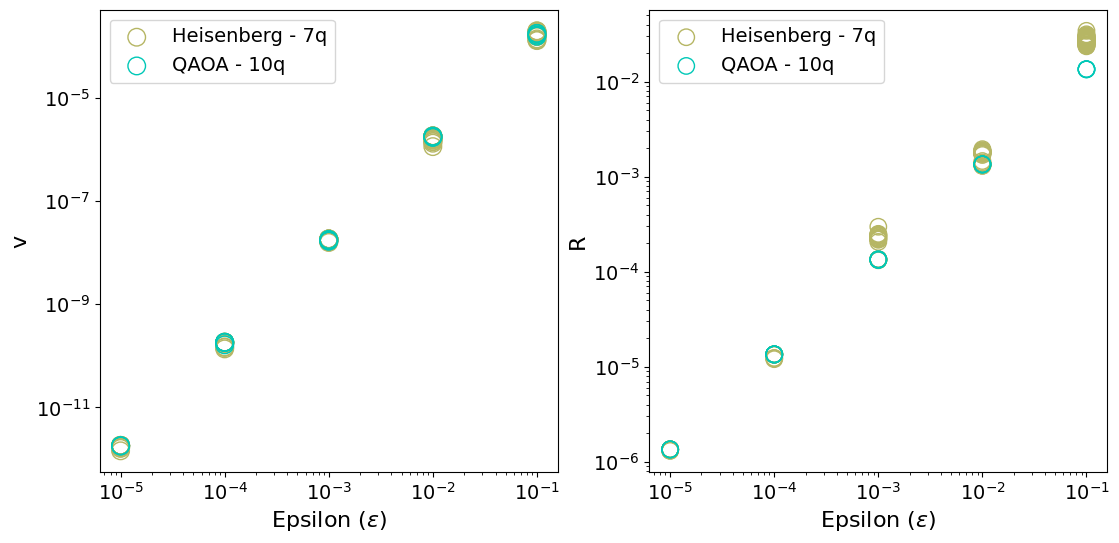
\includegraphics[width=0.7\linewidth]{figures/supplementary/v_R_all_circs_1_final.png}
    \caption{Values of variance and maximum deviation factors, $v$ and $R$, entering the sample complexity bound Eq. \eqref{eq:T_bound_state} for each block of two benchmark circuits.}
    \label{fig:vR}
\end{figure*}

\newpage

\documentclass[fleqn,10pt]{wlscirep}
\usepackage[utf8]{inputenc}
\usepackage[T1]{fontenc}
\usepackage{wrapfig}
\usepackage{subcaption}
\usepackage{multirow}
\usepackage{multicol}
\usepackage{tikz}
\usepackage{graphicx}
\usepackage{standalone}

\newcommand{\eg}{\emph{e.g.,~}}
\newcommand{\ie}{\emph{i.e.,~}}
\newcommand{\bx}{\mathbf{x}}
\newcommand{\by}{\mathbf{y}}
\newcommand{\bp}{\mathbf{p}}
\newcommand{\hx}{\hat{x}}
\newcommand{\hp}{\hat{p}}
\newcommand{\ket}[1]{\vert#1\rangle}
\newcommand{\bra}[1]{\langle #1\vert}
\newcommand{\expect}[1]{\langle #1\rangle}
\newcommand{\dg}{^\dagger}
\newcommand{\nn}{\nonumber}
\newcommand{\pr}{{\rm Pr}}

\newcommand{\normf}[1]{\left\lVert #1 \right\rVert_F}
\newcommand{\normo}[1]{\left\lVert #1 \right\rVert}
\newcommand{\normt}[1]{\left\lVert #1 \right\rVert_1}
\newcommand{\normd}[1]{\left\lVert #1 \right\rVert_\diamond}
\newcommand{\E}[1]{\mathbb{E}\left\{ #1 \right\}}

\newcommand{\tr}{{\rm tr}}
\renewcommand{\k}{{(k)}}
\newcommand{\p}{{\bf\sf p}}
\newcommand{\braket}[2]{\langle #1 \vert #2 \rangle}

\newcommand*{\QED}{\null\nobreak\hfill\ensuremath{\blacksquare}}%

\makeatletter
\renewcommand{\@maketitle}{%
{%
\thispagestyle{empty}%
\vskip-36pt%
{\raggedright\sffamily\bfseries\fontsize{20}{25}\selectfont \@title\par}%
\vskip10pt
{\raggedright\sffamily\fontsize{12}{16}\selectfont  \@author\par}
\vskip25pt%
}%
}%
\makeatother

\newcommand{\red}[1]{{\color{red}#1}} 
\newcommand{\needcite}{{\color{red}[XX]~}}
\long\def\comment#1{}
\long\def\note#1{{\em #1 }}
\def\parah#1{\vspace*{0.0in} \noindent{\bf #1:}}

\title{Supplementary Information for: Application Scale Quantum Circuit Compilation with Controlled Error}

\author[1,2,*]{Justin Kalloor}
\author[3]{Lucas Kovalsky}
\author[1,2]{Mathias Weiden}
\author[2]{John Kubiatowicz}
\author[1]{Ed Younis}
\author[1]{Costin Iancu}
\author[3,+]{Mohan Sarovar}
\affil[1]{Computational Research Division, Lawrence Berkeley National Laboratory, Berkeley, CA, 94702, USA}
\affil[2]{Department of Electrical Engineering and Computer Science, University of California, Berkeley, CA, 94702, USA}
\affil[3]{Quantum Algorithms and Applications Collaboratory, Sandia National Laboratories, Livermore, CA, 94550, USA}

\affil[*]{jkalloor3@berkeley.edu}
\affil[+]{mnsarov@sandia.gov}



\begin{document}

\flushbottom
\maketitle

\section{Description of benchmark applications and circuits}
For our benchmarks, we use a variety of quantum algorithms across different domains of interest.

\subsection*{Hamiltonian Simulation Algorithms}
\begin{enumerate}
    \item \textbf{SU(2) Lattice Gague Simulation} - We follow the construction outlined in the paper by Rahman et. al \cite{rahman_2022} to simulate the motion of an excitation on a spatial lattice.
    \item \textbf{Li-H Molecule} - We simulate the electronic energy of a Lithium Hydride molecule. The circuit was generated using the Qiskit Nature and PySCF\cite{qiskit} libraries. The fermionic operator was mapped to qubits using a Jordan Wigner mapper\cite{jordan_wigner}. When calculating the observable, we use the Hartree Fock \cite{hartree_fock} state as the initial state.
    \item \textbf{Fermi-Hubbard Model} We run the Fermi-Hubbard model on a square lattice with periodic boundary conditions. The lattice has uniform interaction energies as well as a uniform onsite potential and was mapped to a quantum circuit with a Jordan Wigner mapper. For the observable calculations, we pass in the ground state of the non-interacting model as the initial state.
    \item \textbf{Heisenberg Model} - We simulate the nearest neighbor Heisenberg model with the Hamiltonian defined as:
    \[H = J \cdot \sum{X_iX_{i+1} + Y_iY_{i+1} + Z_iZ_{i+1}}\] and use the all zero state as the initial ground state.
\end{enumerate}

\subsection*{Arithmetic Sub-Modules}

\begin{enumerate}
    \item \textbf{Multiplier} - A quantum sub-circuit to multiply two registers and store into an output register\cite{qiskit}.
    \item \textbf{Adder} - A simple implementation of a Ripple-Carry Adder to add together two quantum registers \cite{qiskit}.
    \item \textbf{QFT Adder} - An implementation of the Draper QFT Adder \cite{draper}.
\end{enumerate}

\subsection*{Quantum Sub-Routines}

\begin{enumerate}
    \item \textbf{Quantum Amplitude Estimation (QAE)} - An implementation of the quantum amplitude estimation circuit on a Bernoulli Operator with a probability of 0.5 \cite{qiskit, brassard}.
    \item \textbf{Quantum Phase Estimation (QPE)} - We estimate the phase of a randomly generated circuit. In our 14 qubit example, we generate a 7-qubit random circuit, and use 7 qubits for precision.
\end{enumerate}

\subsection*{Quantum Optimization}

\begin{enumerate}
    \item Quantum Approximate Optimization Algorithm - An implementation of the optimization circuit given in QASMBench\cite{qasm_bench}.
\end{enumerate}

\section{``Rigid" Circuit Blocks}
\label{sec:rigid_blocks}
As ensemble generation time grows exponentially with the number of qubits, circuit partitioning allows us to scale our workflow to application-width circuits. We first split our circuit into blocks of width $w$, and then generate a block-level ensemble for each partition \emph{in parallel}. Importantly, we are able to accept/reject each ensemble based on the ReWEE condition, which gives us additional flexibility on which circuits benefit from our methodology. We do not need a perfect ensemble for the circuit as a whole; we can pick and choose which parts of the circuit benefit from approximation.

Despite this additional freedom provided by the partitioner, there are benchmarks that are unable to see any reduction in the NISQ compilation workflow. This happens when the input circuit is partitioned into ``rigid" blocks. Rigid blocks are circuits (along with their underlying unitaries) that either 1) Cannot be reduced (e.g no CNOTs can be removed without significant approximation error or 2) Only have a few approximate solutions, which are not diverse enough to form a convex hull around the original unitary.

\begin{figure}[htbp]
\centering
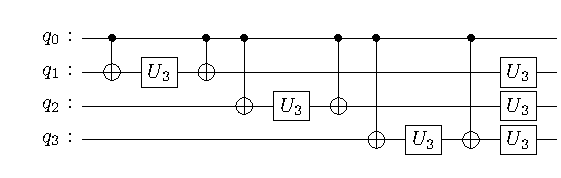
\includegraphics[width=0.55\textwidth]{figures/supplementary/rigid_block_one.pdf} \\
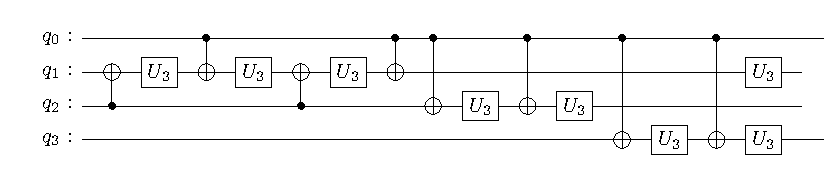
\includegraphics[width=0.8\textwidth]{figures/supplementary/rigid_block_two.pdf}
\caption{Two examples of ``rigid" circuit blocks from the QFT Adder circuit and QPE circuit.}
\label{fig:rigid_blocks}
\end{figure}

Figure \ref{fig:rigid_blocks} illustrates two examples of these rigid structures. The first block is from the QFT Adder circuit while the second block is from a QPE circuit. The first circuit contains 3 consecutive controlled rotations with the same control qubit (q0), while the second circuit contains a multi-controlled rotation and two controlled rotations. Consecutive rotations with a only a few control qubits prove difficult to reduce in the NISQ setting, since the removal of any single CNOT adds significant error to the underlying unitary. On top of that, since the control qubit is being constantly reused, it is hard to find approximate ``shortcuts" by leveraging CNOTs on surrounding qubits.

For the demonstration of our workflow shown in this work, we use a block size of $4$, while the standard BQSKit compile width is $3$. We found that by increasing the block size, both the reduction quality and probability of finding a convex hull improved, as the partitions were more likely to have many control and target qubits and be less rigid. We predict that increasing the block size to larger and larger sizes would continue to improve our results, albeit at the cost of compilation time.




\section{Statistics of ensemble error reduction}
\label{sec:error_scaling}

The benefits of using an ensemble channel are guaranteed only if the ReWEE condition is satisfied, \ie the weighted ensemble error is quadratically reduced, 
\begin{align}
    \normf{\sum_{i=1}^{M^\k} p^\k_i U^\k_i - V^\k} \leq O(\epsilon^2), 
\label{eq:wee_cond}
\end{align}
when each compilation, $U^\k_i$, is performed to error $\epsilon$.  
In practice, it is challenging to construct an ensemble of approximate circuits that both:  
\begin{enumerate}
    \item Uses fewer resource-intensive gates (e.g., CNOT or $T$ gates) on average than the original circuit, and  
    \item Satisfies Eq. \eqref{eq:wee_cond}.  
\end{enumerate}  
While explicit algorithms exist for guaranteeing Eq. \eqref{eq:wee_cond} \cite{PhysRevA.95.042306}, they are difficult to scale to multi-qubit circuits and do not provide resource efficiency guarantees.

In the main text we have shown that both criteria can be met for several of the benchmarks we studied.   
Here, we present statistics that explain how this is achieved through quadratic reduction in the weighted ensemble error and selective filtering of circuit blocks.



\begin{figure*}[t]
    \centering
    \begin{subfigure}{0.7\textwidth}
        \centering
        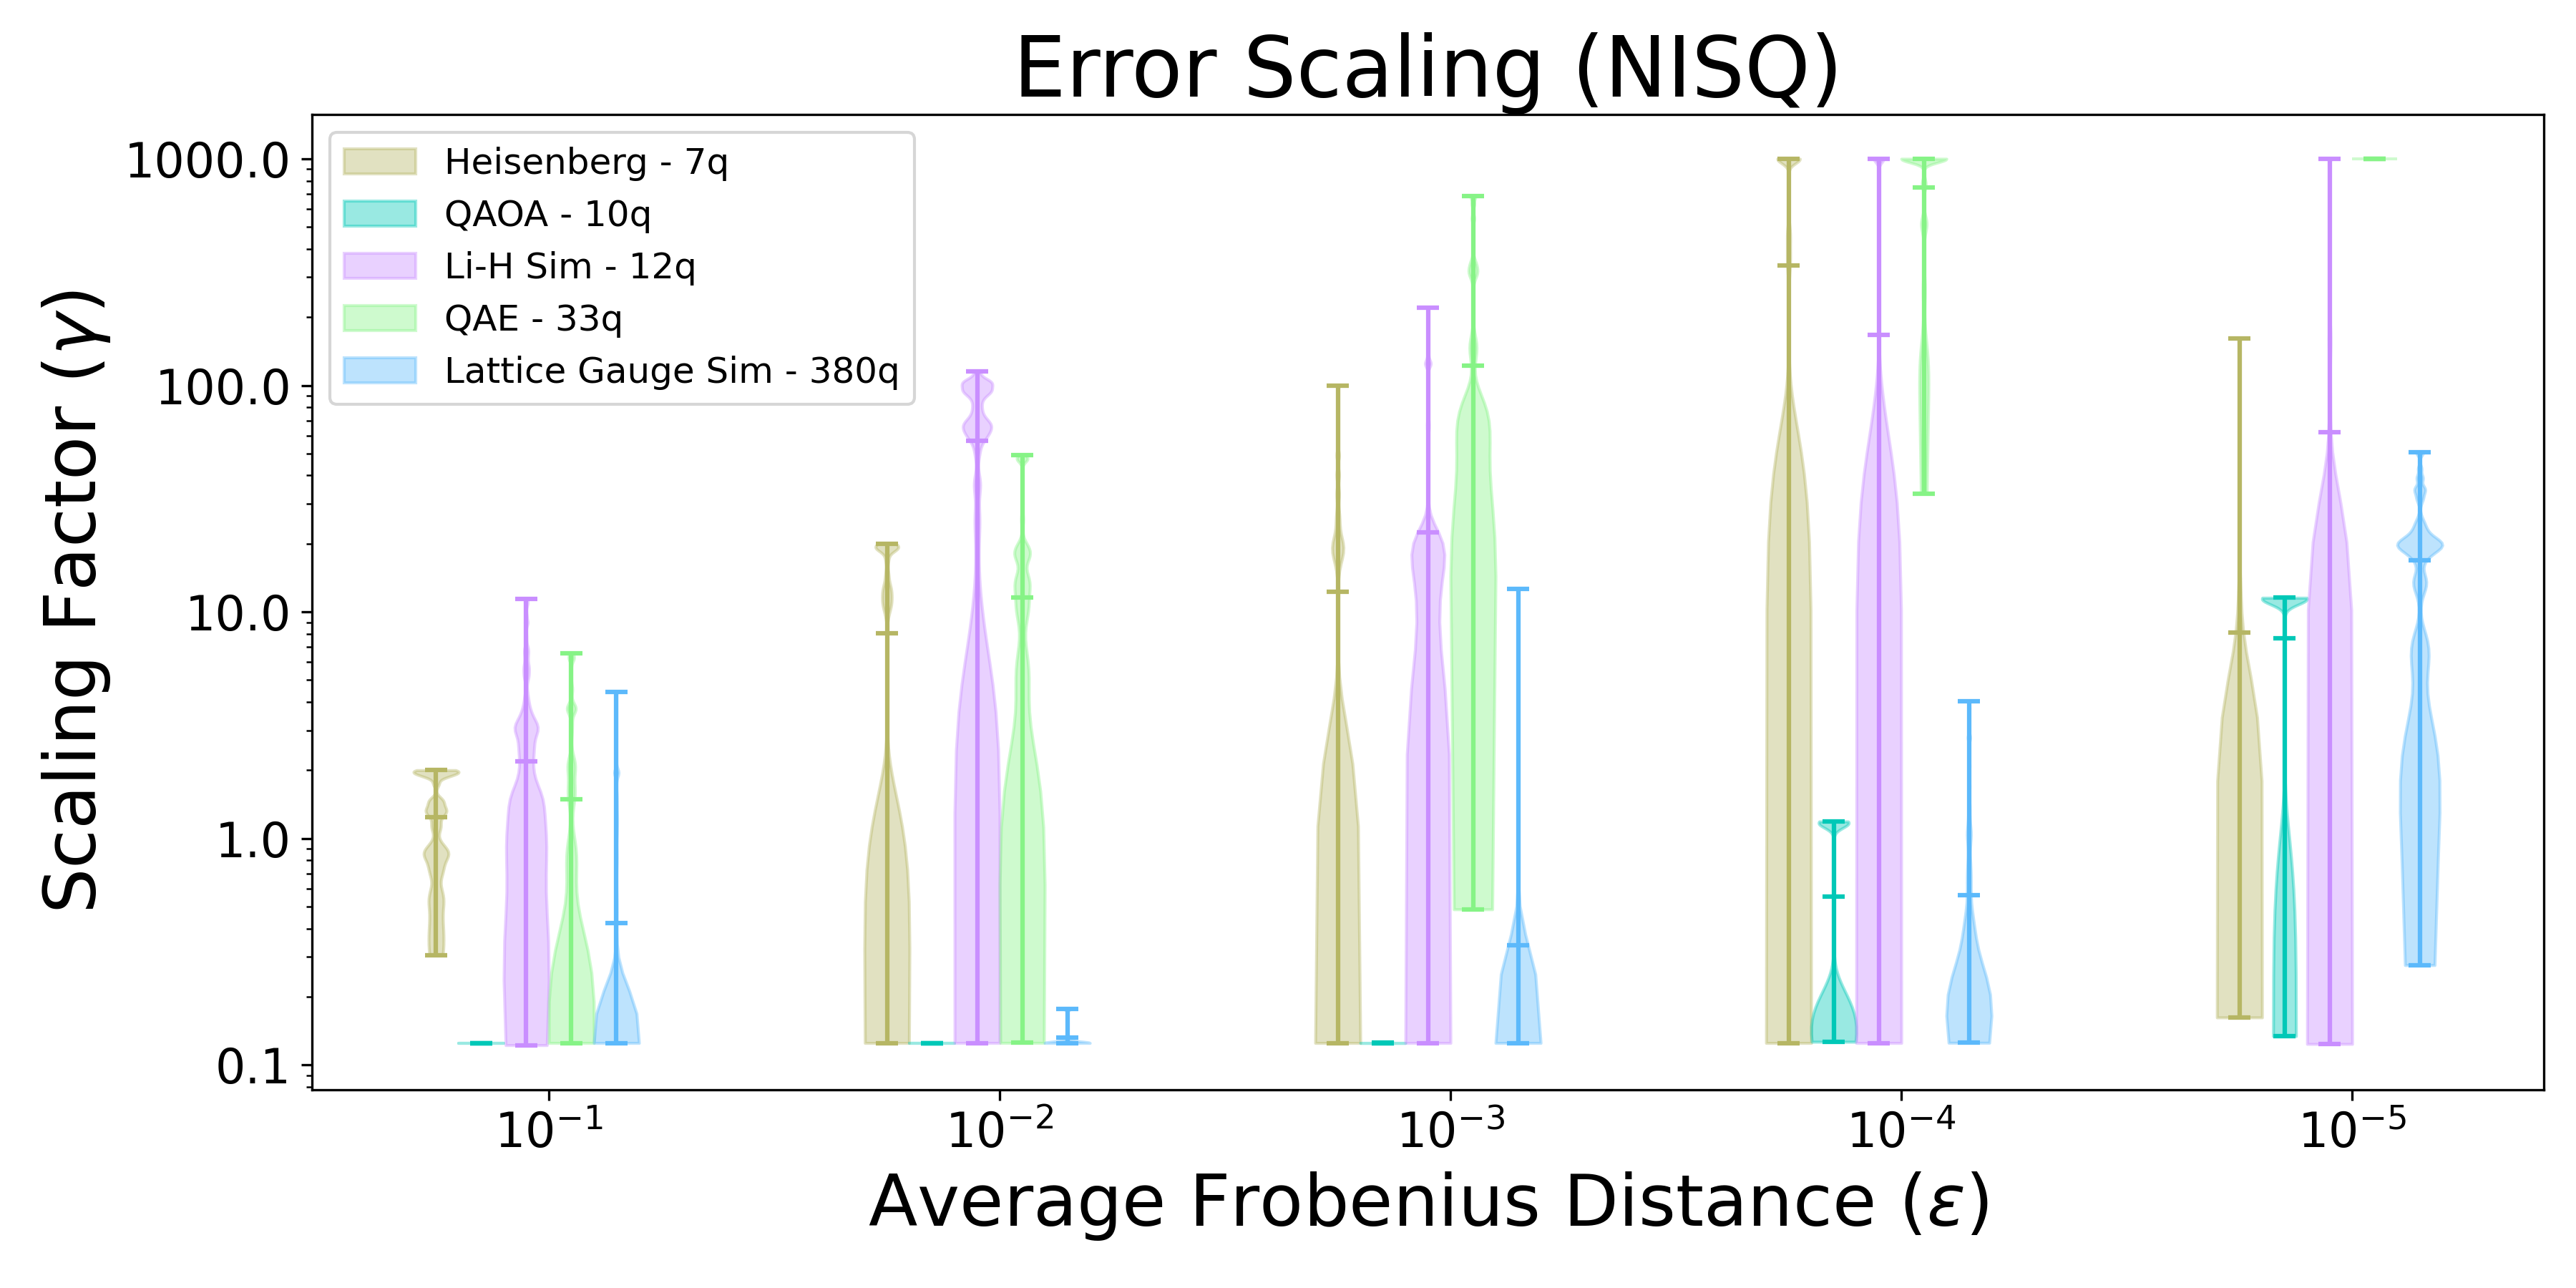
\includegraphics[width=\linewidth]{figures/supplementary/Error_scaling_final_nisq_20.png}
    \end{subfigure} \\
    \begin{subfigure}{0.7\textwidth}
        \centering
        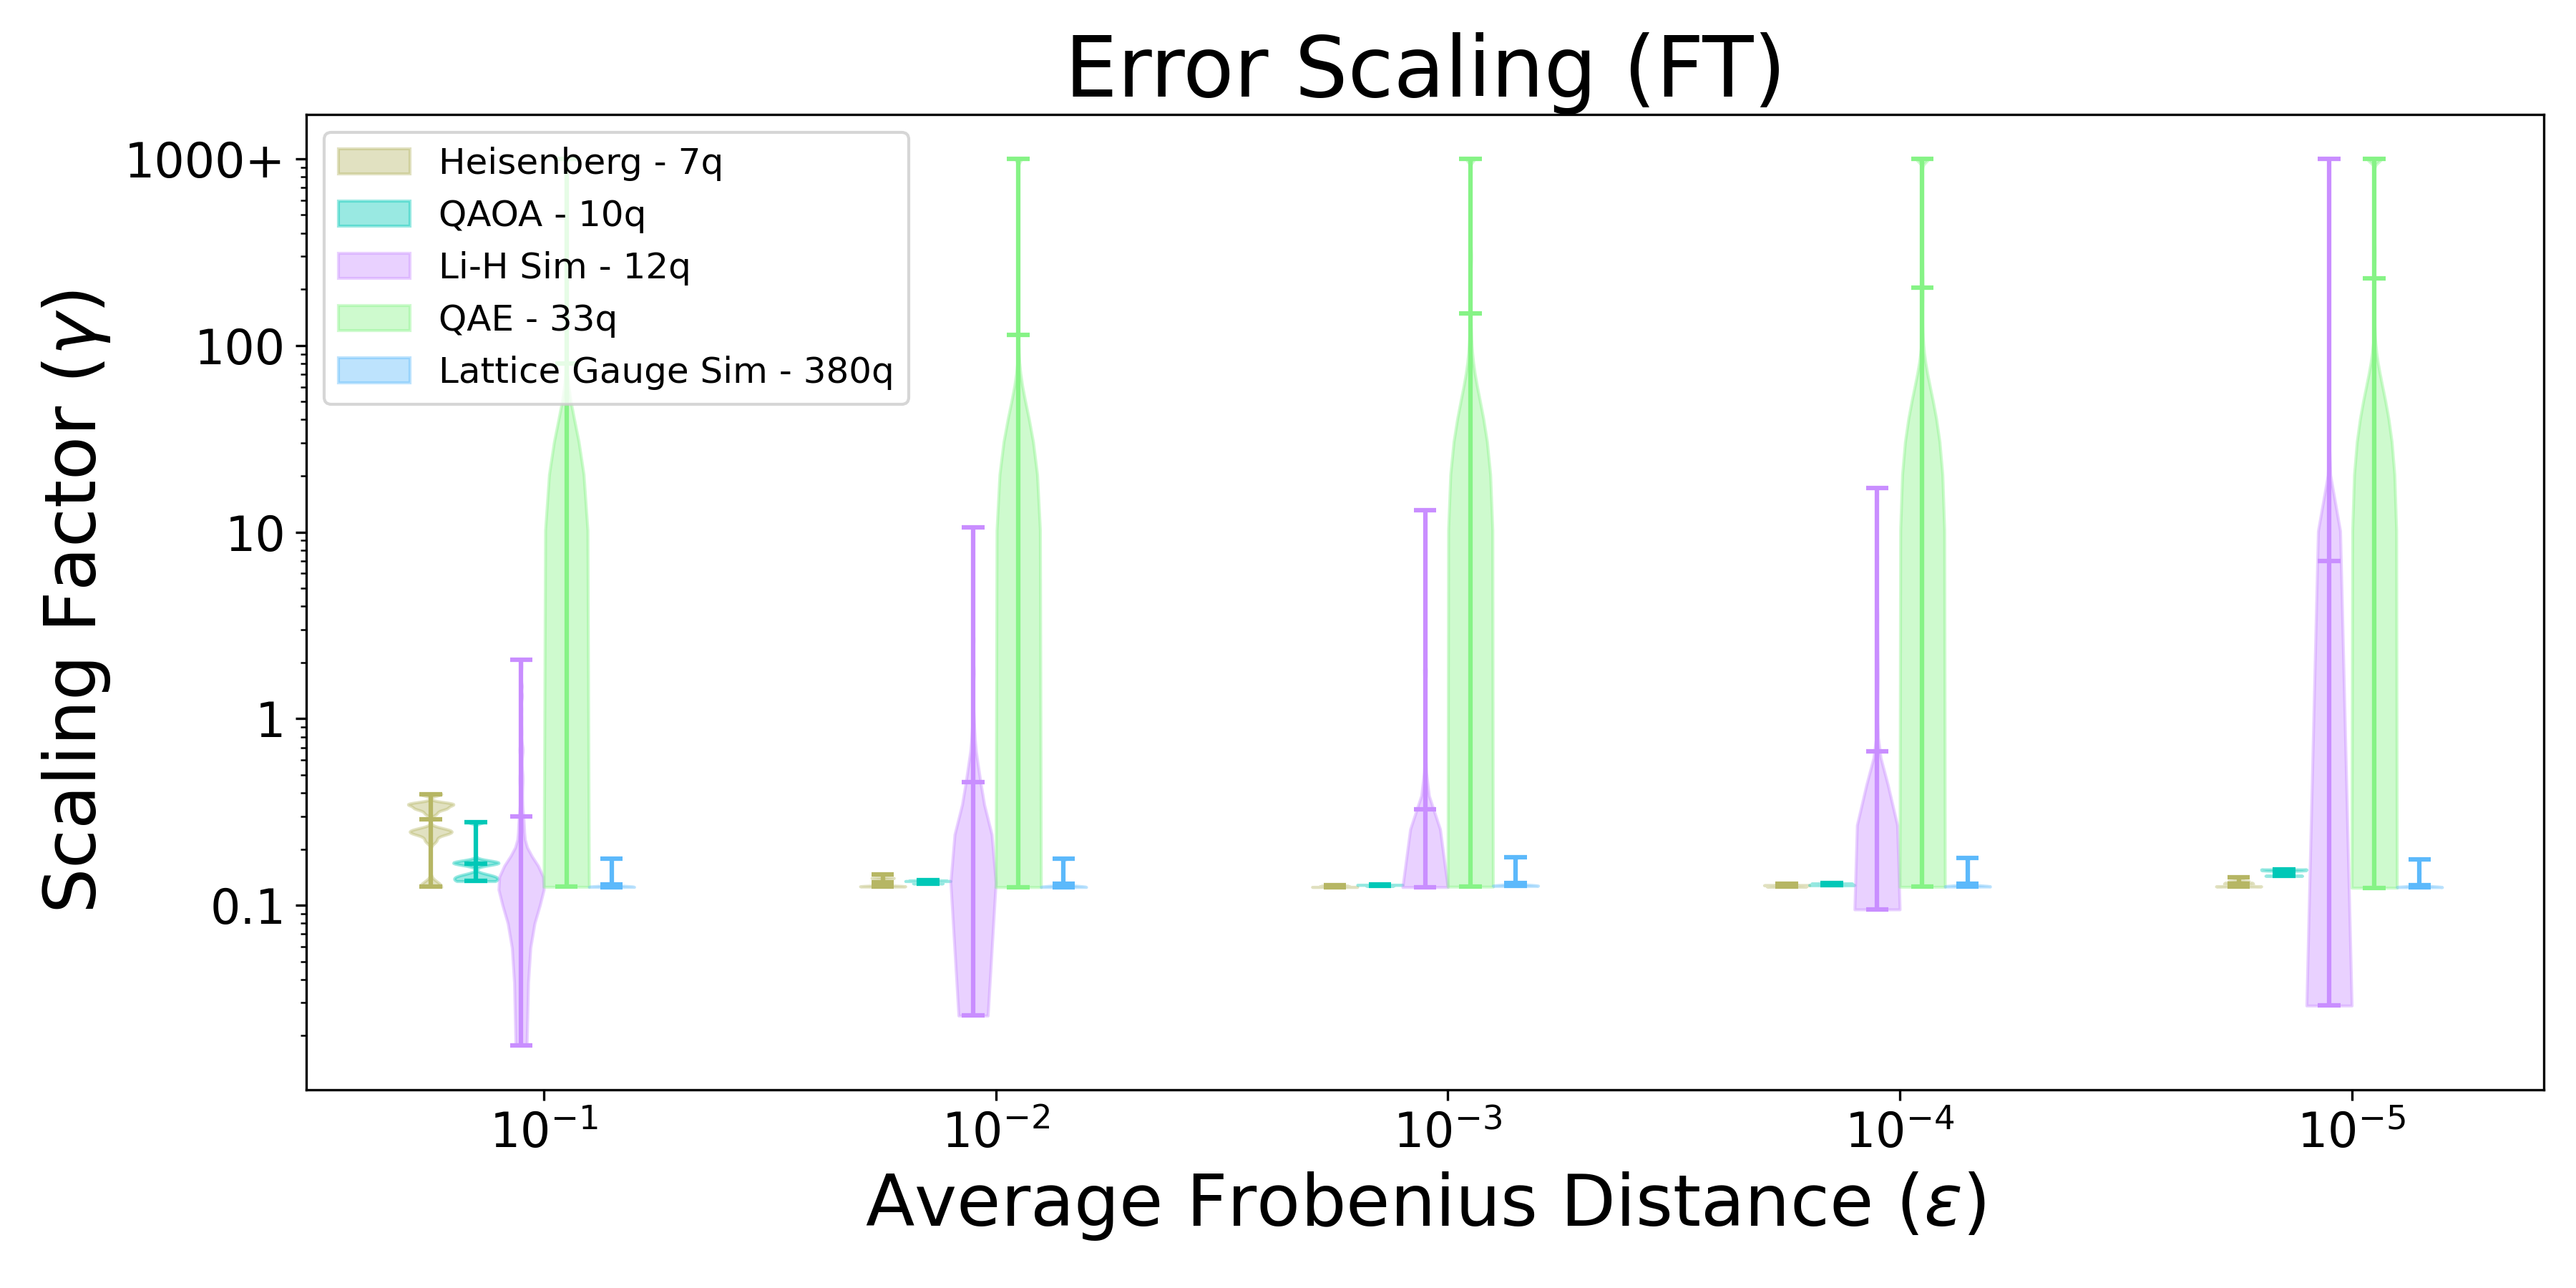
\includegraphics[width=\linewidth]{figures/supplementary/Error_scaling_final_cliff_20.png}
    \end{subfigure}
    \caption{Quadratic scaling factor $\gamma$ as a function of $\epsilon$, for some of the benchmarks.  
    Top: NISQ workflow (minimizing CNOT count).  
    Bottom: FT workflow (minimizing $T$-count).}
    \label{fig:error_scaling}
\end{figure*}


\begin{figure*}[t]
    \centering
    \begin{subfigure}{0.7\textwidth}
        \centering
        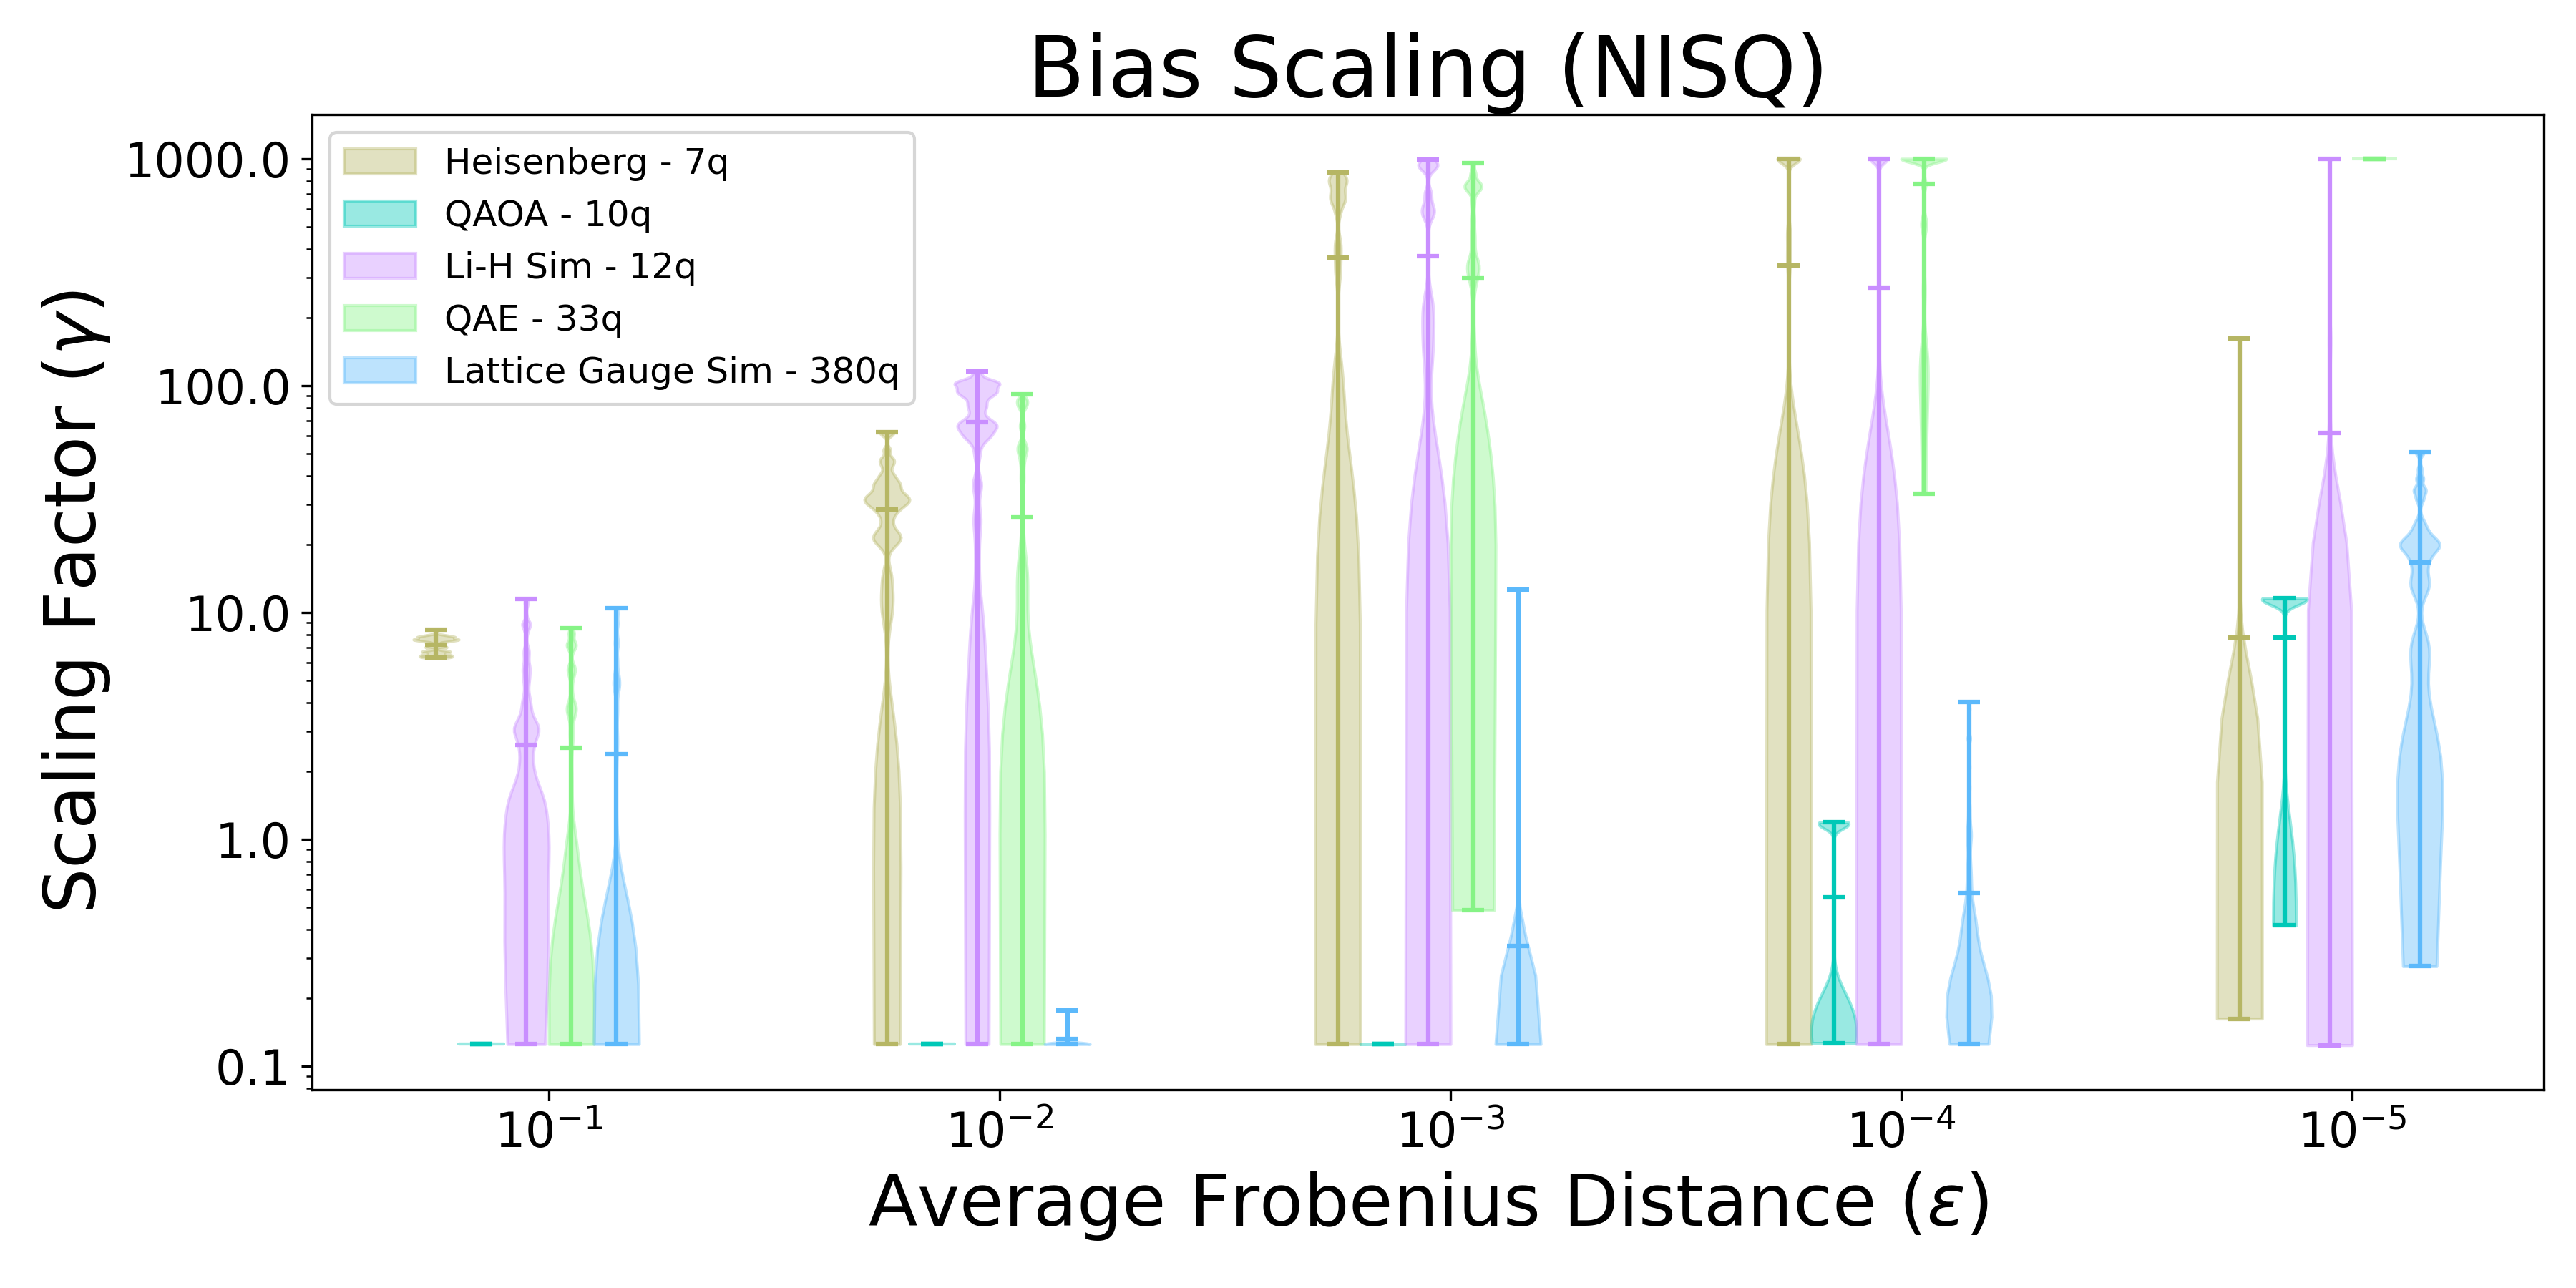
\includegraphics[width=\linewidth]{figures/supplementary/Bias_scaling_final_nisq_20.png}
    \end{subfigure} \\
    \begin{subfigure}{0.7\textwidth}
        \centering
        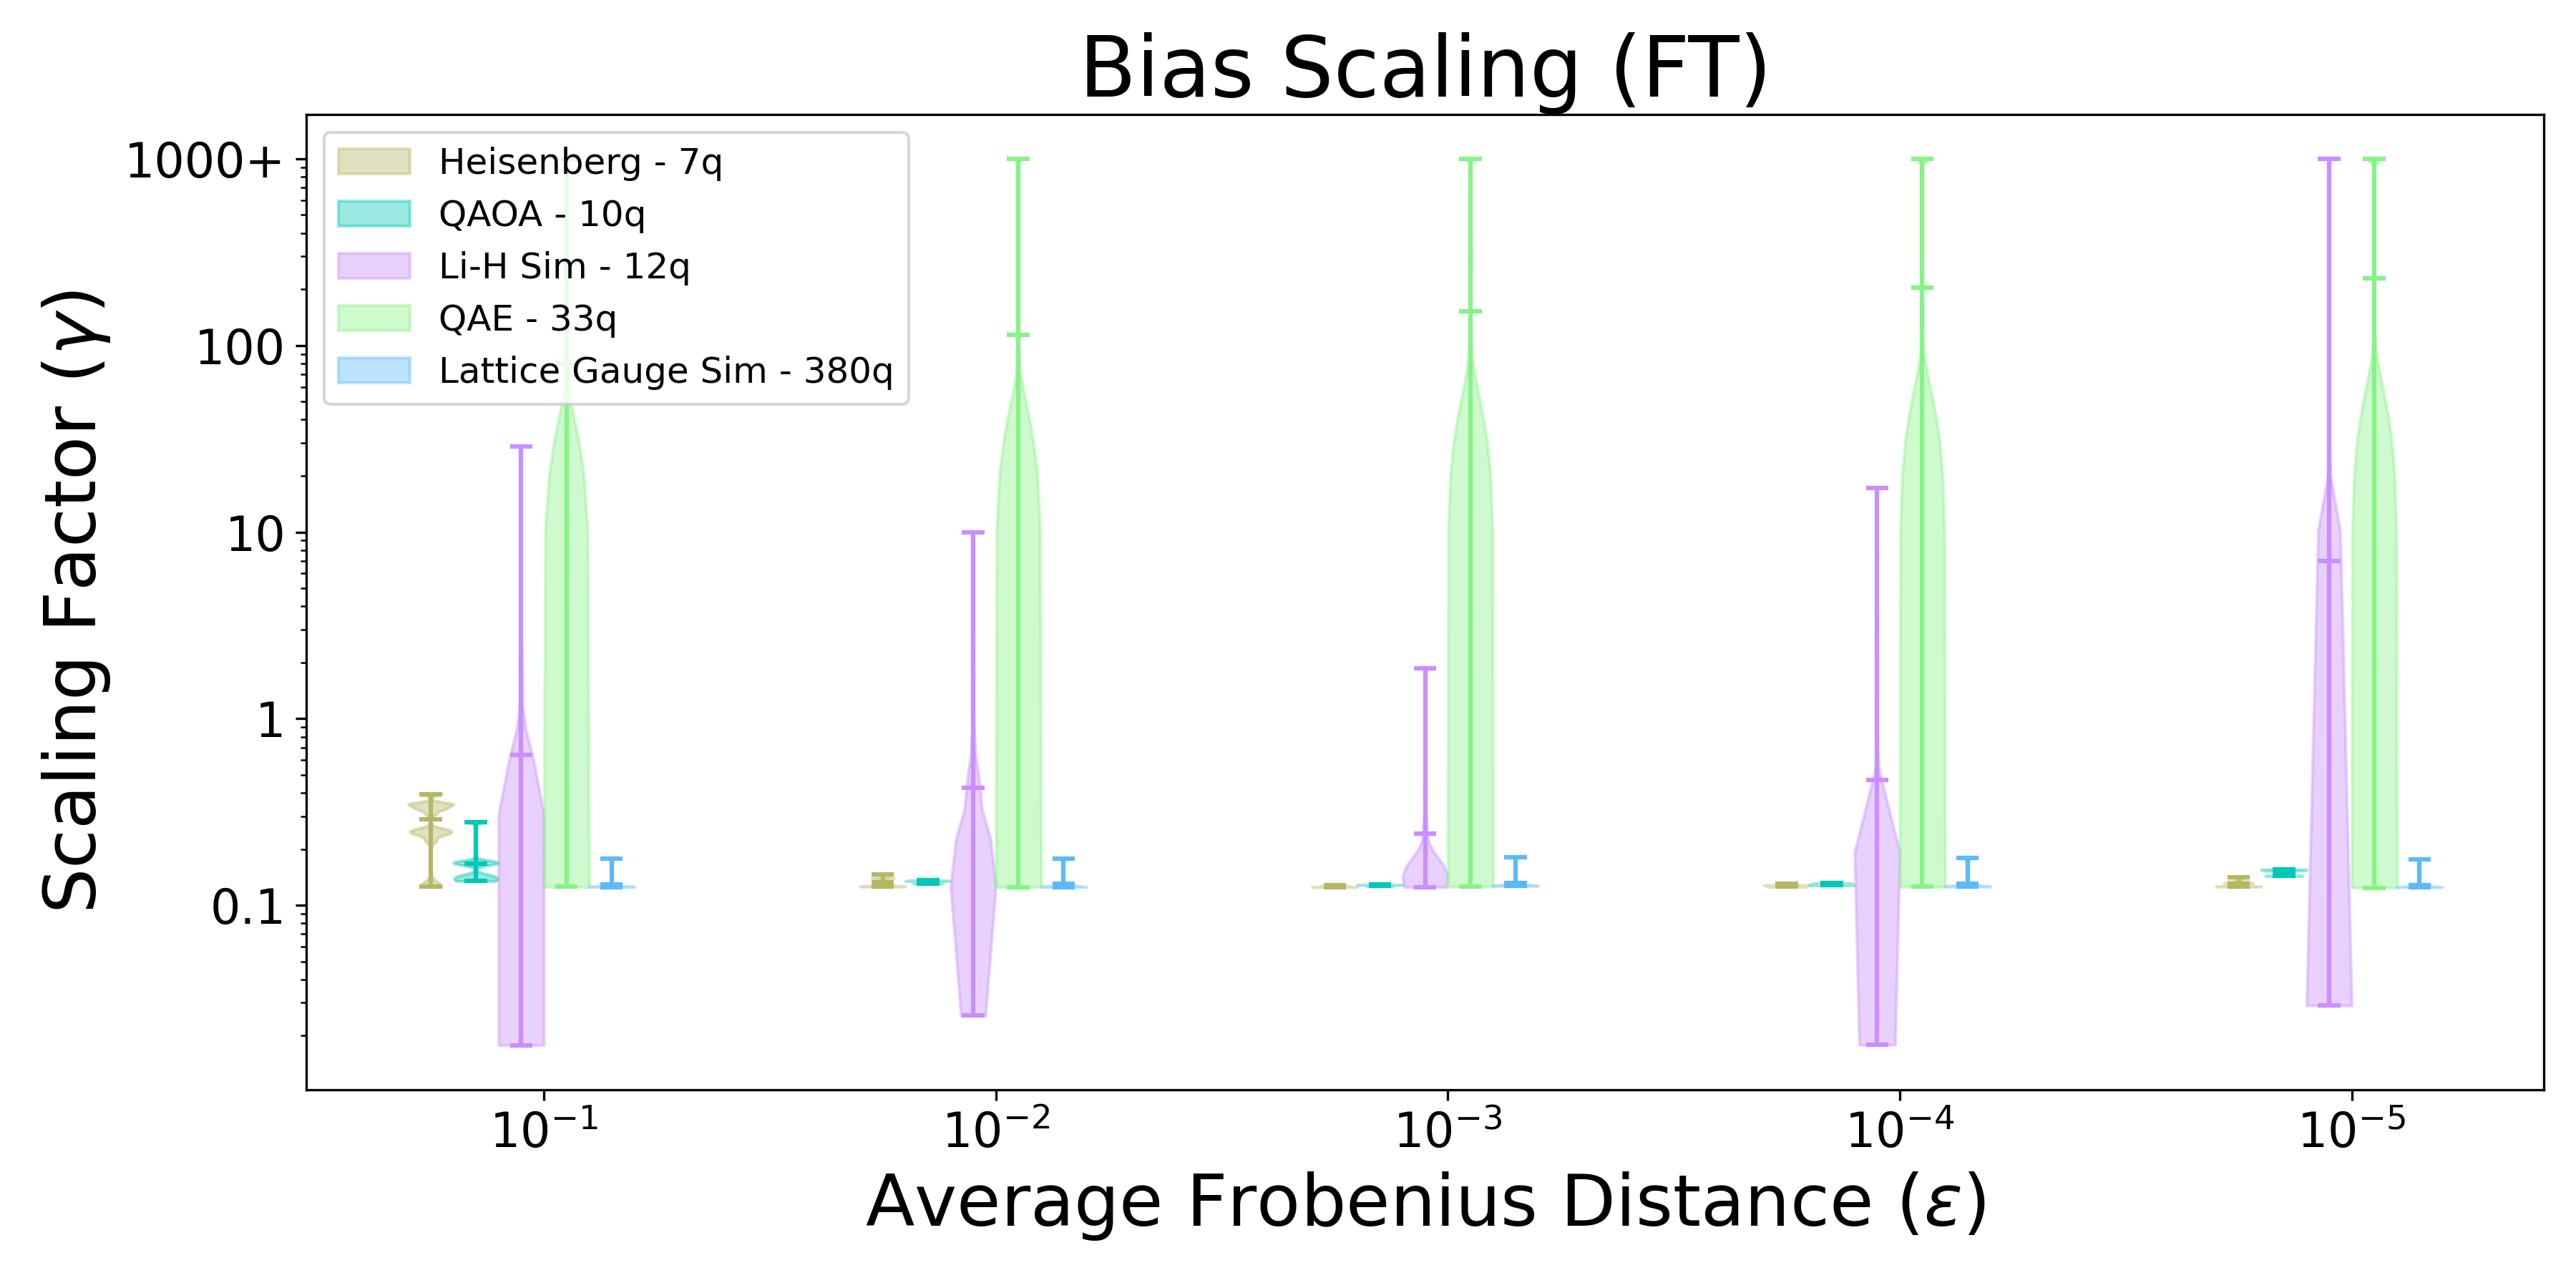
\includegraphics[width=\linewidth]{figures/supplementary/Bias_scaling_final_cliff_20.png}
    \end{subfigure}
    \caption{Quadratic scaling factor for the bias $\gamma_B$ as a function of $\epsilon$, for some of the benchmarks.  
    Top: NISQ workflow (minimizing CNOT count).  
    Bottom: FT workflow (minimizing $T$-count).}
    \label{fig:bias_scaling}
\end{figure*}

Figure \ref{fig:error_scaling} shows violin plots of the \emph{quadratic scaling factor} (QCF),  
\[
\gamma \equiv \frac{\normf{\sum_{i=1}^{M^\k} p^\k_i U^\k_i - V^\k}}{\epsilon^2},
\]  
for all blocks across many of our benchmarks.  
We expect $\gamma = O(1)$ when quadratic reduction of error is achieved.  
The plots indicate that, for most $\epsilon$ values, a significant subset of blocks in both NISQ and FT workflows achieve $O(\epsilon^2)$ scaling. In particular, almost all of the blocks in the FT workflow achieve $O(\epsilon^2)$ scaling. This is because we include a secondary compilation workflow, which trades off numerical synthesis resource reduction for improved scaling.

Our workflow does not require all blocks to satisfy Eq. \eqref{eq:wee_cond}. Blocks that fail to meet the condition are left unmodified, preserving the original circuit for those segments.  
This selective replacement explains why some benchmarks exhibit no gate count reduction (Tables 1 and 2 in the main text, particularly in the NISQ setting at small $\epsilon$). 

We also derived a sufficient condition for satisfying the ReWEE condition in terms of the bias of the compiler output,
\begin{align}
    \normf{\E{U} - V} < O(\epsilon^2).
\end{align}
We can define a quadratic scaling factor for the bias also, $\gamma_B \equiv \normf{\E{U}-V}/\epsilon^2$, and this quantity is displayed in Figure \ref{fig:bias_scaling} for all blocks of many of our benchmarks.


\section{Theoretical proofs}
In this section we provide proofs of Lemma 2 and Lemma 3 in the Methods section of the main text. Before restating the Lemmas and providing proofs, we recall several definitions from the main text.

$V$ is a target unitary on $n$ qubits, and $U_i$ are a set of approximate compilations of $V$ provided by a compiler. The compilation workflow can have probabilistic elements, and therefore we think of $U_i$ as independent, identically distributed (\emph{i.i.d.}) samples from some distribution of approximate compilations. The statistical properties we will demand of the compilation workflow are:
\begin{enumerate}
\item The compilations should all be close to the ideal, in the sense,
    \begin{align}
	\normf{U_i-V} \leq \epsilon, \quad \forall i		
		\label{eq:ass1}
	\end{align}
	\item The compilations have bounded variance, in the sense, $\E{U_i} \equiv \E{U}$ is independent of $i$, and
	\begin{align}
		\E{\normf{U_i - \E{U}}^2} \leq \epsilon', \quad \forall i
		\label{eq:ass2}
	\end{align}
\end{enumerate}
The expectations in these expressions and in the rest of this note are over the distribution of compilations generated by the compiler that satisfy Condition 1, \ie
$ \E{f(U)} = \int {\rm d}\mu_V(U) f(U), $
where ${\rm d}\mu_V(U)$ is the measure over $SU(2^n)$ defined by the compiler output that satisfies Condition 1 when the target is $V$ (the expectation symbol $\E{}$ should have a subscript $V$ but we omit this for ease). In addition,
\begin{enumerate}
    \item Define the channels $\mathcal{V}[\rho] = V \rho V\dg$, $\mathcal{U}_i[\rho] = U_i \rho U_i\dg$, and $\mathcal{U}[\rho] = \sum_i p_i U_i \rho U_i\dg$, for some probabilities $\{p_i\}$.
    \item $J_{\mathcal{E}} \equiv \sum_{i,j=1}^d \mathcal{E}(\ket{i}\bra{j})\otimes \ket{i}\bra{j}$ is the Choi matrix representation of the channel $\mathcal{E}$, which we assume to be acting acting on $d\times d$ density matrices and outputting density matrices of the same size.
\end{enumerate}

\noindent \emph{\bf Lemma 2:} \emph{Let $V$ and $U_i$ be defined as above. Given probabilities $\{p_i\}_{i=1}^M$, ($\sum_{i=1}^M p_i=1$), a sufficient condition for achieving $\E{\normf{\sum_{i=1}^M p_i U_i - V}} \leq O(\epsilon^2)$ is the \emph{reduced bias condition}: $\normf{\E{U}-V} \leq O(\epsilon^2)$.}

\noindent \textit{Proof:} First, note that $\E{\normf{\sum_{i=1}^M p_i U_i - V}} \leq O(\epsilon^2)$ follows directly from $\E{\normf{\sum_{i=1}^M p_i U_i - V}^2} \leq O(\epsilon^4)$ through an application of Jensen's inequality, and so we prove the latter statement.
\begin{align}
    \E{\normf{\sum_{i=1}^M p_i U_i - V}^2} & \leq \E{\normf{\frac{1}{M}\sum_{i=1}^M U_i - V}^2} 
	   = \normf{\overline{bias}}^2 + \frac{1}{M}\overline{var} + \left(1-\frac{1}{M}\right)\overline{covar}, 
       \label{eq:b-v-c} 
\end{align}
where,
\begin{align}
	\overline{bias} &= (\E{U} - V) \label{eq:bias} \\
	\overline{var} &= \frac{1}{M}\sum_{i=1}^{M} \E{\normf{U_i - \E{U}}^2} \label{eq:var} \\
	\overline{covar} &= \frac{1}{M(M-1)}\sum_{i=1}^M \sum_{j \neq i}^M \mathbb{E} \left\{ \tr[(U_i-\E{U})\dg \cdot (U_j - \E{U})] \right\} 
    \label{eq:covar}
\end{align}
The first inequality follows from the fact that the weights $p_i$ are optimized to reduce the ensemble error. The equality on the second line follows from using the definition of the Frobenius norm to decompose the quantity of interest in a \emph{bias-variance-covariance} decomposition, a well-known decomposition of generalization error of ensembles of estimators in machine learning \cite{Ueda_1996, Brown_20005}. Here, $\overline{bias}$ is the bias of the (uniform) ensemble, $\overline{var}$ is the (sample) average of the variance of the members of the ensemble, and $\overline{covar}$ is the covariance of the ensemble members. Since the ensemble members are sampled \emph{i.i.d.} from the compiler output distribution, the covariance term is zero. In addition, using the fact that the samples have bounded variance, Eq. \eqref{eq:ass2}, we get
$\E{\normf{\sum_{i=1}^M p_i U_i - V}^2} \leq \normf{\E{U}-V}^2 + \frac{\epsilon'}{M}$.
This quantity can be bounded as $O(\epsilon^4)$ by satisfying the reduced bias condition and choosing $M \geq \epsilon'/\epsilon^4$. \QED
\\

\noindent \emph{\bf Lemma 3:} \emph{Let $V$ and $U_i$ be defined as above, and let these unitaries act on a register of $n$ qubits; \ie ${\rm dim}~ V = {\rm dim}~ U_i = 2^n \equiv d$. Define $\mathcal{V}[\rho] = V \rho V^{\dagger}$ as a target channel, and $\mathcal{U}[\rho] = \sum_{i=1}^M p_i U_i \rho U_i\dg$ as an optimized ensemble channel, such that $d_\diamond(\mathcal{V}, \mathcal{U})\leq O(\epsilon^2)$. Further, let $\hat{\mathcal{U}}[\rho] = \frac{1}{T}\sum_{i=1}^T U_{\sigma(i)} \rho U_{\sigma(i)}\dg$ be the empirical channel defined by sampling and averaging over $U_i$ according to the distribution $\{p_i\}$ -- \ie $\sigma(i) \in \{1,...,M\}$. For $\epsilon, \delta \in (0,1)$, $\pr\left\{ d_\diamond(\mathcal{V}, \hat{\mathcal{U}}_T) \leq O(\epsilon^2) \right\} > 1-\delta$, given
\begin{align}
    T \geq \frac{2v + \frac{2}{3}R \left(\epsilon^2/(2d^2)\right) }{\left(\epsilon^2/(2d^2)\right)^2}\log \frac{2d^2}{\delta}
    \label{eq:T_bound}
\end{align}
Here, $v \equiv \normo{\sum_{i=1}^M p_i (J_i - J_{\mathcal{U}})^2}, R \equiv \max_i \normo{J_i - J_{\mathcal{U}}}$, and $J_i (and J_{\mathcal{U}}$) are the $d^2$-dimensional Choi matrices associated to the channel $\mathcal{U}_i[\rho] = U_i \rho U_i^{\dagger}$ (and $\mathcal{U}$).}

\noindent \textit{Proof:} We begin by an application of the triangle inequality:
\begin{align}
    d_\diamond(\mathcal{V}, \hat{\mathcal{U}}) &\leq  d_\diamond(\mathcal{V}, \mathcal{U}) +  d_\diamond(\mathcal{U}, \hat{\mathcal{U}}) \nn \\  
    & = O(\epsilon^2) + d_\diamond(\mathcal{U}, \hat{\mathcal{U}}),
    \label{eq:lemma3_1}
\end{align}
and hence we are left with the task of determining the sample size $T$ necessary to satisfy $d_\diamond(\mathcal{U}, \hat{\mathcal{U}}) \leq \epsilon^2$. Therefore, 
\begin{align}
    d_\diamond(\mathcal{U}, \hat{\mathcal{U}}) &\equiv \normd{\mathcal{U}- \hat{\mathcal{U}}} \nn \\
    & \leq \normt{J_\mathcal{U} - J_{\hat{\mathcal{U}}}} \nn \\
    & \leq 2d^2 \normo{J_\mathcal{U} - J_{\hat{\mathcal{U}}}},
\end{align}
where the first inequality follows from an identity established by Watrous \cite[Exercise 3.6]{watrous_2018}, the second is the application of a standard norm inequality ($\normt{A}\leq {\rm rank}(A)\normo{A}$), and an overestimate of the relevant rank: ${\rm rank}(J_\mathcal{U} - J_{\hat{\mathcal{U}}}) \leq {\rm rank}(J_\mathcal{U} ) + {\rm rank}(J_{\hat{\mathcal{U}}}) \leq 2d^2$. In the above, the Choi matrices are explicitly, $J_\mathcal{U} = \sum_{i=1}^M p_i J_i$ and $J_{\hat{\mathcal{U}}} = \frac{1}{T} \sum_{i=1}^T J_i$, with $J_i \equiv J_{\mathcal{U}_i}$. 

Now that the error is expressed in terms of an operator norm, we can apply standard Bernstein matrix concentration inequality \cite{tropp_2015} to get, 
\begin{align}
    \pr\left\{ d_\diamond(\mathcal{U}, \hat{\mathcal{U}}) \geq \epsilon^2 \right\} \leq \pr\left\{ \normo{J_\mathcal{U} - J_{\hat{\mathcal{U}}}} \geq \frac{\epsilon^2}{2d^2} \right\} \leq 2d^2 \exp\left(-\frac{T(\frac{\epsilon^2}{2d^2})^2}{2v + \frac{2}{3}R \frac{\epsilon^2}{2d^2}}\right),
\end{align} 
where $v$ and $R$ are the variance and maximum deviation as defined in the Lemma statement. In order for the right-hand side to be at most $\delta$, the sample size given in Eq. \eqref{eq:T_bound} is sufficient. Finally, combining this with the statement in Eq. \eqref{eq:lemma3_1} yields the Lemma statement. 
\QED

\subsection{Statistics of factors entering sample complexity}
While the formal sample complexity bound in Lemma 3 scales with $\epsilon$ as $O(1/\epsilon^4)$, in the main text we claimed that in practice, $v=O(\epsilon^2)$, and therefore, the number of samples needed is $O(1/\epsilon^2)$. Figure 5 in the main text provided evidence for this gentler scaling for one of the benchmarks in our study. While Lemma 3 is stated in terms of diamond distance between the empirical channel and the ensemble channel, this error is infeasible to evaluate numerically because of the difficulty of calculating the diamond distance for channels acting on many qubits. Therefore, in Figure 5 of the main text, we showed the trace distance error in the output, $\normt{\rho_{T} - \rho_i}$,
where $\rho = \sum_{i=1}^M p_i U_i \rho_{0} U_i\dg$ is the output of the ensemble channel for random input state $\rho_{0}$, and $\rho_{T} = \frac{1}{T}\sum_{i=1}^T U_i \rho_{0} U_i\dg$ is the output of the empirical channel for the same input (the $U_i$ in the empirical channel are sampled according to the distribution $\{p_i\}$ set by the ensemble channel). 

The equivalent sample complexity bound for this error metric is $\pr\{\normt{\rho_{T} - \rho} \geq \epsilon^2\} \leq 1-\delta$, if
\begin{align}
    T \geq \frac{2v + \frac{2}{3}R \left(\epsilon^2/(2d)\right) }{\left(\epsilon^2/(2d)\right)^2}\log \frac{2d}{\delta},
    \label{eq:T_bound_state} 
\end{align}
where $v \equiv \normo{\sum_{i=1}^M p_i (\rho_i - \rho)^2}, R \equiv \max_i \normo{\rho_i - \rho}$, and $\rho_i = U_i\rho_0 U_i\dg$. Calculating the values $v$ and $R$ is difficult for most of the benchmarks we studied, even in this case, because $M$ can be very large for full circuits, and thus computing the ideal ensemble output $\rho$ is numerically intensive. Instead, we compute these variance and maximum deviation values, $v$ and $R$, for all blocks in two of our benchmark circuit ensembles. As shown in Fig. \ref{fig:vR}, $v \ll \epsilon^2$ in practice, which explains the gentler scaling of $T$ required to approximate the ensemble channel with the empirical channel.

\begin{figure*}[ht]
    \centering
        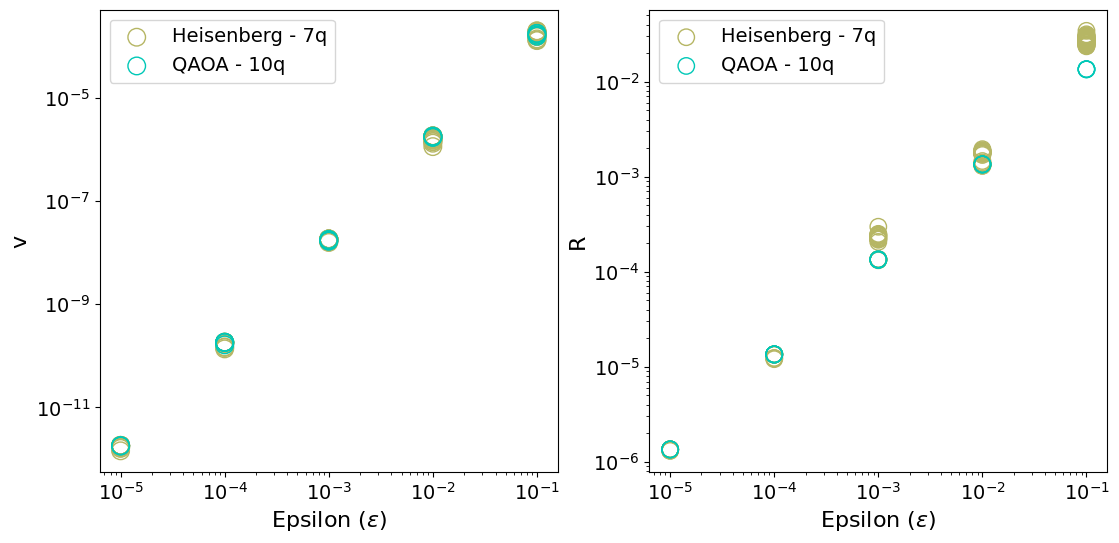
\includegraphics[width=0.7\linewidth]{figures/supplementary/v_R_all_circs_1_final.png}
    \caption{Values of variance and maximum deviation factors, $v$ and $R$, entering the sample complexity bound Eq. \eqref{eq:T_bound_state} for each block of two benchmark circuits.}
    \label{fig:vR}
\end{figure*}

\newpage

\documentclass[fleqn,10pt]{wlscirep}
\usepackage[utf8]{inputenc}
\usepackage[T1]{fontenc}
\usepackage{wrapfig}
\usepackage{subcaption}
\usepackage{multirow}
\usepackage{multicol}
\usepackage{tikz}
\usepackage{graphicx}
\usepackage{standalone}

\newcommand{\eg}{\emph{e.g.,~}}
\newcommand{\ie}{\emph{i.e.,~}}
\newcommand{\bx}{\mathbf{x}}
\newcommand{\by}{\mathbf{y}}
\newcommand{\bp}{\mathbf{p}}
\newcommand{\hx}{\hat{x}}
\newcommand{\hp}{\hat{p}}
\newcommand{\ket}[1]{\vert#1\rangle}
\newcommand{\bra}[1]{\langle #1\vert}
\newcommand{\expect}[1]{\langle #1\rangle}
\newcommand{\dg}{^\dagger}
\newcommand{\nn}{\nonumber}
\newcommand{\pr}{{\rm Pr}}

\newcommand{\normf}[1]{\left\lVert #1 \right\rVert_F}
\newcommand{\normo}[1]{\left\lVert #1 \right\rVert}
\newcommand{\normt}[1]{\left\lVert #1 \right\rVert_1}
\newcommand{\normd}[1]{\left\lVert #1 \right\rVert_\diamond}
\newcommand{\E}[1]{\mathbb{E}\left\{ #1 \right\}}

\newcommand{\tr}{{\rm tr}}
\renewcommand{\k}{{(k)}}
\newcommand{\p}{{\bf\sf p}}
\newcommand{\braket}[2]{\langle #1 \vert #2 \rangle}

\newcommand*{\QED}{\null\nobreak\hfill\ensuremath{\blacksquare}}%

\makeatletter
\renewcommand{\@maketitle}{%
{%
\thispagestyle{empty}%
\vskip-36pt%
{\raggedright\sffamily\bfseries\fontsize{20}{25}\selectfont \@title\par}%
\vskip10pt
{\raggedright\sffamily\fontsize{12}{16}\selectfont  \@author\par}
\vskip25pt%
}%
}%
\makeatother

\newcommand{\red}[1]{{\color{red}#1}} 
\newcommand{\needcite}{{\color{red}[XX]~}}
\long\def\comment#1{}
\long\def\note#1{{\em #1 }}
\def\parah#1{\vspace*{0.0in} \noindent{\bf #1:}}

\title{Supplementary Information for: Application Scale Quantum Circuit Compilation with Controlled Error}

\author[1,2,*]{Justin Kalloor}
\author[3]{Lucas Kovalsky}
\author[1,2]{Mathias Weiden}
\author[2]{John Kubiatowicz}
\author[1]{Ed Younis}
\author[1]{Costin Iancu}
\author[3,+]{Mohan Sarovar}
\affil[1]{Computational Research Division, Lawrence Berkeley National Laboratory, Berkeley, CA, 94702, USA}
\affil[2]{Department of Electrical Engineering and Computer Science, University of California, Berkeley, CA, 94702, USA}
\affil[3]{Quantum Algorithms and Applications Collaboratory, Sandia National Laboratories, Livermore, CA, 94550, USA}

\affil[*]{jkalloor3@berkeley.edu}
\affil[+]{mnsarov@sandia.gov}



\begin{document}

\flushbottom
\maketitle

\section{Description of benchmark applications and circuits}
For our benchmarks, we use a variety of quantum algorithms across different domains of interest.

\subsection*{Hamiltonian Simulation Algorithms}
\begin{enumerate}
    \item \textbf{SU(2) Lattice Gague Simulation} - We follow the construction outlined in the paper by Rahman et. al \cite{rahman_2022} to simulate the motion of an excitation on a spatial lattice.
    \item \textbf{Li-H Molecule} - We simulate the electronic energy of a Lithium Hydride molecule. The circuit was generated using the Qiskit Nature and PySCF\cite{qiskit} libraries. The fermionic operator was mapped to qubits using a Jordan Wigner mapper\cite{jordan_wigner}. When calculating the observable, we use the Hartree Fock \cite{hartree_fock} state as the initial state.
    \item \textbf{Fermi-Hubbard Model} We run the Fermi-Hubbard model on a square lattice with periodic boundary conditions. The lattice has uniform interaction energies as well as a uniform onsite potential and was mapped to a quantum circuit with a Jordan Wigner mapper. For the observable calculations, we pass in the ground state of the non-interacting model as the initial state.
    \item \textbf{Heisenberg Model} - We simulate the nearest neighbor Heisenberg model with the Hamiltonian defined as:
    \[H = J \cdot \sum{X_iX_{i+1} + Y_iY_{i+1} + Z_iZ_{i+1}}\] and use the all zero state as the initial ground state.
\end{enumerate}

\subsection*{Arithmetic Sub-Modules}

\begin{enumerate}
    \item \textbf{Multiplier} - A quantum sub-circuit to multiply two registers and store into an output register\cite{qiskit}.
    \item \textbf{Adder} - A simple implementation of a Ripple-Carry Adder to add together two quantum registers \cite{qiskit}.
    \item \textbf{QFT Adder} - An implementation of the Draper QFT Adder \cite{draper}.
\end{enumerate}

\subsection*{Quantum Sub-Routines}

\begin{enumerate}
    \item \textbf{Quantum Amplitude Estimation (QAE)} - An implementation of the quantum amplitude estimation circuit on a Bernoulli Operator with a probability of 0.5 \cite{qiskit, brassard}.
    \item \textbf{Quantum Phase Estimation (QPE)} - We estimate the phase of a randomly generated circuit. In our 14 qubit example, we generate a 7-qubit random circuit, and use 7 qubits for precision.
\end{enumerate}

\subsection*{Quantum Optimization}

\begin{enumerate}
    \item Quantum Approximate Optimization Algorithm - An implementation of the optimization circuit given in QASMBench\cite{qasm_bench}.
\end{enumerate}

\section{``Rigid" Circuit Blocks}
\label{sec:rigid_blocks}
As ensemble generation time grows exponentially with the number of qubits, circuit partitioning allows us to scale our workflow to application-width circuits. We first split our circuit into blocks of width $w$, and then generate a block-level ensemble for each partition \emph{in parallel}. Importantly, we are able to accept/reject each ensemble based on the ReWEE condition, which gives us additional flexibility on which circuits benefit from our methodology. We do not need a perfect ensemble for the circuit as a whole; we can pick and choose which parts of the circuit benefit from approximation.

Despite this additional freedom provided by the partitioner, there are benchmarks that are unable to see any reduction in the NISQ compilation workflow. This happens when the input circuit is partitioned into ``rigid" blocks. Rigid blocks are circuits (along with their underlying unitaries) that either 1) Cannot be reduced (e.g no CNOTs can be removed without significant approximation error or 2) Only have a few approximate solutions, which are not diverse enough to form a convex hull around the original unitary.

\begin{figure}[htbp]
\centering
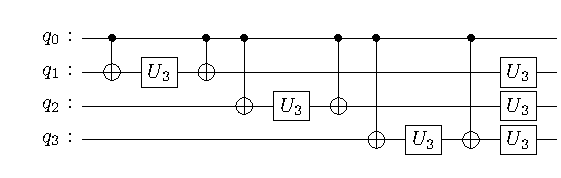
\includegraphics[width=0.55\textwidth]{figures/supplementary/rigid_block_one.pdf} \\
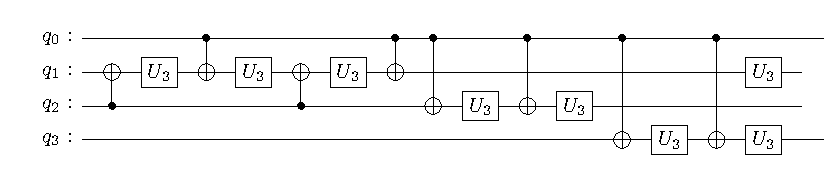
\includegraphics[width=0.8\textwidth]{figures/supplementary/rigid_block_two.pdf}
\caption{Two examples of ``rigid" circuit blocks from the QFT Adder circuit and QPE circuit.}
\label{fig:rigid_blocks}
\end{figure}

Figure \ref{fig:rigid_blocks} illustrates two examples of these rigid structures. The first block is from the QFT Adder circuit while the second block is from a QPE circuit. The first circuit contains 3 consecutive controlled rotations with the same control qubit (q0), while the second circuit contains a multi-controlled rotation and two controlled rotations. Consecutive rotations with a only a few control qubits prove difficult to reduce in the NISQ setting, since the removal of any single CNOT adds significant error to the underlying unitary. On top of that, since the control qubit is being constantly reused, it is hard to find approximate ``shortcuts" by leveraging CNOTs on surrounding qubits.

For the demonstration of our workflow shown in this work, we use a block size of $4$, while the standard BQSKit compile width is $3$. We found that by increasing the block size, both the reduction quality and probability of finding a convex hull improved, as the partitions were more likely to have many control and target qubits and be less rigid. We predict that increasing the block size to larger and larger sizes would continue to improve our results, albeit at the cost of compilation time.




\section{Statistics of ensemble error reduction}
\label{sec:error_scaling}

The benefits of using an ensemble channel are guaranteed only if the ReWEE condition is satisfied, \ie the weighted ensemble error is quadratically reduced, 
\begin{align}
    \normf{\sum_{i=1}^{M^\k} p^\k_i U^\k_i - V^\k} \leq O(\epsilon^2), 
\label{eq:wee_cond}
\end{align}
when each compilation, $U^\k_i$, is performed to error $\epsilon$.  
In practice, it is challenging to construct an ensemble of approximate circuits that both:  
\begin{enumerate}
    \item Uses fewer resource-intensive gates (e.g., CNOT or $T$ gates) on average than the original circuit, and  
    \item Satisfies Eq. \eqref{eq:wee_cond}.  
\end{enumerate}  
While explicit algorithms exist for guaranteeing Eq. \eqref{eq:wee_cond} \cite{PhysRevA.95.042306}, they are difficult to scale to multi-qubit circuits and do not provide resource efficiency guarantees.

In the main text we have shown that both criteria can be met for several of the benchmarks we studied.   
Here, we present statistics that explain how this is achieved through quadratic reduction in the weighted ensemble error and selective filtering of circuit blocks.



\begin{figure*}[t]
    \centering
    \begin{subfigure}{0.7\textwidth}
        \centering
        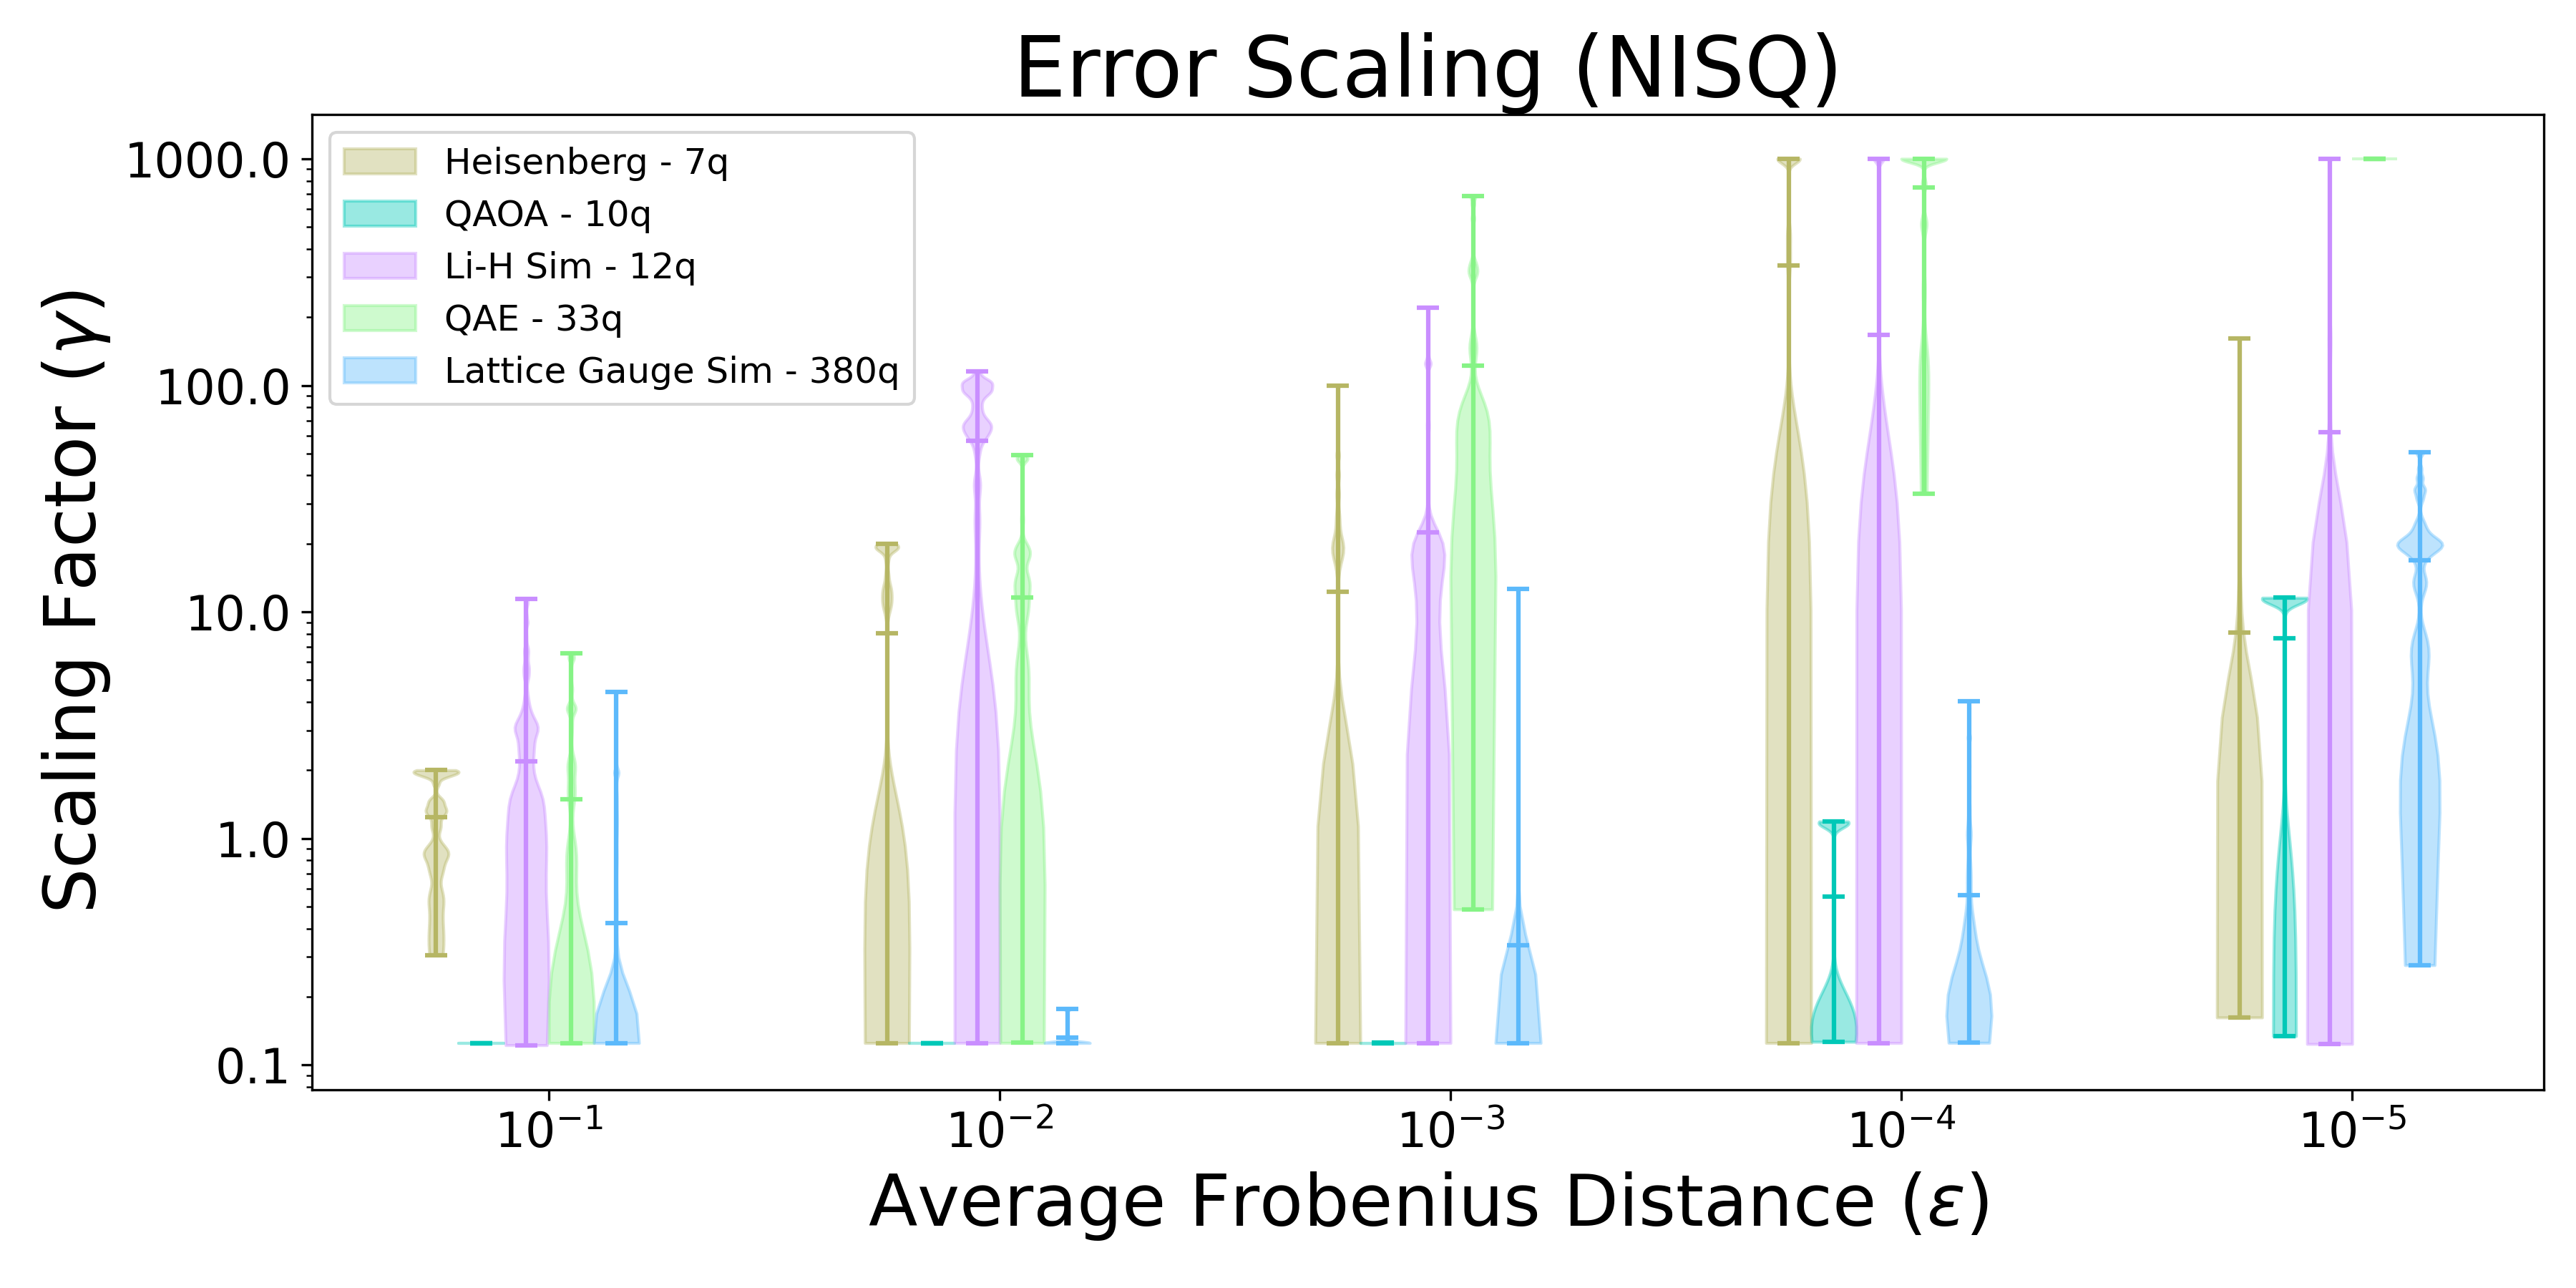
\includegraphics[width=\linewidth]{figures/supplementary/Error_scaling_final_nisq_20.png}
    \end{subfigure} \\
    \begin{subfigure}{0.7\textwidth}
        \centering
        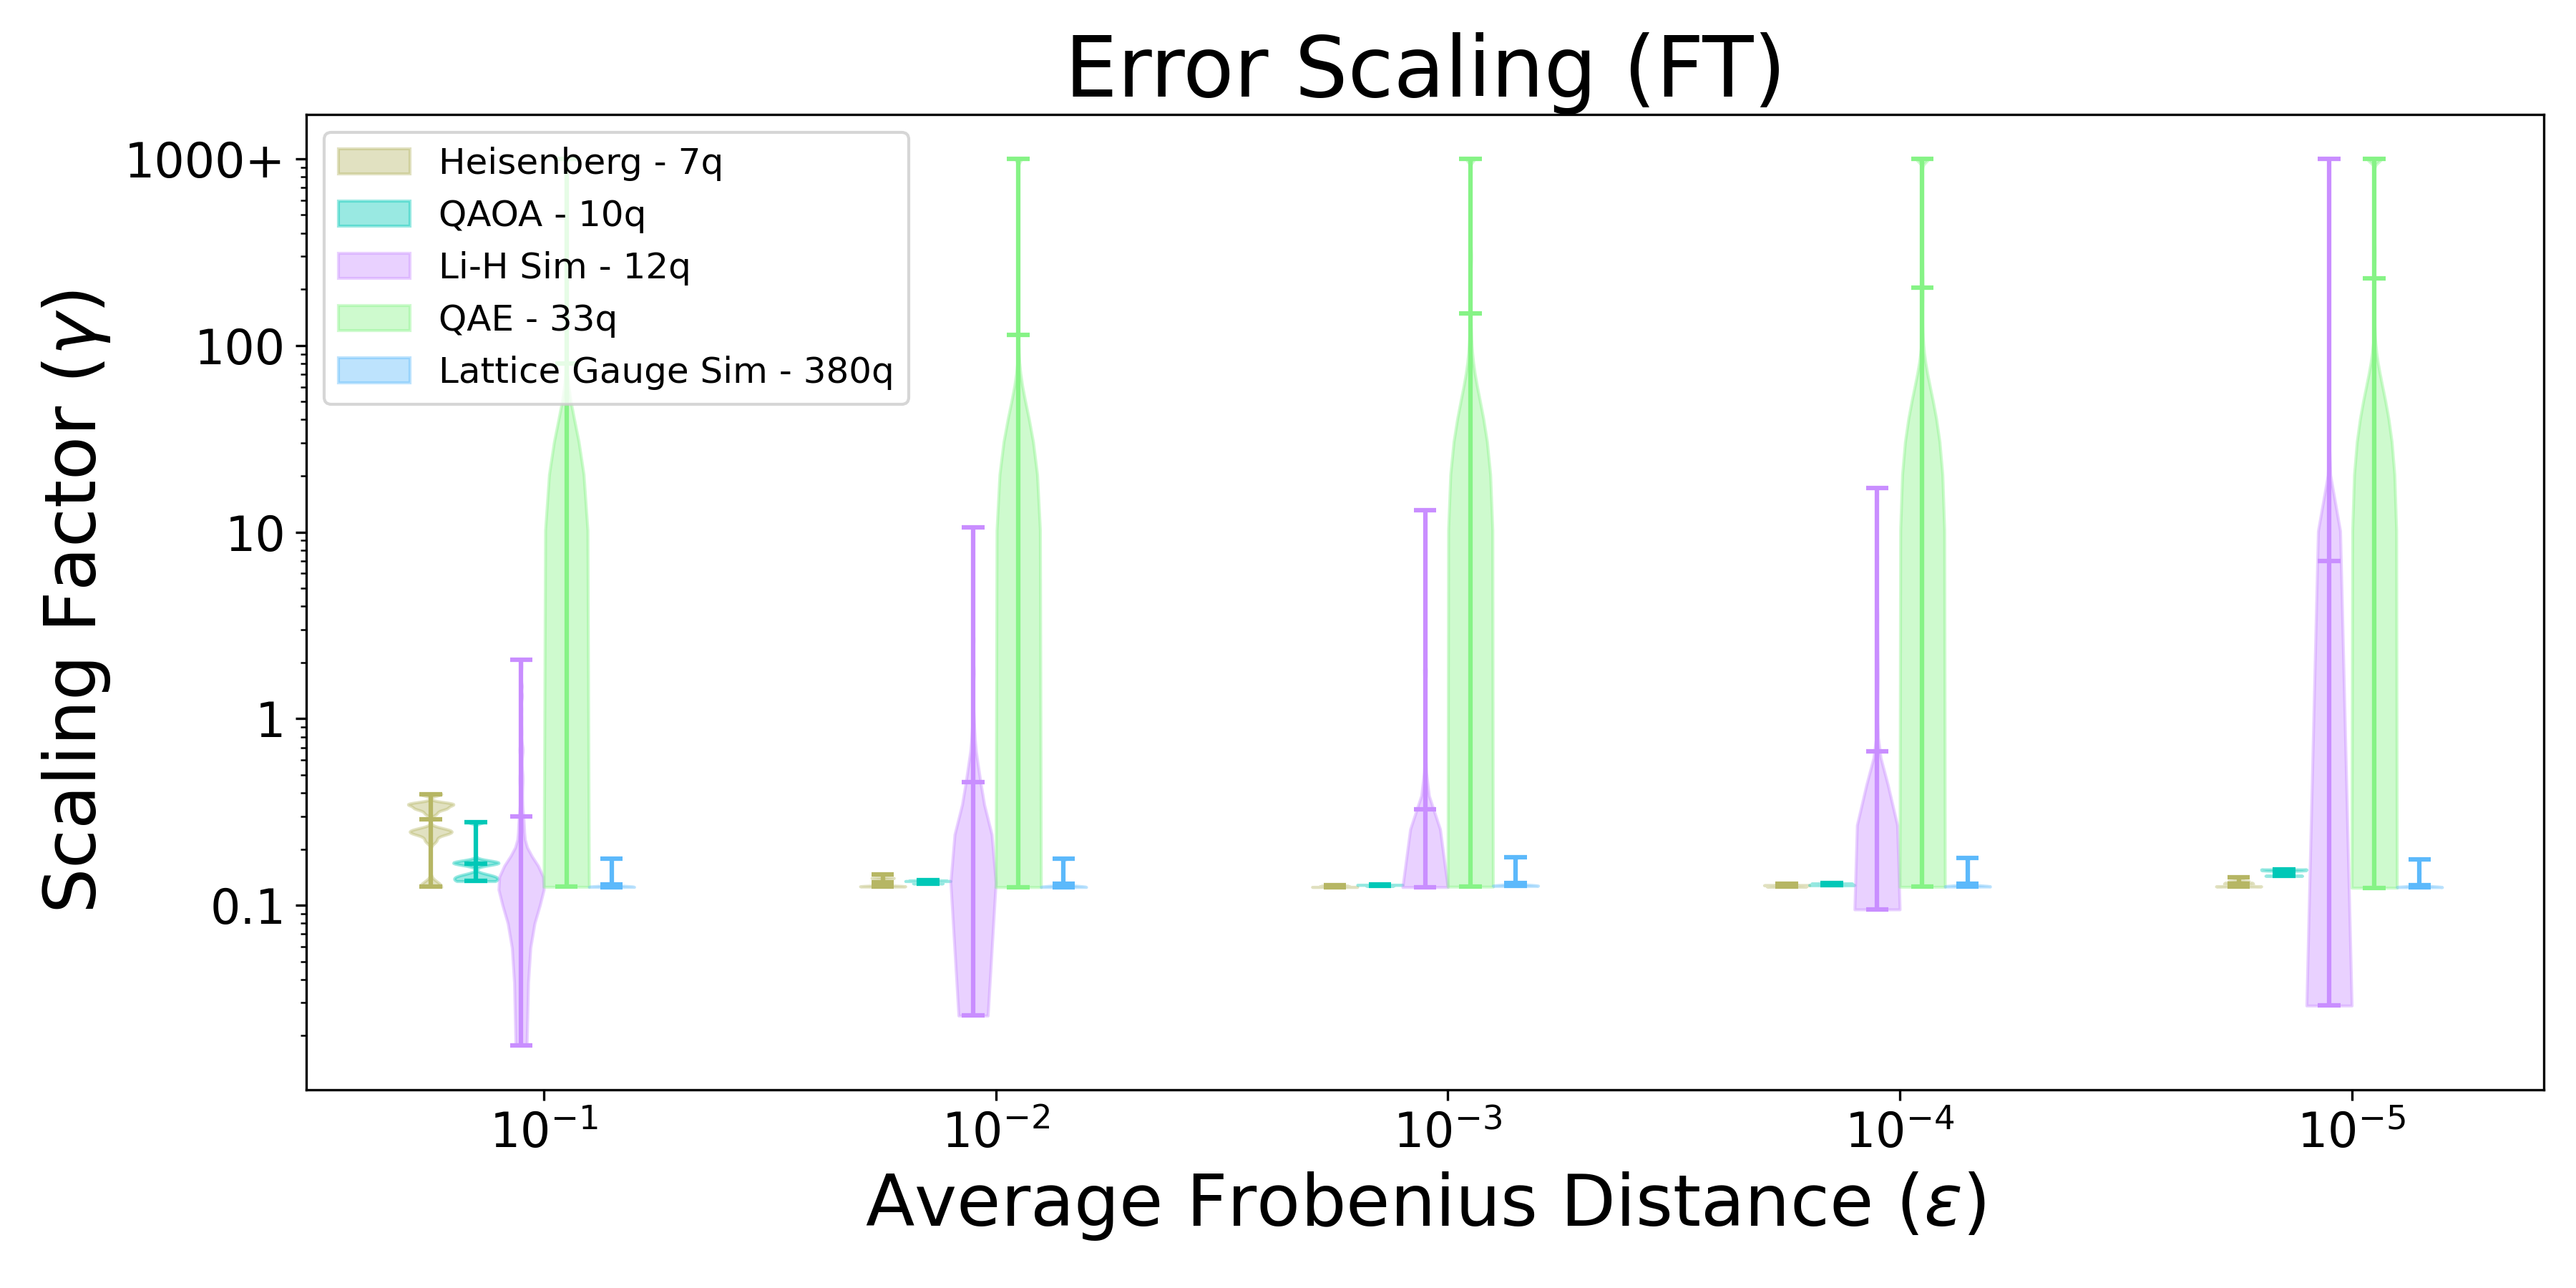
\includegraphics[width=\linewidth]{figures/supplementary/Error_scaling_final_cliff_20.png}
    \end{subfigure}
    \caption{Quadratic scaling factor $\gamma$ as a function of $\epsilon$, for some of the benchmarks.  
    Top: NISQ workflow (minimizing CNOT count).  
    Bottom: FT workflow (minimizing $T$-count).}
    \label{fig:error_scaling}
\end{figure*}


\begin{figure*}[t]
    \centering
    \begin{subfigure}{0.7\textwidth}
        \centering
        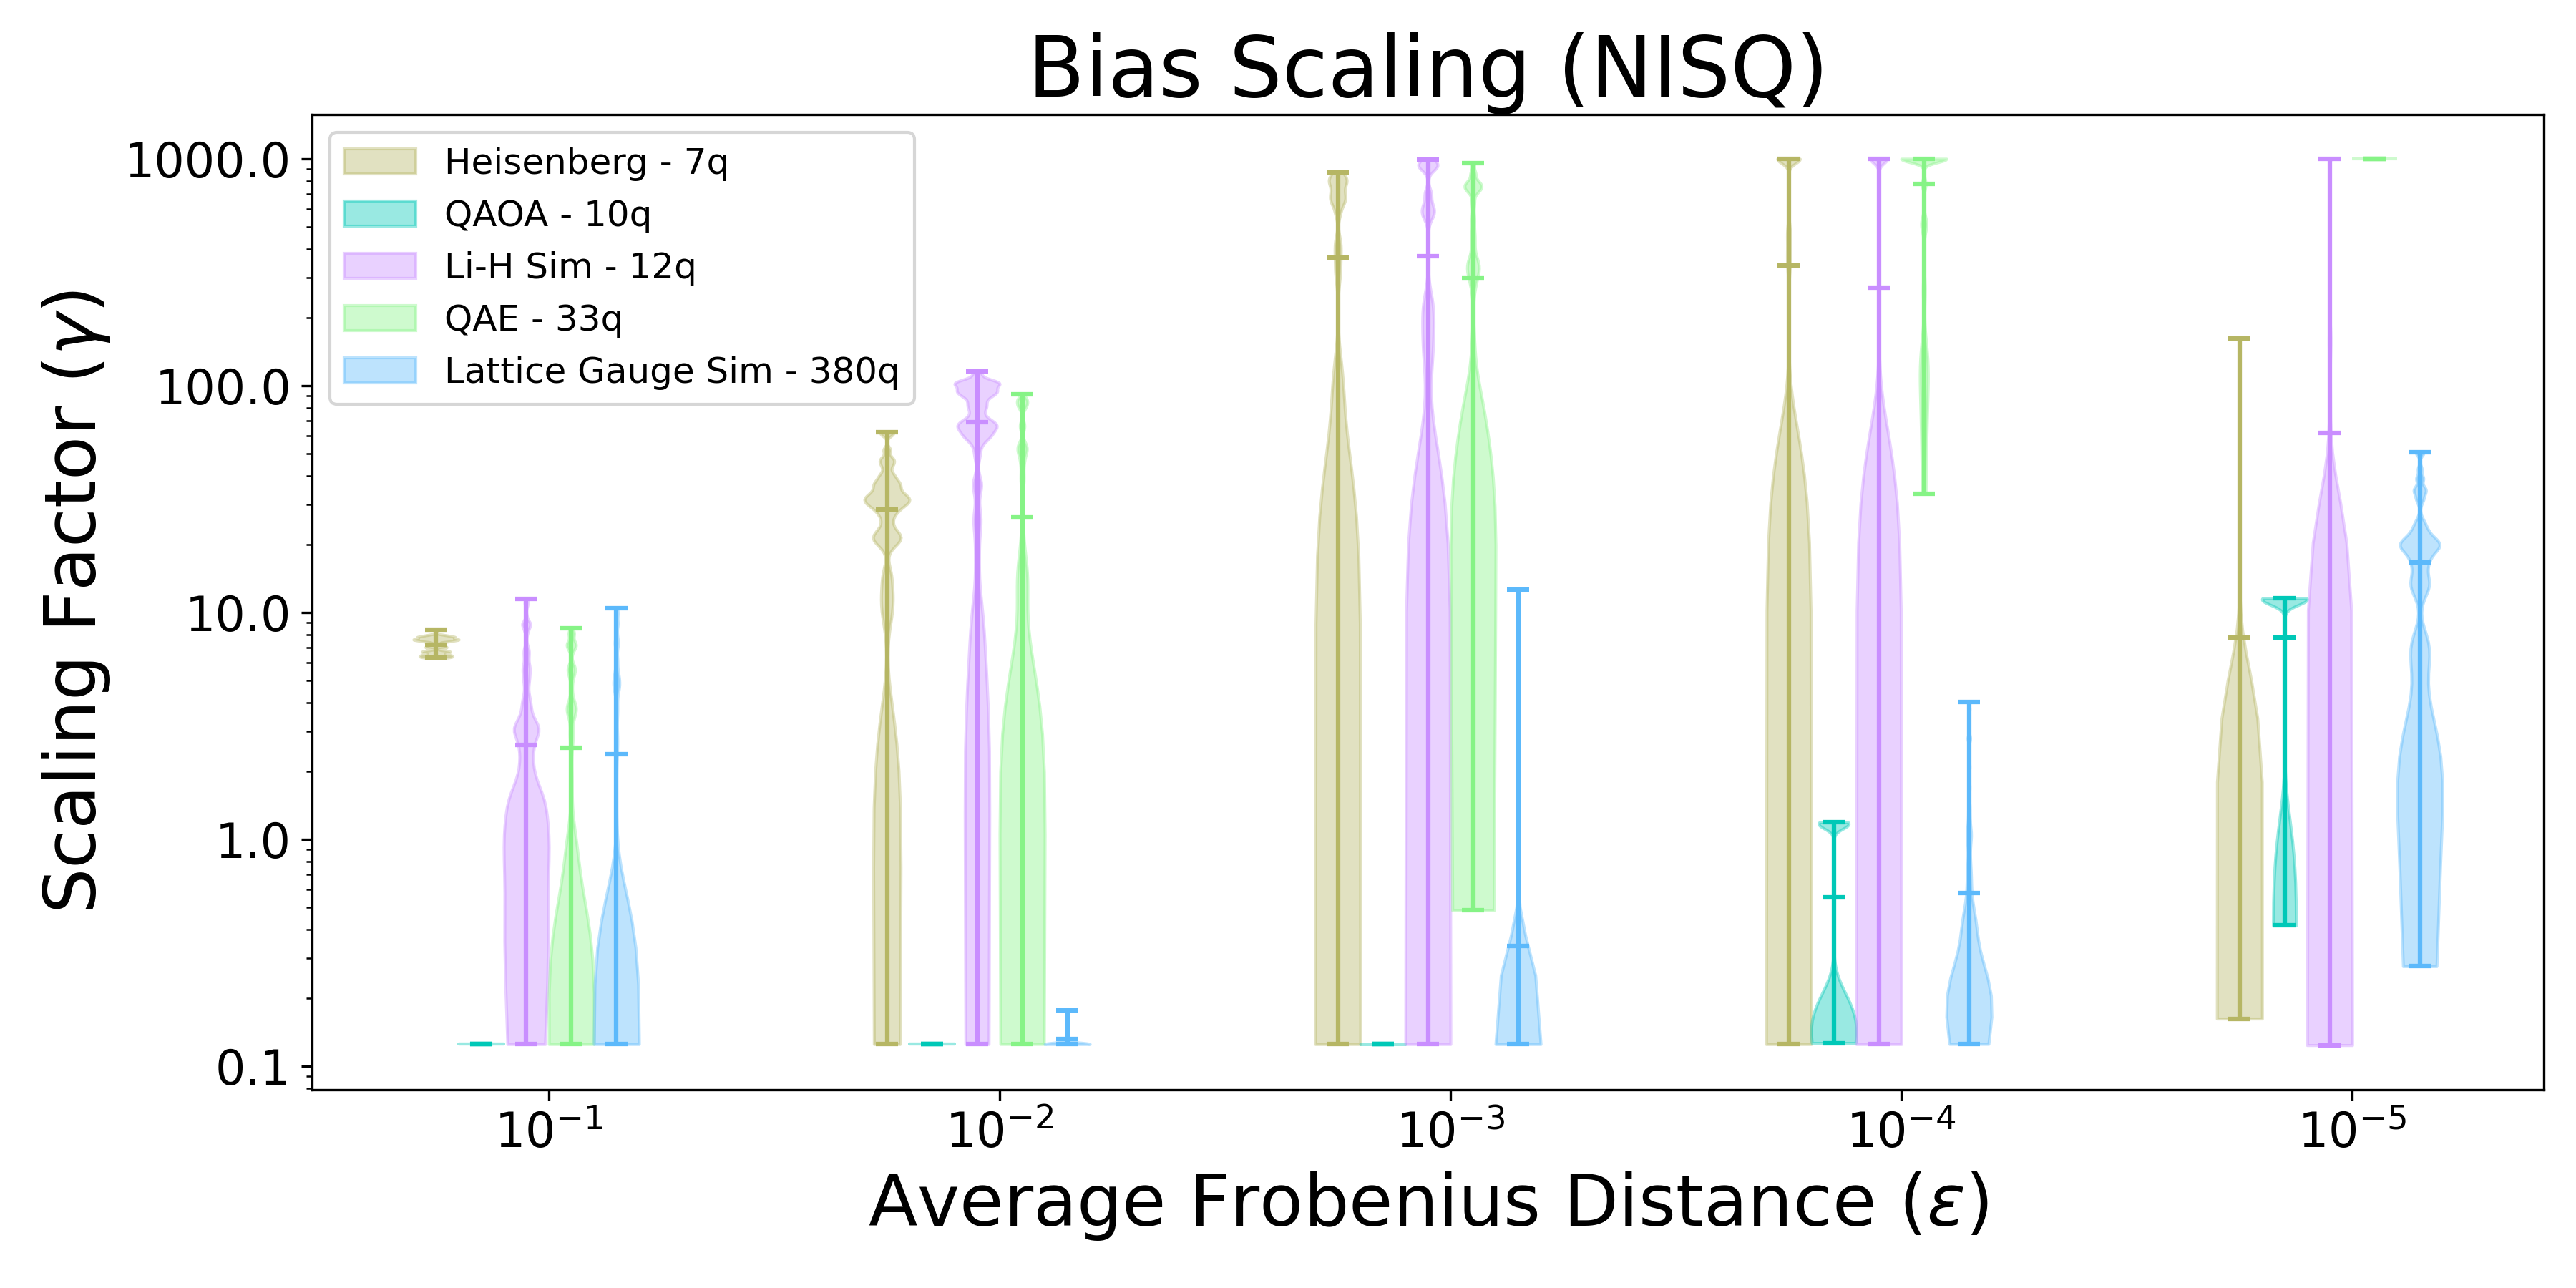
\includegraphics[width=\linewidth]{figures/supplementary/Bias_scaling_final_nisq_20.png}
    \end{subfigure} \\
    \begin{subfigure}{0.7\textwidth}
        \centering
        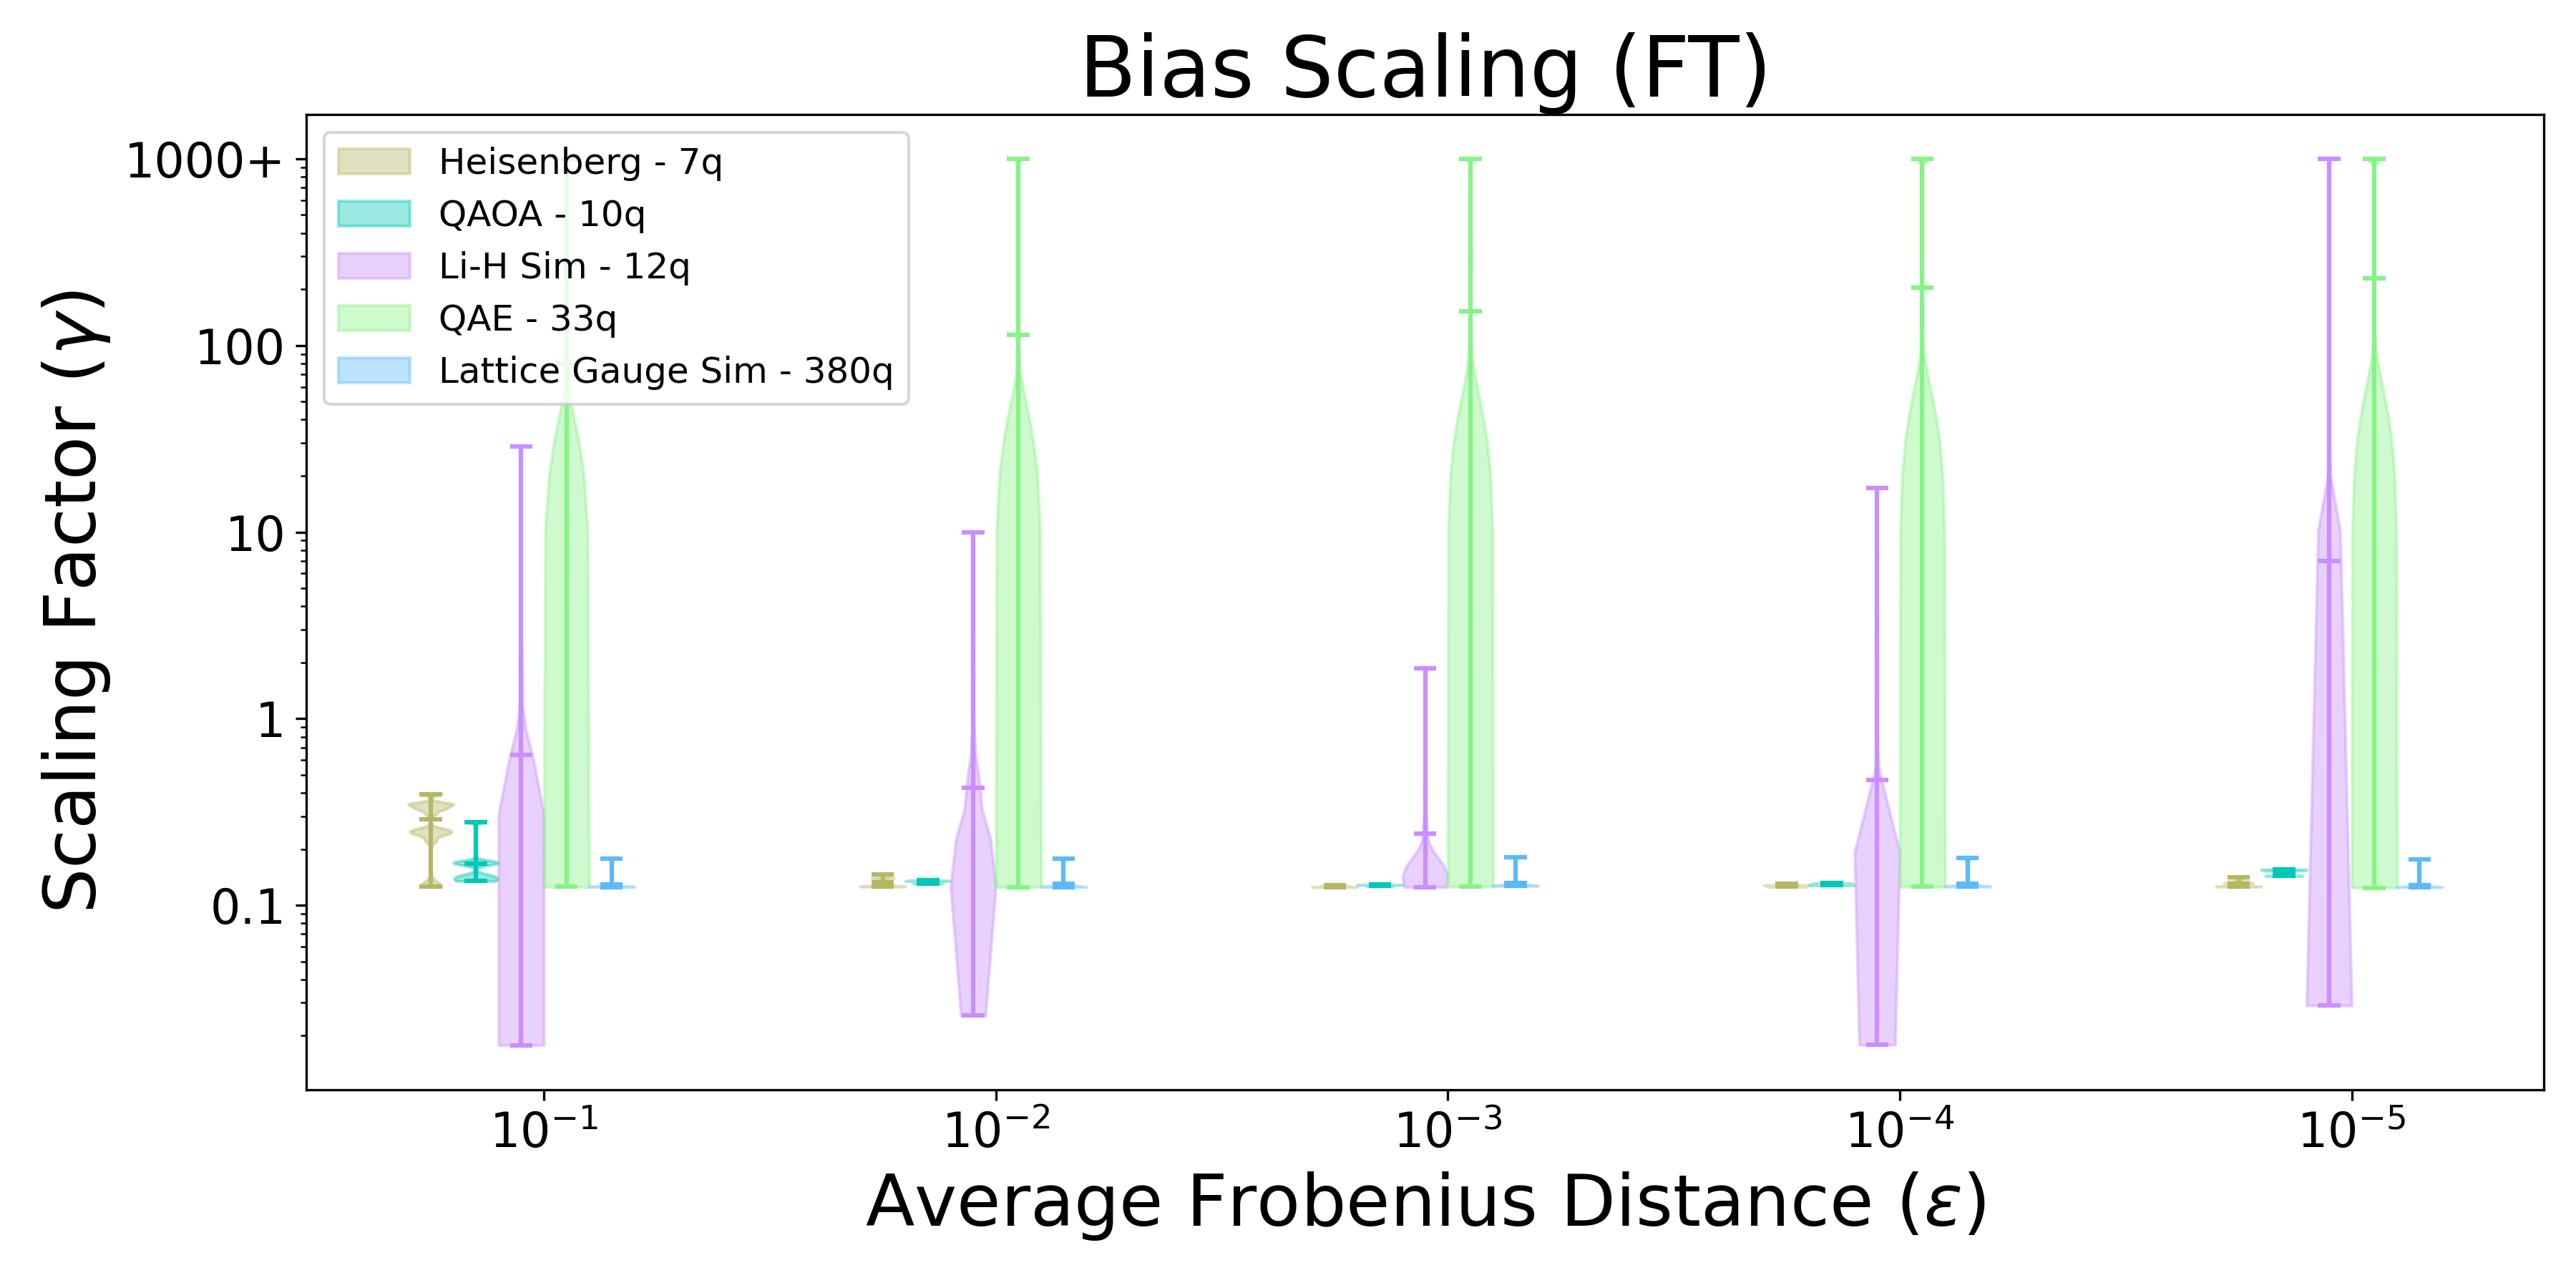
\includegraphics[width=\linewidth]{figures/supplementary/Bias_scaling_final_cliff_20.png}
    \end{subfigure}
    \caption{Quadratic scaling factor for the bias $\gamma_B$ as a function of $\epsilon$, for some of the benchmarks.  
    Top: NISQ workflow (minimizing CNOT count).  
    Bottom: FT workflow (minimizing $T$-count).}
    \label{fig:bias_scaling}
\end{figure*}

Figure \ref{fig:error_scaling} shows violin plots of the \emph{quadratic scaling factor} (QCF),  
\[
\gamma \equiv \frac{\normf{\sum_{i=1}^{M^\k} p^\k_i U^\k_i - V^\k}}{\epsilon^2},
\]  
for all blocks across many of our benchmarks.  
We expect $\gamma = O(1)$ when quadratic reduction of error is achieved.  
The plots indicate that, for most $\epsilon$ values, a significant subset of blocks in both NISQ and FT workflows achieve $O(\epsilon^2)$ scaling. In particular, almost all of the blocks in the FT workflow achieve $O(\epsilon^2)$ scaling. This is because we include a secondary compilation workflow, which trades off numerical synthesis resource reduction for improved scaling.

Our workflow does not require all blocks to satisfy Eq. \eqref{eq:wee_cond}. Blocks that fail to meet the condition are left unmodified, preserving the original circuit for those segments.  
This selective replacement explains why some benchmarks exhibit no gate count reduction (Tables 1 and 2 in the main text, particularly in the NISQ setting at small $\epsilon$). 

We also derived a sufficient condition for satisfying the ReWEE condition in terms of the bias of the compiler output,
\begin{align}
    \normf{\E{U} - V} < O(\epsilon^2).
\end{align}
We can define a quadratic scaling factor for the bias also, $\gamma_B \equiv \normf{\E{U}-V}/\epsilon^2$, and this quantity is displayed in Figure \ref{fig:bias_scaling} for all blocks of many of our benchmarks.


\section{Theoretical proofs}
In this section we provide proofs of Lemma 2 and Lemma 3 in the Methods section of the main text. Before restating the Lemmas and providing proofs, we recall several definitions from the main text.

$V$ is a target unitary on $n$ qubits, and $U_i$ are a set of approximate compilations of $V$ provided by a compiler. The compilation workflow can have probabilistic elements, and therefore we think of $U_i$ as independent, identically distributed (\emph{i.i.d.}) samples from some distribution of approximate compilations. The statistical properties we will demand of the compilation workflow are:
\begin{enumerate}
\item The compilations should all be close to the ideal, in the sense,
    \begin{align}
	\normf{U_i-V} \leq \epsilon, \quad \forall i		
		\label{eq:ass1}
	\end{align}
	\item The compilations have bounded variance, in the sense, $\E{U_i} \equiv \E{U}$ is independent of $i$, and
	\begin{align}
		\E{\normf{U_i - \E{U}}^2} \leq \epsilon', \quad \forall i
		\label{eq:ass2}
	\end{align}
\end{enumerate}
The expectations in these expressions and in the rest of this note are over the distribution of compilations generated by the compiler that satisfy Condition 1, \ie
$ \E{f(U)} = \int {\rm d}\mu_V(U) f(U), $
where ${\rm d}\mu_V(U)$ is the measure over $SU(2^n)$ defined by the compiler output that satisfies Condition 1 when the target is $V$ (the expectation symbol $\E{}$ should have a subscript $V$ but we omit this for ease). In addition,
\begin{enumerate}
    \item Define the channels $\mathcal{V}[\rho] = V \rho V\dg$, $\mathcal{U}_i[\rho] = U_i \rho U_i\dg$, and $\mathcal{U}[\rho] = \sum_i p_i U_i \rho U_i\dg$, for some probabilities $\{p_i\}$.
    \item $J_{\mathcal{E}} \equiv \sum_{i,j=1}^d \mathcal{E}(\ket{i}\bra{j})\otimes \ket{i}\bra{j}$ is the Choi matrix representation of the channel $\mathcal{E}$, which we assume to be acting acting on $d\times d$ density matrices and outputting density matrices of the same size.
\end{enumerate}

\noindent \emph{\bf Lemma 2:} \emph{Let $V$ and $U_i$ be defined as above. Given probabilities $\{p_i\}_{i=1}^M$, ($\sum_{i=1}^M p_i=1$), a sufficient condition for achieving $\E{\normf{\sum_{i=1}^M p_i U_i - V}} \leq O(\epsilon^2)$ is the \emph{reduced bias condition}: $\normf{\E{U}-V} \leq O(\epsilon^2)$.}

\noindent \textit{Proof:} First, note that $\E{\normf{\sum_{i=1}^M p_i U_i - V}} \leq O(\epsilon^2)$ follows directly from $\E{\normf{\sum_{i=1}^M p_i U_i - V}^2} \leq O(\epsilon^4)$ through an application of Jensen's inequality, and so we prove the latter statement.
\begin{align}
    \E{\normf{\sum_{i=1}^M p_i U_i - V}^2} & \leq \E{\normf{\frac{1}{M}\sum_{i=1}^M U_i - V}^2} 
	   = \normf{\overline{bias}}^2 + \frac{1}{M}\overline{var} + \left(1-\frac{1}{M}\right)\overline{covar}, 
       \label{eq:b-v-c} 
\end{align}
where,
\begin{align}
	\overline{bias} &= (\E{U} - V) \label{eq:bias} \\
	\overline{var} &= \frac{1}{M}\sum_{i=1}^{M} \E{\normf{U_i - \E{U}}^2} \label{eq:var} \\
	\overline{covar} &= \frac{1}{M(M-1)}\sum_{i=1}^M \sum_{j \neq i}^M \mathbb{E} \left\{ \tr[(U_i-\E{U})\dg \cdot (U_j - \E{U})] \right\} 
    \label{eq:covar}
\end{align}
The first inequality follows from the fact that the weights $p_i$ are optimized to reduce the ensemble error. The equality on the second line follows from using the definition of the Frobenius norm to decompose the quantity of interest in a \emph{bias-variance-covariance} decomposition, a well-known decomposition of generalization error of ensembles of estimators in machine learning \cite{Ueda_1996, Brown_20005}. Here, $\overline{bias}$ is the bias of the (uniform) ensemble, $\overline{var}$ is the (sample) average of the variance of the members of the ensemble, and $\overline{covar}$ is the covariance of the ensemble members. Since the ensemble members are sampled \emph{i.i.d.} from the compiler output distribution, the covariance term is zero. In addition, using the fact that the samples have bounded variance, Eq. \eqref{eq:ass2}, we get
$\E{\normf{\sum_{i=1}^M p_i U_i - V}^2} \leq \normf{\E{U}-V}^2 + \frac{\epsilon'}{M}$.
This quantity can be bounded as $O(\epsilon^4)$ by satisfying the reduced bias condition and choosing $M \geq \epsilon'/\epsilon^4$. \QED
\\

\noindent \emph{\bf Lemma 3:} \emph{Let $V$ and $U_i$ be defined as above, and let these unitaries act on a register of $n$ qubits; \ie ${\rm dim}~ V = {\rm dim}~ U_i = 2^n \equiv d$. Define $\mathcal{V}[\rho] = V \rho V^{\dagger}$ as a target channel, and $\mathcal{U}[\rho] = \sum_{i=1}^M p_i U_i \rho U_i\dg$ as an optimized ensemble channel, such that $d_\diamond(\mathcal{V}, \mathcal{U})\leq O(\epsilon^2)$. Further, let $\hat{\mathcal{U}}[\rho] = \frac{1}{T}\sum_{i=1}^T U_{\sigma(i)} \rho U_{\sigma(i)}\dg$ be the empirical channel defined by sampling and averaging over $U_i$ according to the distribution $\{p_i\}$ -- \ie $\sigma(i) \in \{1,...,M\}$. For $\epsilon, \delta \in (0,1)$, $\pr\left\{ d_\diamond(\mathcal{V}, \hat{\mathcal{U}}_T) \leq O(\epsilon^2) \right\} > 1-\delta$, given
\begin{align}
    T \geq \frac{2v + \frac{2}{3}R \left(\epsilon^2/(2d^2)\right) }{\left(\epsilon^2/(2d^2)\right)^2}\log \frac{2d^2}{\delta}
    \label{eq:T_bound}
\end{align}
Here, $v \equiv \normo{\sum_{i=1}^M p_i (J_i - J_{\mathcal{U}})^2}, R \equiv \max_i \normo{J_i - J_{\mathcal{U}}}$, and $J_i (and J_{\mathcal{U}}$) are the $d^2$-dimensional Choi matrices associated to the channel $\mathcal{U}_i[\rho] = U_i \rho U_i^{\dagger}$ (and $\mathcal{U}$).}

\noindent \textit{Proof:} We begin by an application of the triangle inequality:
\begin{align}
    d_\diamond(\mathcal{V}, \hat{\mathcal{U}}) &\leq  d_\diamond(\mathcal{V}, \mathcal{U}) +  d_\diamond(\mathcal{U}, \hat{\mathcal{U}}) \nn \\  
    & = O(\epsilon^2) + d_\diamond(\mathcal{U}, \hat{\mathcal{U}}),
    \label{eq:lemma3_1}
\end{align}
and hence we are left with the task of determining the sample size $T$ necessary to satisfy $d_\diamond(\mathcal{U}, \hat{\mathcal{U}}) \leq \epsilon^2$. Therefore, 
\begin{align}
    d_\diamond(\mathcal{U}, \hat{\mathcal{U}}) &\equiv \normd{\mathcal{U}- \hat{\mathcal{U}}} \nn \\
    & \leq \normt{J_\mathcal{U} - J_{\hat{\mathcal{U}}}} \nn \\
    & \leq 2d^2 \normo{J_\mathcal{U} - J_{\hat{\mathcal{U}}}},
\end{align}
where the first inequality follows from an identity established by Watrous \cite[Exercise 3.6]{watrous_2018}, the second is the application of a standard norm inequality ($\normt{A}\leq {\rm rank}(A)\normo{A}$), and an overestimate of the relevant rank: ${\rm rank}(J_\mathcal{U} - J_{\hat{\mathcal{U}}}) \leq {\rm rank}(J_\mathcal{U} ) + {\rm rank}(J_{\hat{\mathcal{U}}}) \leq 2d^2$. In the above, the Choi matrices are explicitly, $J_\mathcal{U} = \sum_{i=1}^M p_i J_i$ and $J_{\hat{\mathcal{U}}} = \frac{1}{T} \sum_{i=1}^T J_i$, with $J_i \equiv J_{\mathcal{U}_i}$. 

Now that the error is expressed in terms of an operator norm, we can apply standard Bernstein matrix concentration inequality \cite{tropp_2015} to get, 
\begin{align}
    \pr\left\{ d_\diamond(\mathcal{U}, \hat{\mathcal{U}}) \geq \epsilon^2 \right\} \leq \pr\left\{ \normo{J_\mathcal{U} - J_{\hat{\mathcal{U}}}} \geq \frac{\epsilon^2}{2d^2} \right\} \leq 2d^2 \exp\left(-\frac{T(\frac{\epsilon^2}{2d^2})^2}{2v + \frac{2}{3}R \frac{\epsilon^2}{2d^2}}\right),
\end{align} 
where $v$ and $R$ are the variance and maximum deviation as defined in the Lemma statement. In order for the right-hand side to be at most $\delta$, the sample size given in Eq. \eqref{eq:T_bound} is sufficient. Finally, combining this with the statement in Eq. \eqref{eq:lemma3_1} yields the Lemma statement. 
\QED

\subsection{Statistics of factors entering sample complexity}
While the formal sample complexity bound in Lemma 3 scales with $\epsilon$ as $O(1/\epsilon^4)$, in the main text we claimed that in practice, $v=O(\epsilon^2)$, and therefore, the number of samples needed is $O(1/\epsilon^2)$. Figure 5 in the main text provided evidence for this gentler scaling for one of the benchmarks in our study. While Lemma 3 is stated in terms of diamond distance between the empirical channel and the ensemble channel, this error is infeasible to evaluate numerically because of the difficulty of calculating the diamond distance for channels acting on many qubits. Therefore, in Figure 5 of the main text, we showed the trace distance error in the output, $\normt{\rho_{T} - \rho_i}$,
where $\rho = \sum_{i=1}^M p_i U_i \rho_{0} U_i\dg$ is the output of the ensemble channel for random input state $\rho_{0}$, and $\rho_{T} = \frac{1}{T}\sum_{i=1}^T U_i \rho_{0} U_i\dg$ is the output of the empirical channel for the same input (the $U_i$ in the empirical channel are sampled according to the distribution $\{p_i\}$ set by the ensemble channel). 

The equivalent sample complexity bound for this error metric is $\pr\{\normt{\rho_{T} - \rho} \geq \epsilon^2\} \leq 1-\delta$, if
\begin{align}
    T \geq \frac{2v + \frac{2}{3}R \left(\epsilon^2/(2d)\right) }{\left(\epsilon^2/(2d)\right)^2}\log \frac{2d}{\delta},
    \label{eq:T_bound_state} 
\end{align}
where $v \equiv \normo{\sum_{i=1}^M p_i (\rho_i - \rho)^2}, R \equiv \max_i \normo{\rho_i - \rho}$, and $\rho_i = U_i\rho_0 U_i\dg$. Calculating the values $v$ and $R$ is difficult for most of the benchmarks we studied, even in this case, because $M$ can be very large for full circuits, and thus computing the ideal ensemble output $\rho$ is numerically intensive. Instead, we compute these variance and maximum deviation values, $v$ and $R$, for all blocks in two of our benchmark circuit ensembles. As shown in Fig. \ref{fig:vR}, $v \ll \epsilon^2$ in practice, which explains the gentler scaling of $T$ required to approximate the ensemble channel with the empirical channel.

\begin{figure*}[ht]
    \centering
        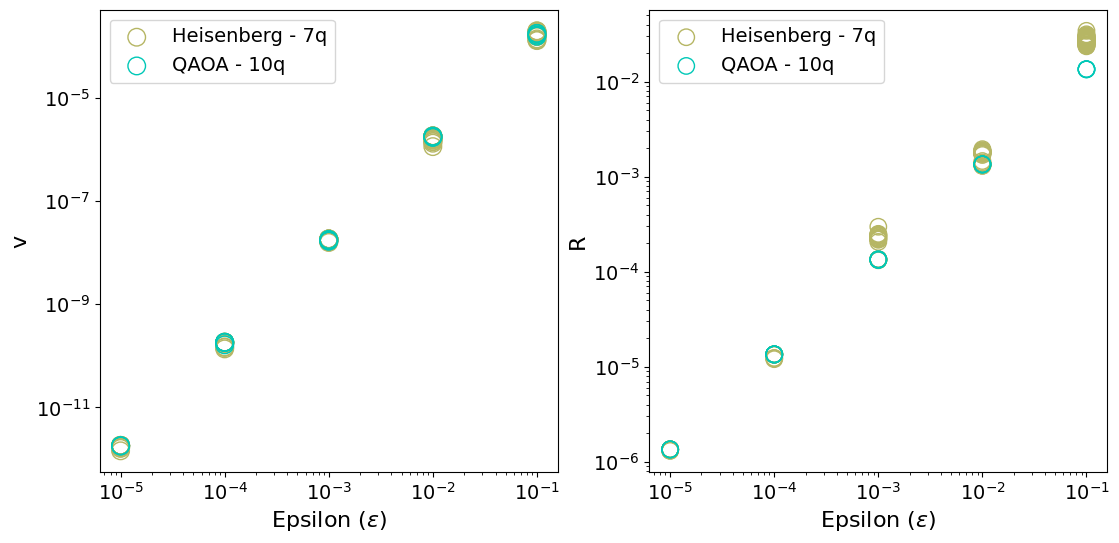
\includegraphics[width=0.7\linewidth]{figures/supplementary/v_R_all_circs_1_final.png}
    \caption{Values of variance and maximum deviation factors, $v$ and $R$, entering the sample complexity bound Eq. \eqref{eq:T_bound_state} for each block of two benchmark circuits.}
    \label{fig:vR}
\end{figure*}

\newpage

\input{si.bbl}

\end{document}


\end{document}


\end{document}


\end{document}
